%%%%%%%%%%%%%%%%%%%%%%%%%%%%%%%%%%%%%%%%%%%%%%%%%%%%%%%%%%%%%%%%%%%%%%
% Lớp 11 | Hàm số mũ và hàm số lôgarít | Hàm số mũ. Hàm số lôgarít
% Dạng 1D6?3-3: Sự biến thiên và đồ thị của hàm số mũ, lôgarít
% Số câu: 141  (sinh tự động bởi tach_cau.py; từ nay thầy sửa trực tiếp file này)
%%%%%%%%%%%%%%%%%%%%%%%%%%%%%%%%%%%%%%%%%%%%%%%%%%%%%%%%%%%%%%%%%%%%%%

%%%%%%%%%%%%%%%% TRẮC NGHIỆM 4 PHƯƠNG ÁN %%%%%%%%%%%%%%%%

% nguồn: Ok_TracNghiemLop11_Lan1
\begin{ex}%[1D6N3-3]%[ma:a5b4bcaf]
	Hàm  số nào dưới đây đồng biến trên khoảng $(0;+\infty)$?
	\choice 
		{\True  $y=\log_{\sqrt{3}}x$}
		{$y=\log_{\frac{\pi}{6}}x$} 
		{$y=\log_{\frac{e}{3}}x$} 
		{$y=\log_{\frac{1}{4}}x$} 
	\loigiai{ 
		Hàm số $y=\log_ax$ đồng biến trên khoảng $(0;+\infty)$ khi và chỉ  khi $a>1$.\\
		Vậy hàm  số $y=\log_{\sqrt{3}}x$ đồng biến trên $(0;+\infty)$.
	 }
\end{ex}

% nguồn: Ok_TracNghiemLop11_Lan1
\begin{ex}%[1D6N3-3]%[ma:df23a661]
	Trong các hàm số sau hàm số  nào nghịch biến trên $\mathbb{R}$?
	 \choice
		 {$\log_3x^2$}
		{$y=\log(x^3)$} 
		{\True $y=\left(\dfrac{\mathrm{e}}{4}\right)^x$} 
		 {$y=\left(\dfrac{2}{5}\right)^{-x}$}
	 \loigiai{
		Hàm số  $y=a^x$ nghịch biến trên $\mathbb{R}\Leftrightarrow 0<a<1$.\\
		Vì $0<\dfrac{\mathrm{e}}{4}<1$ nên hàm số $y=\left(\dfrac{\mathrm{e}}{4}\right)^x$ nghịch biến  trên $\mathbb{R}$.
	 }
\end{ex}

% nguồn: Ok_TracNghiemLop11_Lan1
\begin{ex}%[1D6N3-3]%[ma:b43582df]
	\immini{Cho hàm  số $y=\log_a x\ \left(0<a\neq 1\right)$ có đồ thị như hình vẽ. Khẳng định nào sau đây là đúng?
	 \choice
		{Hàm  số nghịch biến trên $\mathbb{R}$}
		{Hàm số  nghịch biến trên $\left(0;+\infty\right)$}
		{Hàm số đồng biến  trên $\mathbb{R}$}
		{\True Hàm  số đồng biến trên $\left(0;+\infty\right)$}
	\loigiai{Hàm số đồng biến trên  $\left(0;+\infty\right)$}}
	{\begin{tikzpicture}[scale=1,line join=round,>=stealth,font=\footnotesize]
		\draw[->]  (-1,0) -- (4,0) node[below] {$x$};
		\draw[->]  (0,-1) -- (0,3) node[left] {$y$};
		\draw (0,0)  node[below left]{$O$};
		\draw[samples=150,smooth,domain=0.5:3.5] plot  (\x,{log2 (\x)});
	\end{tikzpicture}
	} 
\end{ex}

% nguồn: Ok_TracNghiemLop11_Lan1
\begin{ex}%[1D6N3-3]%[ma:21c63876]
	\immini{ 
	Đường cong  trong hình vẽ bên là đồ thị của hàm số nào dưới đây?
	\choice 
		 {$y=-\mathrm{e}^x$}
		{$y=\left|\ln x\right|$} 
		 {\True $y=\ln x$}
		 {$y=\mathrm{e}^x$}
		} 
		{\begin{tikzpicture}[scale=1,line join=round,line cap=round,>=stealth,font=\footnotesize]
		\draw[->] (-0.5,0)--(0,0) node[below  left]{$O$}--(4,0) node[below]{$x$};
		\draw[->] (0,-1.5)  --(0,2) node[right]{$y$};
		\begin{scope}
			\clip (-0.5,-1.5) rectangle (4,2); 
			 \draw[domain=0.25:4,samples=100]plot (\x,{ln(\x)});
		\end{scope}
		\draw[dashed] (2.7,0) node[below]{$\mathrm{e}$}  -- (2.7,1) -- (0,1) node[left]{$1$};
		\draw  (1,0) node[below]{$1$};
		\draw[fill] (0,0)  circle (1pt)
			(0,1) circle  (1pt)
			(1,0)  circle (1pt)
			 (2.7,0) circle (1pt)
			(2.7,1) circle (1pt); 
	\end{tikzpicture}
		} 
	 \loigiai{
		Đồ thị hàm số đi qua điểm $(\mathrm{e};1)$ và nằm cả trên và dưới trục hoành nên chỉ có hàm số $y=\ln  x$ thoả mãn.
	 }
\end{ex}

% nguồn: Ok_TracNghiemLop11_Lan1
\begin{ex}%[1D6N3-3]%[ma:fd6665b0]
	Hàm số nào sau đây đồng biến trên tập  xác định của nó?
	 \choice
		 {$y=\log _{\frac{1}{3}} x$}
		{$y=\left(\dfrac{1}{2}\right)^x$} 
		{$y=\left(\dfrac{\pi}{5}\right)^x$} 
		{\True $y=\log  _{\sqrt{2}} x$}
	\loigiai{ 
		 Vì $\sqrt{2}>1$ nên hàm số $y=\log _{\sqrt{2}} x$ đồng biến trên $(0;+\infty)$.
	 }
\end{ex}

% nguồn: Ok_TracNghiemLop11_Lan1
\begin{ex}%[1D6N3-3]%[ma:ef82fc0b]
	Hàm số nào  sau đây nghịch biến trên tập xác định của nó?
	 \choice
		{$y=\log_\pi x$} 
		 {$y=\log_3x$}
		{$y=\log_{\sqrt{3}}x$} 
		 {\True $y=\log_{\frac{1}{\mathrm{e}}}x$}
	 \loigiai{
		Hàm số  $y=\log_{\frac{1}{e}}x$ nghịch biến trên tập xác định của nó vì $0<\dfrac{1}{\mathrm{e}}<1$.
	} 
\end{ex}

% nguồn: Ok_TracNghiemLop11_Lan1
\begin{ex}%[1D6N3-3]%[ma:a5b1c189]
	Hàm số $y=\log_2x$ có đồ thị đi qua điểm  nào sau đây?
	 \choice
		 {$(0;1)$}
		 {$(1;1)$}
		 {$(2;2)$}
		{\True $(2;1)$} 
	\loigiai{ 
		Ta có $\log_22=1$ nên  đồ thị hàm số $y=\log_2x$ đi qua điểm $(2;1)$.
	 }
\end{ex}

% nguồn: Ok_TracNghiemLop11_Lan1
\begin{ex}%[1D6N3-3]%[ma:ac2777f8]
	 \immini{
	Đường cong trong hình bên là đồ thị của hàm  số nào?
	\choice 
		{\True $y=2^x$} 
		{$y=\log_2 x$} 
		 {$y=x^2$}
		{$y=\left(\dfrac{1}{2}\right)^x$} 
		}{ 
		\begin{tikzpicture}[>=stealth]
				\draw[->] (-2.5,0) -- (2.5,0) node[below] {$x$}; 
				\draw[->] (0,-1) -- (0,3)  node[left] {$y$};
				\draw[fill] (0,0) node[below  right]{$O$} circle (1pt);
				\draw (0,1) node[above left]{$1$}; 
				\begin{scope}
					\clip (-2,-0.5) rectangle  (2,3);
					\draw[smooth,samples=200,domain=-2:2.01] plot  (\x,{(2)^(\x)});
				\end{scope}
			\end{tikzpicture}
		} 
	 \loigiai{
		Dựa vào đồ thị ta thấy, đồ thị trên là đồ thị của hàm số mũ có cơ số $a>1$. Trong các phương án chỉ có hàm số $y = 2^x$  thỏa mãn.
	 }
\end{ex}

% nguồn: Ok_TracNghiemLop11_Lan1
\begin{ex}%[1D6N3-3]%[ma:7c220a15]
	\immini{Đường cong  trong hình bên là đồ thị của một hàm số trong bốn hàm số được liệt kê ở bốn phương án $A$, $B$, $C$, $D$ dưới đây. Hỏi hàm số đó là hàm số nào?
	\choice 
		{\True  $y=\log_2x$}
		{$y=\log_{\sqrt{2}}x$} 
		 {$y=\log_2{2x}$}
		{$y=\log_{\tfrac{1}{2}}x$}}{	\begin{tikzpicture}[scale=.5,font=\footnotesize,
			line join=round,line  cap=round,>=stealth]
		\draw[->,line  width = 1pt] (-2,0)--(0,0) node[below left]{$O$}--(4,0) node[below]{$x$};
		 \draw[->] (0,-3.5) --(0,3) node[right]{$y$};
		\draw (0.5,0) node[above]{$\dfrac{1}{2}$} circle  (1pt);
		\draw (1,0) node[below]{$1$}  circle (1pt);
		\draw [smooth,samples=290,domain=0.1:4] plot (\x,{ln(\x)/ln(2)}); 
		 \draw [dashed] (0.5,0)--(0.5,-1)--(0,-1) node[left]{$-1$} circle (1pt);
	\end{tikzpicture}
		} 
	 \loigiai{
		Ta thấy đồ thị hàm số đi qua điểm $A\left(\dfrac{1}{2};-1\right)$ nên  thỏa mãn $y=\log_2x$.
	 }
\end{ex}

% nguồn: Ok_TracNghiemLop11_Lan1
\begin{ex}%[1D6N3-3]%[ma:ee02f1bb]
	Cho hàm số $y=\log_{\sqrt{5}}x$. Mệnh đề  nào dưới đây là mệnh đề \textbf{sai}?
	 \choice
		{Hàm số  đã cho đồng biến trên tập xác định}
		{\True Hàm số đã cho  có tập xác định $\mathscr{D}=\mathbb{R} \setminus \{0\}$}
		{Đồ  thị hàm số đã cho có một tiệm cận đứng là trục tung}
		{Đồ thị hàm số đã cho không có tiệm  cận ngang}
	 \loigiai{
		Ta có tập xác định của hàm  số $y=\log_{\sqrt{5}}x$ là $\mathscr{D}=(0;+\infty)$. \\
		Do đó mệnh đề \lq\lq Hàm  số đã cho có tập xác định $\mathscr{D}=\mathbb{R} \setminus \{0\}$\rq\rq là mệnh đề sai.
	 }
\end{ex}

% nguồn: Ok_TracNghiemLop11_Lan1
\begin{ex}%[1D6N3-3]%[ma:bb431404]
	 Chọn khẳng định sai trong các khẳng định sau:
	 \choice
		{\True Hàm số $y=\log_2 x$ đồng biến trên $\mathbb{R}$} 
		{Hàm số $y=\log _{\tfrac{1}{2}} x$ nghịch biến trên tập xác định của  nó}
		{Hàm số $y=2^x$  đồng biến trên $\mathbb{R}$}
		{Hàm số $y=x^{\sqrt{2}}$ có tập xác định  là $\left(0;+\infty \right)$}
	 \loigiai{
		 Hàm số $y=\log_2 x$ đồng biến trên khoảng $\left(0;+\infty \right)$.
	} 
\end{ex}

% nguồn: Ok_TracNghiemLop11_Lan1
\begin{ex}%[1D6N3-3]%[ma:98d0ad83]
	Hàm số nào dưới đây nghịch  biến trên tập xác định của nó?
	 \choice
		{$y=\log_{\sqrt{3}}x$} 
		 {$y=\log_2\left(\sqrt{x}+1\right)$}
		{\True $y=\log_{\frac{\pi}{4}}x$} 
		 {$y=\left(\dfrac{\pi}{3}\right)^x$}
	 \loigiai{
		Hàm số $y=\log_{\frac{\pi}{4}}x$ có  tập xác định $\mathscr{D}=(0;+\infty)$.\\
		Nhận thấy cơ  số $\dfrac{\pi}{4}<1$ nên $y=\log_{\frac{\pi}{4}}x$ nghịch biến trên tập xác định.
	 }
\end{ex}

% nguồn: Ok_TracNghiemLop11_Lan1
\begin{ex}%[1D6N3-3]%[ma:7dc78bc5]
	 Trong bốn hàm số sau, hàm số nào nghịch biến trên $\mathbb{R}$?
	 \choice
		 {$y=2024^x$}
		{$y=\left(\dfrac{2024}{2023}\right)^x$} 
		 {$y=\log_{2024}x$}
		{\True $y=\left(\dfrac{2023}{2024}\right)^x$} 
	 \loigiai{
	Hàm số $y=\left(\dfrac{2023}{2024}\right)^x$ nghịch biến trên $\mathbb{R}$ do cơ số $\dfrac{2023}{2024}\in(0; 1)$.} 
\end{ex}

% nguồn: Ok_TracNghiemLop11_Lan1
\begin{ex}%[1D6N3-3]%[ma:fd2e4ef6]
	Trong các khẳng định sau,  khẳng định nào \textbf{sai}?
	 \choice
		{\True Hàm số $y = \log_{2}x$ đồng biến trên $\mathbb{R}$} 
		{Hàm số $y = \log_{\frac{1}{2}}x$ nghịch biến  trên tập xác định của nó}
		{Hàm số  $y = 2^x$ đồng biến trên $\mathbb{R}$}
		{Hàm số $y = x^{\sqrt{2}}$ có tập xác định là $\left(0;  +\infty\right)$}
	 \loigiai{
		Do hàm số lô-ga-rít có tập xác định $\mathscr{D} = \left(0; +\infty\right)$ nên khẳng  định sai là: Hàm số $y = \log_{2}x$ đồng biến trên $\mathbb{R}$.
	} 
\end{ex}

% nguồn: Ok_TracNghiemLop11_Lan1
\begin{ex}%[1D6N3-3]%[ma:56e78d6c]
	Trong các hàm số sau hàm số nào nghịch biến trên $\mathbb{R}$? 
	 \choice
		 {${\log }_{3}{x^2}$}
		{$y=\log \left(x^3\right)$} 
		{\True $y=\left( \dfrac{\mathrm{e}}{4}  \right)^x$}
		 {$y=\left( \dfrac2{5} \right)^{-x}$}
	\loigiai{ 
		Hàm số mũ $y=a^x$ với $0<a<1$ nghịch biến trên $\mathbb{R}$.\\ 
		Ta có $0<\dfrac{\mathrm{e}}{4}<1$ nên hàm số $y={{\left( \dfrac{\mathrm{e}}{4} \right)}^x}$  nghịch biến trên $\mathbb{R}$.
	} 
\end{ex}

% nguồn: Ok_TracNghiemLop11_Lan1
\begin{ex}%[1D6N3-3]%[ma:ef371a61]
	\immini 
	 {
	 Hàm số nào có đồ thị như đường cong trong hình vẽ bên?
	 \choice
		 {$y=\left(\dfrac{1}{2}\right)^x$}
		{$y=\log_2x$} 
		{\True  $y=2^x$}
		 {$y=\log_{\tfrac{1}{2}}x$}
		 }
		{ 
		\begin{tikzpicture}[>=stealth,line join=round,line cap=round,font=\footnotesize,scale=1]
				\draw[->] (-3,0)--(3,0) node[below]  {$x$};
				\draw[->] (0,-1.5)--(0,3) node[left] {$y$}; 
				\clip  (-3,-1.5) rectangle (3,3);
				\draw[smooth,samples=100,domain=-3:3] plot (\x,{2^(\x)}); 
				\draw[fill] 
					(0,0) circle  (1pt) node[below left] {$O$}
					(1,0) circle (1pt)  node[below] {$1$}
					(0,1)  circle (1pt) node[left] {$1$}
					(0,2) circle (1pt) node[left]  {$2$};
				 \draw[dashed] (1,0)|-(0,2);
			\end{tikzpicture}
		} 
	\loigiai{ 
	Vì đồ thị hàm số luôn nằm trên trục hoành nên đây là  đồ thị của hàm số mũ.\\
	Vì hàm số đồng biến trên $\mathbb{R}$ nên cơ số  phải lớn hơn $1$.\\
	Do đó hàm số cần tìm  là $y=2^x$.
	 }
\end{ex}

% nguồn: Ok_TracNghiemLop11_Lan1
\begin{ex}%[1D6N3-3]%[ma:429d0ec6]
	Trong  các hàm số sau đây, hàm số nào nghịch biến trên tập số thực $\mathbb{R}$?
	\choice 
		{\True  $y=\left(\dfrac{\mathrm{e}}{3}\right)^x$}
		{$y=\log_{\tfrac{1}{2}}x$} 
		{$y=\left(\dfrac{4}{\pi}\right)^x$} 
		 {$y=\log_2x$}
	\loigiai{ 
		Nhận xét: 
		\begin{itemize}
			\item Hàm số $y=\left(\dfrac{\mathrm{e}}{3}\right)^x$ nghịch biến trên $\mathbb{R}$  vì cơ số $\dfrac{\mathrm{e}}{3}<1$.
			\item Hàm số $y=\log_{\tfrac{1}{2}}x$ có tập xác định $\mathscr{D}=(0;+\infty)$ nên không  thể nghịch biến trên $\mathbb{R}$.
			\item $y=\left(\dfrac{4}{\pi}\right)^x$ đồng biến trên $\mathbb{R}$ vì  có cơ số $\dfrac{4}{\pi}>1$.
			\item Hàm số $y=\log_2x$ có tập xác  định $\mathscr{D}=(0;+\infty)$ nên không thể nghich biến hoặc đồng biến trên $\mathbb{R}$.
		\end{itemize}
	Vậy $y=\left(\dfrac{\mathrm{e}}{3}\right)^x$ là hàm số  nghịch biến trên $\mathbb{R}$.}
\end{ex}

% nguồn: Ok_TracNghiemLop11_Lan1
\begin{ex}%[1D6N3-3]%[ma:6ee9a93f]
	Hàm số nào dưới đây đồng biến trên khoảng  $(0;+\infty)$?
	\choice 
		{\True $y=\log _{\sqrt{3}} x$} 
		{$y=\log  _{\tfrac{\pi}{6}} x$}
		{$y=\log _{\tfrac{\mathrm{e}}{3}} x$} 
		{$y=\log _{\tfrac{1}{4}} x$} 
	\loigiai{ 
		Hàm số $y=\log _{\sqrt{3}} x$ có cơ số $a=\sqrt{3}>1$  nên nó đồng biến trên khoảng $(0;+\infty)$.
	} 
\end{ex}

% nguồn: Ok_TracNghiemLop11_Lan1
\begin{ex}%[1D6N3-3]%[ma:8c261dbb]
	\immini{Đồ thị hàm số nào dưới đây có  dạng như đường cong trong hình bên?
	\choice 
		{$  y=\mathrm{e}^x$}
		 {\True $ y=\log_{\sqrt{7}}x$}
		{$  y=\log_{\frac{1}{2}}x$}
		{$  y=\dfrac{1}{\mathrm{e}^x}$}
		} 
		 {
		\begin{tikzpicture}[>=stealth,scale=1,font=\footnotesize,line join=round,line cap=round]
				\def\a{1} \def\b{0}  \def\c{-3} \def\d{1}
				\def\xt{-1} \def\xp{3} \def\yt{2}  \def\yd{-1.5}
				\draw (1,0) circle (1pt)  node[below]{$1$}
					 (0,-1) circle (1pt) node[left]{$-1$}
					(0,1)  circle (1pt) node[left]{$1$}
					 (2,0) circle (1pt) node[below]{$2$};
				\draw[->] (\xt,0)--(\xp,0) node  [below]{$x$};
				\draw[->]  (0,\yd)--(0,\yt) node [left]{$y$};
				\node at (0,0)  [below right]{$O$};
				 \clip (\xt-0.1,\yd+0.1) rectangle (\xp-0.1,\yt-0.1);
				\draw[smooth,domain=0.1:3]  plot (\x,{ln(\x)/(ln(2.6457))});
			\end{tikzpicture}
		 }
	\loigiai{ 
		 Đồ thị hàm số nhận trục $Oy$ làm tiệm cận đứng nên đây là hàm số logarit $ y={{\log }_a}x$, ta loại phương án $y=\mathrm{e}^x$ và $y=\dfrac{1}{\mathrm{e}^x}$.\\
		Dựa vào đồ  thị, hàm số đồng biến trên $(0;+\infty)$ nên $a>1$, loại phương án $y=\log_{\frac{1}{2}}x$.\\
	Vậy ta chọn phương án  $y=\log_{\sqrt{7}}x$.}
\end{ex}

% nguồn: Ok_TracNghiemLop11_Lan1
\begin{ex}%[1D6N3-3]%[ma:4dfbeef1]
	 \immini{
	Đường cong hình  bên là đồ thị của hàm số nào dưới đây?
	 \choice
		 {$y=2^x$}
		 {$y=\log_2x$}
		 {\True $y=\log_{\tfrac{1}{2}}x$}
		{$y=\left(\dfrac{1}{2}\right)^x$} 
		}{ 
		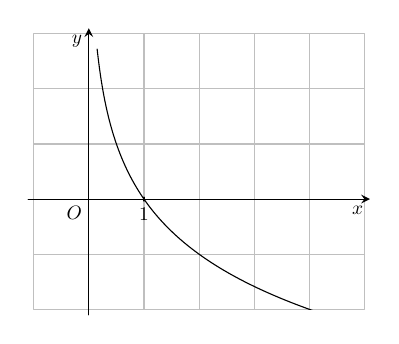
\begin{tikzpicture}[line join=round,line cap=round,>=stealth,scale=0.7]
				\draw[gray!50,xstep = 1,ystep = 1]  (-1,-2) grid (5,3);
				\draw[->]  (-1.1,0)--(5.1,0) node[below left] {$x$};
				\draw[->] (0,-2.1)--(0,3.1) node[below left] {$y$}; 
				\draw  (0,0) node [below left] {$O$};
				\foreach \x/\nx in {1/1} 
				\draw[thin]  (\x,1pt)--(\x,-1pt) node [below] {$\nx$};
				\begin{scope}
					 \clip (-1,-2) rectangle (5,3);
					 \draw[samples=200,domain=0.15:5,smooth,variable=\x] plot (\x,{ln((\x))/ln(0.5)});
				\end{scope}
			\end{tikzpicture}
		 }
	\loigiai{ 
		Hàm số xác định trên  $(0;+\infty)$.\\
		Hàm số nghịch biến trên  khoảng $(0;+\infty)$ nên cơ số $a\in (0;1)$.\\
		 Vậy hàm số $y=\log_{\tfrac{1}{2}}x$ có đồ thị như hình vẽ.
	 }
\end{ex}

% nguồn: Ok_TracNghiemLop11_Lan1
\begin{ex}%[1D6N3-3]%[ma:c5d9e559]
	Trong các hàm số dưới đây, hàm số  nào nghịch biến trên tập số thực $\mathbb{R}$.
	 \choice
		{$y=\left(\dfrac{\pi}{3}\right)^x$} 
		 {$y=\log_{\frac{\pi}{4}}\left(2x^2+1\right)$}
		{\True  $y=\left(\dfrac{2}{\mathrm{e}}\right)^x$}
		{$y=\log_{\frac{2}{3}}x$} 
	\loigiai{ 
		Vì  $\dfrac{2}{\mathrm{e}}<1$ nên $y=\left(\dfrac{2}{\mathrm{e}}\right)^x$ nghịch biến trên $\mathbb{R}$.\\
	 }
\end{ex}

% nguồn: Ok_TracNghiemLop11_Lan1
\begin{ex}%[1D6N3-3]%[ma:e6453663]
	Hàm số nào dưới đây đồng biến trên tập xác định  của nó?
	 \choice
		{$y=\left( \dfrac{1}{\pi}\right)^x$} 
		{$y=\left(  \dfrac{2}{3} \right)^x$}
		{\True $y=\left(  \sqrt{3} \right)^x$}
		{$y=\left(  0{,}5 \right)^x$}
	 \loigiai{
		Hàm  số $y=a^x$ đồng biến trên $\mathbb{R}$ khi và chỉ khi $a>1$.\\
	Thấy các số $\dfrac{1}{\pi};\dfrac{2}{3};0{,}5$ nhỏ hơn $1$,  còn $\sqrt{3}$ lớn hơn $1$ nên chọn $y=\left( \sqrt{3} \right)^x$.}
\end{ex}

% nguồn: Ok_TracNghiemLop11_Lan1
\begin{ex}%[1D6N3-3]%[ma:14cb49f0]
	Tìm hàm số đồng biến  trên $\mathbb{R}$.
	\choice 
		{\True  $f(x)=3^x$}
		{$f(x)=3^{-x}$} 
		{$f(x)=\left(\dfrac{1}{\sqrt{3}}\right)^x$} 
		{$f(x)=\dfrac{3}{3^x}$} 
	 \loigiai{
		Vì $3>1$ nên hàm số $f(x)=3^x$ đồng biến trên $\mathbb{R}$. 
	 }
\end{ex}

% nguồn: Ok_TracNghiemLop11_Lan1
\begin{ex}%[1D6N3-3]%[ma:6a280885]
	Hàm số nào sau đây  đồng biến trên $\mathbb{R}$?
	\choice 
		 {$y=10^{-x}$}
		{\True $y=\left(3-\sqrt{2}\right)^x$} 
		 {$y=\log_3x$}
		 {$y=\left(\dfrac{\pi}{2\mathrm{e}}\right)^x$}
	 \loigiai{
		Xét hàm số $y=\left(3-\sqrt{2}\right)^x$ có tập xác định trên  $\mathbb{R}$ và cơ số $a=\left(3-\sqrt{2}\right)>1$ nên hàm số đồng biến trên $\mathbb{R}$.
	 }
\end{ex}

% nguồn: Ok_TracNghiemLop11_Lan1
\begin{ex}%[1D6N3-3]%[ma:a475156f]
	Hàm số nào dưới đây đồng biến trên tập xác định của  nó?
	\choice 
		 {$y=\left(\dfrac{1}{\pi}\right)^x$}
		 {$y=\left(\dfrac{2}{3}\right)^x$}
		{\True $y=\left(\sqrt{3}\right)^x$} 
		 {$y=\left(0{,}5\right)^x$}
	 \loigiai{
		Hàm số $y=a^x$ đồng biến trên $\mathbb{R}$ khi và chỉ khi $a>1$.\\ 
		Thấy các số $\dfrac{1}{\pi}; \dfrac{2}{3}; 0{,}5$ nhỏ hơn $1$,  còn $\sqrt{3}$ lớn hơn $1$.\\
	Vậy hàm số  $y=\left(\sqrt{3}\right)^x$ đồng biến trên $\mathbb{R}$.}
\end{ex}

% nguồn: Ok_TracNghiemLop11_Lan1
\begin{ex}%[1D6N3-3]%[ma:7486788f]
	Đường cong  trong hình vẽ sau là đồ thị của hàm số nào dưới đây?
	\begin{center}
		\begin{tikzpicture}[scale=.8,>=stealth,font=\footnotesize,line join=round,line cap=round]
				\def\xmax{5} \def\ymin{-2.5} \def\ymax{3} 
				\pgfmathsetmacro{\e}{exp (1)} 
				\draw[->] (-0.9,0)--(\xmax,0) node [below]{$x$}; 
				\draw[->] (0,\ymin)--(0,\ymax) node [left]{$y$}; 
				\node  at (0,0) [below left]{$O$};
				\clip (-0.9,\ymin)  rectangle (\xmax-0.1,\ymax-0.1);
				\draw[smooth,samples=300,domain=0.03:\xmax] plot (\x,{ln(\x)}); 
				\draw[dotted] (\e,0)|-(0,1); 
				\fill  (1,0) circle (1pt) node [below] {$1$}
					(\e,0) circle (1pt) node [below] {$\mathrm{e}$} 
					(0,1) circle (1pt)  node [left] {$1$};
			\end{tikzpicture}
	\end{center}
	 \choice
		 {$y=-\mathrm{e}^{x}$}
		{$y=|\ln{x}|$} 
		{$\True y=\ln{x}$} 
		 {$y=\mathrm{e}^{x}$}
	 \loigiai{
		Đồ thị hàm số đi qua điểm $(\mathrm{e};1)$ và nằm cả trên và dưới trục  hoành nên chỉ có hàm số $y=\ln{x}$ thỏa mãn.
	} 
\end{ex}

% nguồn: Ok_TracNghiemLop11_Lan1
\begin{ex}%[1D6N3-3]%[5-CTST]%[ma:f7edebf3]
	Tìm hàm  số đồng biến trên $\mathbb{R}$.
	 \choice
		 {\True $f(x) = 3^x$}
		{$f(x) = 3^{-x}$} 
		 {$f(x) = \left(\dfrac{1}{\sqrt{3}} \right)^{x}$}
		{$f(x) = \dfrac{3}{3^x}$} 
	\loigiai{ 
		Hàm số $f(x) = a^x$ đồng biến trên $\mathbb{R}$ nếu $a > 1$.\\ 
		Do đó hàm số $fx) = 3^x$ là hàm số đồng biến trên $\mathbb{R}$. 
	 }
\end{ex}

% nguồn: Ok_Toan11_TracNghiem_Lan2
\begin{ex}%[1D6H3-3]%[ma:fee28ff8]
	Trong bốn  hàm số sau, hàm số nào nghịch biến trên $\mathbb{R}$?
	 \choice
		{$y=2\,022^x$} 
		 {$y=\left(\dfrac{2\,022}{2\,021} \right)^x$}
		 {$y=\log_{2\,022} x$}
		{\True $y=\left(\dfrac{2\,021}{2\,022}  \right)^x$}
	\loigiai{Hàm số $y = a^x$ nghịch biến  trên $\mathbb{R}$ khi $0 < a < 1$.}
\end{ex}

% nguồn: Ok_Toan11_TracNghiem_Lan2
\begin{ex}%[1D6H3-3]%[ma:6c0c0987]
	\immini{Đường cong trong hình bên là của đồ thị  hàm số nào sau đây?
	\choice 
		{$y=\log_2  x$}
		 {\True $y=(0{,}8)^x$}
		 {$y=\log_{0{,}4} x$}
		{$y=\left(\sqrt{2}\right)^x$}}{\begin{tikzpicture}[line join = round,line cap = round,>=stealth,font=\footnotesize,scale =0.8]
		 \def\a{0.8}
		\def\f (#1){(\a)^(#1)} 
		 \def\xmin{-5}
		 \def\xmax{5}
		\def\ymin{-1} 
		 \def\ymax{4}
		\draw[->]  (\xmin,0)--(\xmax,0) node[below] {\footnotesize $x$};
		\draw[->] (0,\ymin)--(0,\ymax) node[right] {\footnotesize  $y$};
		\draw (0,0)  node [below left] {\footnotesize $O$};
		\draw[thick,smooth,samples=200] plot[domain=\xmin:\xmax]  (\x,{\f (\x)});
		 \path
			(0,1) node[below left]{$1$}; 
		\fill (0,1) circle (1pt); 
	\end{tikzpicture}
		} 
	\loigiai{Dựa vào đồ thị, ta có  hàm số có tập xác định $\mathbb{R}$ và hàm số nghịch biến suy ra $y=(0{,}8)^x$.}
\end{ex}

% nguồn: Ok_Toan11_TracNghiem_Lan2
\begin{ex}%[1D6H3-3]%[ma:3227ef4e]
	Cho $a$, $b$, $c$ là ba số thực dương khác $1$. Đồ thị  hàm số $y=a^x$, $y=b^x$, $y=c^x$ được cho ở hình vẽ dưới đây. Mệnh nào nào sau đây đúng?
	\begin{center}
		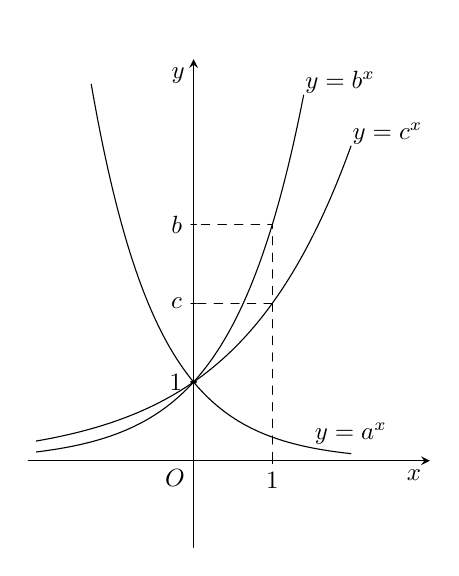
\begin{tikzpicture}[line join=round,line cap=round,>=stealth]
				\tikzset{every node/.style={scale=0.9}} 
				 \draw[->] (-2.1,0)--(3,0) node[below left] {$x$};
				\draw[->]  (0,-1.1)--(0,5.1) node[below left] {$y$};
				\draw (0,0) node [below left]  {$O$};
				\foreach \x/\nx  in {1/1}
				\draw[thin] (\x,1pt)--(\x,-1pt) node  [below] {$\nx$};
				\foreach \y/\ny  in {1/1,2/c,3/b}
				\draw[thin] (1pt,\y)--(-1pt,\y)  node [left] {$\ny$};
				 \draw[dashed,thin](1,2)--(0,2);
				\draw[dashed,thin](1,0)--(1,3)--(0,3); 
				\begin{scope}
					\clip (-2,-1)  rectangle (3,5.5);
					 \draw[samples=200,domain=-1.3:2,smooth,variable=\x] plot (\x,{0.3^(\x)}) node[above]{$y=a^x$};
					\draw[samples=200,domain=-2:1.4,smooth,variable=\x] plot (\x,{3^(\x)})  node[above right=-0.1cm]{$y=b^x$};
					 \draw[samples=200,domain=-2:2,smooth,variable=\x] plot (\x,{2^(\x)}) node[above right=-0.1cm]{$y=c^x$};
				\end{scope}
			\end{tikzpicture}
	\end{center}
	 \choice
		 {$a<b<c$}
		 {$b<c<a$}
		{$c<a<b$} 
		{\True  $a<c<b$}
	 \loigiai{
		Dựa vào đồ thị,  dễ thấy $\heva{&0<a<1\\&b,c>1.}$\\
		Đường thẳng  $x=1$ cắt hai đồ thị $y=b^x$, $y=c^x$ lần lượt tại $b$, $c$ và ta thấy $b>c$.\\
		Vậy $a<c<b$. 
	} 
\end{ex}

% nguồn: Ok_Toan11_TracNghiem_Lan2
\begin{ex}%[1D6H3-3]%[ma:51913cea]
	\immini{Đồ thị sau đây là đồ thị của  một trong bốn hàm số cho ở các phương án A, B, C, D. Hỏi đó là hàm số nào?
	 \choice
		{\True $y=\log_2  x$}
		 {$y=\dfrac{1}{2^x}$}
		{$y=\log_{\tfrac{1}{2}} x$} 
		{$y=2^x$}}{\begin{tikzpicture}[line join = round,line cap = round,>=stealth,font=\footnotesize,scale =1]
		 \def\a{2}
		\def\f (#1){ln (#1)/ln (\a)} 
		\def\xmin{-1} 
		\def\xmax{4} 
		 \def\ymin{-2.75}
		\def\ymax{3} 
		 \def\n{0.15}
		 \draw[->] (\xmin,0)--(\xmax,0) node[below] {\footnotesize $x$};
		\draw[->] (0,\ymin)--(0,\ymax) node[right] {\footnotesize $y$}; 
		\draw (0,0)  node [below left] {\footnotesize $O$};
		\draw[thick,smooth,samples=200] plot[domain= 
		\n:\xmax]  (\x,{\f (\x)});
		 \path (1,0) node[below]{$1$};
		\fill (1,0)  circle (1pt);
	\end{tikzpicture}
		 }
	 \loigiai{Hình dáng đồ thị đã cho là của hàm số logarit và đồ thị \lq\lq đi lên\rq\rq~ nên hàm số đồng biến.\\
	Vậy đồ thị trên  là của hàm số $y=\log_2 x$.}
\end{ex}

% nguồn: Ok_Toan11_TracNghiem_Lan2
\begin{ex}%[1D6H3-3]%[ma:0b4c4084]
	\immini{Đường cong trong hình bên là đồ thị của hàm số nào trong bốn hàm  số sau?
	 \choice
		{\True  $y=\log_2 x$}
		 {$y=\log_2 x^2$}
		{$y=\log_2 2x$} 
		{$y=\log_{\tfrac{1}{2}} x$}}{\begin{tikzpicture}[line join = round,line cap = round,>=stealth,font=\footnotesize,scale =1]
		 \def\a{2}
		 \def\f (#1){ln (#1)/ln (\a)}
		\def\xmin{-1} 
		\def\xmax{4} 
		\def\ymin{-3} 
		 \def\ymax{3}
		\def\n{0.13} 
		\draw[->] (\xmin,0)--(\xmax,0) node[below] {\footnotesize  $x$};
		\draw[->] (0,\ymin)--(0,\ymax)  node[right] {\footnotesize $y$};
		\draw (0,0)  node [below left] {\footnotesize $O$};
		\draw[thick,smooth,samples=200] plot[domain= 
		 \n:\xmax] (\x,{\f (\x)});
		\draw[dashed] (0.5,0)--(0.5,-1)--(0,-1); 
		\path (1,0)  node[below]{$1$}
			(0.5,0)  node[above]{$\tfrac{1}{2}$}
			(0,-1)  node[left]{$-1$};
		 \fill (1,0) circle (1pt)
			(0.5,-1)  circle (1pt);
	\end{tikzpicture}
		} 
	\loigiai{Dựa vào hình dạng đồ thị, loại  $y=\log_{\tfrac{1}{2}}x$.\\
		Do đồ thị hàm số đi qua điểm  $(1;0)$ nên loại đáp án $y=\log_2 2x$.\\
	Do đồ thị hàm số đi qua  điểm $\left(\dfrac{1}{2};-1 \right)$ nên loại đáp án $y=\log_2 x^2$.}
\end{ex}

% nguồn: Ok_Toan11_TracNghiem_Lan2
\begin{ex}%[1D6H3-3]%[ma:b17413b2]
	Hàm số  nào trong các hàm số sau đây đồng biến trên $(0;+\infty)$?
	\choice 
		{$y=\left(\sqrt{2}-1\right)^x$} 
		{\True $y=\log_9  x$}
		{$y=\left(0{,}6\right)^x$} 
		{$\log_{0{,}7}x$} 
	 \loigiai{Ta có $y=\log_9 x$ đồng biến trên $(0;+\infty)$, vì cơ số $a=9>1$.}
\end{ex}

% nguồn: Ok_Toan11_TracNghiem_Lan2
\begin{ex}%[1D6H3-3]%[ma:93e06ce5]
	\immini{Cho $a$, $b$, $c$ là ba số thực dương khác $1$. Đồ thị hàm số $y=a^x$, $y=b^x$, $y=c^x$ được cho ở hình vẽ dưới đây.  Mệnh nào nào sau đây đúng?
	\choice 
		 {$a<b<c$}
		 {$b<c<a$}
		{$c<a<b$} 
		{\True $a<c<b$}}{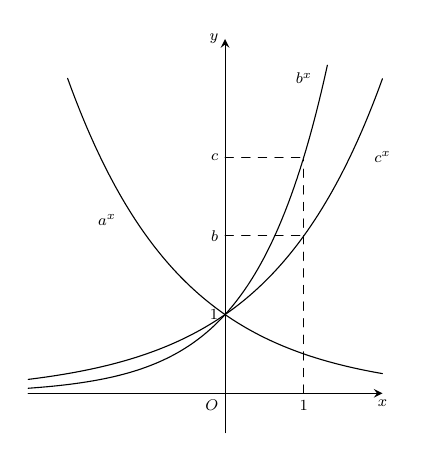
\begin{tikzpicture}[line join = round,line cap = round,>=stealth,font=\footnotesize,scale =1]
		 \draw[->] (-2.5,0) -- (2,0) node[below]{$x$};
		\draw[->] (0,-0.5)  -- (0,4.5) node[left]{$y$};
		 \node at (0,1) [left] {$1$};
		\node at (0,0) [below  left] {$O$};
		\node at (1,0) [below] {$1$}; 
		\node at (0,2) [left] {$b$}; 
		\node  at (0,3) [left] {$c$};
		\draw plot[domain=-2:2,samples=100] (\x,{pow  (0.5,\x)});
		\node at (-1.5,2.2) {$a^x$}; 
		 \draw plot[domain=-2.5:2,samples=100] (\x,{pow (2,\x)});
		\node at  (2,3) {$c^x$};
		\draw  plot[domain=-2.5:1.3,samples=100] (\x,{pow (3,\x)});
		\node at  (1,4) {$b^x$};
		\draw[dashed] (1,0) -- (1,3); 
		 \draw[dashed] (0,2) -- (1,2);
		\draw[dashed] (0,3) -- (1,3); 
	\end{tikzpicture}
		 }
	\loigiai{Dựa vào đồ thị, dễ thấy $\heva{&0<a<1 \\& b, c>1.}$\\ 
		Đường thẳng $x=1$ cắt hai đồ thị $y=b^x$, $y=c^x$ lần lượt tại hai điểm có tung độ  là $b$, $c$ và ta thấy $b>c$.\\
	Vậy $a<c<b$.} 
\end{ex}

% nguồn: Ok_Toan11_TracNghiem_Lan2
\begin{ex}%[1D6H3-3]%[ma:faa3a93a]
	Cho hàm số mũ $y=\left(6-a\right)^x$ với $a$ là tham  số. Có bao nhiêu số tự nhiên $a$ để hàm số đã cho đồng biến trên $\mathbb{R}$?
	\choice 
		{$3$} 
		{$6$} 
		 {\True $5$}
		{$4$} 
	\loigiai{Hàm số $y=\left(6-a\right)^x$  đồng biến trên $\mathbb{R} \Leftrightarrow 6-a>1 \Leftrightarrow a<5$.\\
		Mà $a \in \mathbb{N}  \Leftrightarrow a \in \left\{0;1;2;3;4\right\}$.\\
	Vậy có $5$ giá trị của $a$ thỏa mãn.} 
\end{ex}

% nguồn: Ok_Toan11_TracNghiem_Lan2
\begin{ex}%[1D6H3-3]%[ma:151b8732]
	\immini{Cho các hàm số $y=a^x$, $y=\log_b x$, $y=\log_c x$ có đồ thị  như hình vẽ bên. Chọn khẳng định đúng?
	 \choice
		 {$b>c>a$}
		 {$b>a>c$}
		{$a>b>c$} 
		{\True $c>b>a$}}{\begin{tikzpicture}[line join = round,line cap = round,>=stealth,font=\footnotesize,scale =1]
		\draw[->] (-2,0) --  (4,0) node[right] {$x$};
		\draw[->] (0,-2.5) --  (0,3) node[above] {$y$};
		\node  at (0,0) [below left] {$O$};
		\draw[domain=-0.8:4,samples=100,smooth] plot (\x,{pow  (0.3,\x)});
		\node  at (-1.5,2.1) {$y = a^x$};
		 \draw[domain=0.2:4,samples=100,smooth] plot (\x,{ln (\x)/ln (2)});
		\node at (2.5,2)  {$y = \log_b x$};
		\draw[domain=0.04:4,samples=100,smooth] plot (\x,{ln  (\x)/ln (4)});
		\node at (4,1.25) {$y = \log_c  x$};
	\end{tikzpicture}
		 }
	\loigiai{Hàm $y=a^x$ nghịch biến nên  $0<a<1$.\\
		Hàm $y=\log_b x$, $y=\log_c  x$ đồng biến nên $b$, $c>1$.\\
	Đường thẳng $y=1$ cắt đồ thị hàm số $y=\log_b x$,  $y=\log_c x$ tại các điểm có hoành độ lần lượt là $c$ và $b$. Ta thấy $b<c$.}
\end{ex}

% nguồn: Ok_Toan11_TracNghiem_Lan2
\begin{ex}%[1D6H3-3]%[ma:e528131e]
	\immini{Cho các hàm số $y=\log_a x$, $y=\log_b x$, $y=\log_c x$ có đồ thị như hình vẽ dưới đây. Chọn mệnh đề đúng. 
	\choice 
		{\True $a>c>b$} 
		{$a>b>c$} 
		 {$c>a>b$}
		{$b>c>a$}}{\begin{tikzpicture}[line join = round,line cap = round,>=stealth,font=\footnotesize,scale =1]
		\draw[->] (-0.5,0)  -- (5,0) node[right] {$x$};
		\draw[->] (0,-3) -- (0,3) node[above]  {$y$};
		\fill  (0,0) circle (1pt);
		\draw (1,0) circle (1pt); 
		\node[above]  at (1,0) {$1$};
		\draw[domain=0.14:5,samples=100] plot (\x,{ln  (\x)/ln (0.5)});
		\draw[domain=0.02:5,samples=100] plot  (\x,{ln (\x)/ln (4)});
		\draw[domain=0.13:5,samples=100] plot (\x,{ln  (\x)/ln (2)});
		\path  (5.25,1.15) node[right]{$y=\log_a x$}
			(5.25,2.5) node[right]{$y=\log_c x$} 
			(5.25,-2.25) node[right]{$y=\log_b  x$};
	\end{tikzpicture}
		} 
	\loigiai{\begin{center}
		\begin{tikzpicture}[line join = round,line cap = round,>=stealth,font=\footnotesize,scale =1]
				 \draw[->] (-0.5,0) -- (5,0) node[right] {$x$};
				\draw[->] (0,-3) --  (0,3) node[above] {$y$};
				 \fill (0,0) circle (1pt);
				 \draw (1,0) circle (1pt);
				\node[above] at (1,0)  {$1$};
				\draw[domain=0.14:5,samples=100] plot (\x,{ln (\x)/ln  (0.5)});
				\draw[domain=0.02:5,samples=100] plot (\x,{ln (\x)/ln  (4)});
				\draw[domain=0.13:5,samples=100] plot (\x,{ln (\x)/ln  (2)});
				\draw  (-0.5,1)--(5,1);
				\draw[dashed](2,1)--(2,0) 
					 (4,1)--(4,0);
				\path (5.25,1.15)  node[right]{$y=\log_a x$}
					(5.25,2.5)  node[right]{$y=\log_c x$}
					(5.25,-2.25) node[right]{$y=\log_b x$} 
					(-0.5,1) node[left]{$y=1$} 
					(2,1)  node[above]{$A$}
					(4,1) node[above]{$B$}; 
			\end{tikzpicture}
	\end{center}
	Dựa vào đồ thị ta có hàm số $y=\log_b x$ là một hàm số nghịch biến trên tập xác định của  nó nên $0 < b < 1$; hàm số $y=\log_a x$, $y=\log_c x$ là các hàm số đồng biến trên tập xác định của nó nên $a$, $c > 1$.\\
	Kẻ đường thẳng  $y=1$ cắt đồ thị hàm số $y=\log_c x$, $y=\log_a x$ lần lượt tại điểm $A(c;1)$ và $B(a;1)$.\\
Dựa  vào đồ thị ta thấy $x_A < x_B \Leftrightarrow c < a$.\\ Vậy $a>c>b$.}
\end{ex}

% nguồn: Ok_Toan11_TracNghiem_Lan2
\begin{ex}%[1D6H3-3]%[ma:bb7a46d2]
	Cho các hàm số $y=a^x$, $y=\log_bx$, $y=\log_cx$ có đồ thị như hình vẽ bên. Chọn  khẳng định đúng?
	\begin{center}
		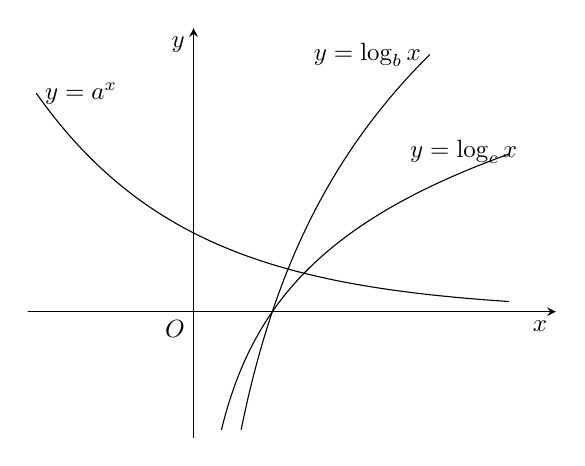
\begin{tikzpicture}[line join=round,line cap=round,>=stealth]
				 \tikzset{every node/.style={scale=0.9}}
				\draw[->] (-2.1,0)--(4.6,0) node[below left] {$x$}; 
				 \draw[->] (0,-1.6)--(0,3.6) node[below left] {$y$};
				\draw (0,0) node [below left] {$O$}; 
				\begin{scope}
					 \clip (-2,-1.5) rectangle (4.3,3.5);
					\draw[samples=200,domain=4:-2,smooth,variable=\x] plot  (\x,{0.6^(\x)}) node[right]{$y=a^x$};
					\draw[samples=200,domain=0.25:3,smooth,variable=\x] plot (\x,{ln ((\x))/ln  (1.4)}) node[left]{$y=\log_bx$};
					\draw[samples=200,domain=0.25:4,smooth,variable=\x] plot (\x,{ln ((\x))/ln  (2)}) node[above left=-0.25cm]{$y=\log_cx$};
				\end{scope}
			\end{tikzpicture}
	\end{center}
	 \choice
		{$b>c>a$} 
		{$b>a>c$} 
		 {$a>b>c$}
		 {\True $c>b>a$}
	 \loigiai{
		 Hàm $y=a^x$ nghịch biến nên $0<a<1$.\\
		Hàm $y=\log_bx$, $y=\log_cx$ đồng  biến nên $b$, $c>1$.\\
		Đường thẳng $y=1$ cắt đồ thị hàm số $y=\log_cx$, $y=\log_bx$ tại các điểm có hoành  độ lần lượt là $c$ và $b$. Ta thấy $b<c$.
	 }
\end{ex}

% nguồn: Ok_Toan11_TracNghiem_Lan2
\begin{ex}%[1D6H3-3]%[ma:b4afd773]
	 \immini{Cho hàm số $y=\log_a x$ ($a>0, a\neq 1$) có đồ thị như hình vẽ. Giá trị của $a$ bằng
	\choice 
		{$a=2$} 
		{\True  $a=\dfrac{1}{2}$}
		 {$a=\dfrac{1}{\sqrt{2}}$}
		{$a=\sqrt{2}$}}{\begin{tikzpicture}[line join = round,line cap = round,>=stealth,font=\footnotesize,scale =1]
		\def\a{0.5} 
		\def\f (#1){ln (#1)/ln (\a)} 
		 \def\xmin{-1}
		\def\xmax{4} 
		\def\ymin{-2.75} 
		\def\ymax{3} 
		 \def\n{0.15}
		\draw[->] (\xmin,0)--(\xmax,0) node[below] {\footnotesize $x$}; 
		\draw[->] (0,\ymin)--(0,\ymax) node[right] {\footnotesize $y$}; 
		\draw (0,0) node [below left]  {\footnotesize $O$};
		\draw[thick,smooth,samples=200]  plot[domain=
		\n:\xmax] (\x,{\f  (\x)});
		\draw[dashed]  (2,0)--(2,-1)--(0,-1);
		\path (1,0)  node[below]{$1$}
			 (2,0) node[above]{$2$}
			 (0,-1) node[left]{$-1$};
		 \fill (1,0) circle (1pt)
			(2,-1)  circle (1pt);
	\end{tikzpicture}
		 }
	\loigiai{Đồ thị hàm số $y=\log_a x$ đi qua điểm $(2;-1)$ nên $\log_a 2 =  -1$.\\
	Khi đó $a^{-1}=2\Leftrightarrow \dfrac{1}{a}=2 \Leftrightarrow a=\dfrac{1}{2}$.} 
\end{ex}

% nguồn: Ok_Toan11_TracNghiem_Lan2
\begin{ex}%[1D6H3-3]%[ma:1442da47]
	Hàm số nào  sau đây nghịch biến trên $\mathbb{R}$?
	\choice 
		{\True $y=\left(\dfrac{\pi}{4}\right)^x$} 
		{$y=\mathrm{e}^x$} 
		{$y=2\,022^x$} 
		{$y=2^x$} 
	\loigiai{Hàm số $y=\left(\dfrac{\pi}{4}\right)^x$ nghịch  biến trên $\mathbb{R}$ vì $0<\dfrac{\pi}{4}<1$.}
\end{ex}

% nguồn: Ok_Toan11_TracNghiem_Lan2
\begin{ex}%[1D6H3-3]%[ma:db7f5927]
	\immini{Cho các đồ thị hàm số $y=a^x$, $y=\log_b x$, $y=c^x$ ở hình  vẽ sau đây. Khẳng định nào sau đây đúng?
	\choice 
		 {$0<c<1<a<b$}
		{\True $c<0<a<1<b$} 
		 {$c<0<a<b<1$}
		{$0<c<a<b<1$}}{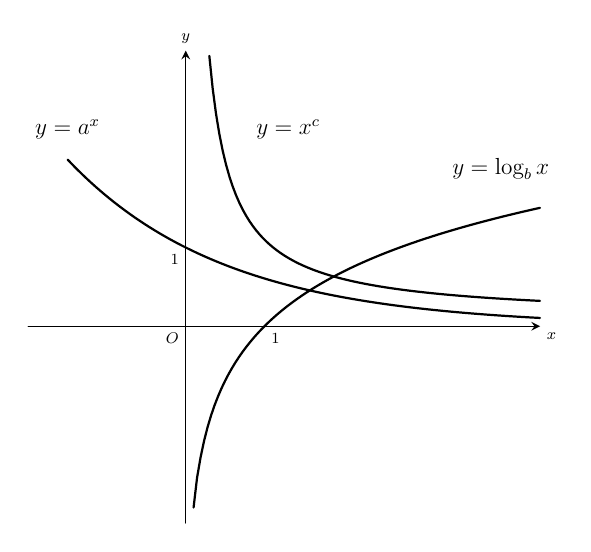
\begin{tikzpicture}[line join = round,line cap = round,>=stealth,font=\footnotesize,scale =1]
		\draw[->]  (-2,0) -- (4.5,0) node[below right] {$x$};
		\draw[->] (0,-2.5)  -- (0,3.5) node[above] {$y$};
		\node  at (0,0) [below left] {$O$};
		 \node at (0,1) [below left] {$1$};
		 \node at (1,0) [below right] {$1$};
		\draw[thick,domain=-1.5:4.5,samples=100]  plot (\x,{exp (-0.5*\x)});
		\node at (-1.5,2.5) {\large  $y=a^x$};
		\draw[thick,domain=0.3:4.5,samples=100]  plot (\x,{1/\x+0.1});
		\node  at (1.3,2.5) {\large $y=x^c$};
		\draw[thick,domain=0.1:4.5,samples=100]  plot (\x,{ln (\x)});
		\node at (4,2)  {\large $y=\log_b x$};
	\end{tikzpicture}
		} 
	\loigiai{Ta thấy đồ thị $y=x^c$ đi xuống nên $c<0$, đồ thị $y=a^x$ đi xuống nên  $0<a<1$, đồ thị $y=\log_b x$ đi lên nên $b>1$.}
\end{ex}

% nguồn: Ok_Toan11_TracNghiem_Lan2
\begin{ex}%[1D6H3-3]%[ma:4c74f9fa]
	Cho ba hàm  số $y=2^x$, $y=x$, $y=f(x)$ có đồ thị như hình bên, mệnh đề nào sau đây đúng?
	\begin{center}
		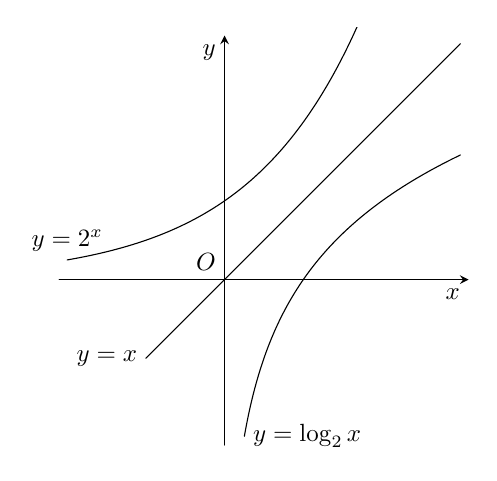
\begin{tikzpicture}[line join=round,line cap=round,>=stealth]
				\tikzset{every  node/.style={scale=0.9}}
				\draw[->] (-2.1,0)--(3.1,0) node[below left]  {$x$};
				\draw[->] (0,-2.1)--(0,3.1) node[below  left] {$y$};
				\draw (0,0)  node [above left] {$O$};
				\begin{scope}
					\clip  (-2.5,-2.2) rectangle (3,3.2);
					\draw[samples=200,domain=3:-2,smooth,variable=\x] plot  (\x,{2^(\x)}) node[above]{$y=2^x$};
					\draw[samples=200,domain=3:-1,smooth,variable=\x] plot  (\x,{1*(\x)}) node[left]{$y=x$};
					\draw[samples=200,domain=3:0.25,smooth,variable=\x] plot  (\x,{ln ((\x))/ln (2)}) node[right]{$y=\log_2x$};
				\end{scope}
			\end{tikzpicture}
	\end{center}
	 \choice
		 {$y=f(x)=\log_{\tfrac{1}{2}}x$}
		 {$y=f(x)=\ln x$}
		 {\True $y=f(x)=\log_2x$}
		 {$y=f(x)=\log x$}
	 \loigiai{
		Đồ thị hàm số $y=2^x$ và đồ thị hàm số $y=\log_2x$ đối xứng  nhau qua đường thẳng $y=x$.
	} 
\end{ex}

% nguồn: Ok_Toan11_TracNghiem_Lan2
\begin{ex}%[1D6H3-3]%[ma:bc497aa0]
	\immini{Đồ thị sau là đồ thị của hàm  số nào?
	 \choice
		 {$y=\log_2 x+1$}
		{$y=\log_2(x+1)  $}
		 {$y=\log_3 x$}
		{\True $y=\log_3(x+1) $}}{\begin{tikzpicture}[line join = round,line cap = round,>=stealth,font=\footnotesize,scale =1]
		 \def\a{3}
		\def\f (#1){ln (#1+1)/ln (\a)} 
		\def\xmin{-2} 
		\def\xmax{4} 
		 \def\ymin{-2.1}
		 \def\ymax{2}
		\def\n{-0.9} 
		\draw[->]  (\xmin,0)--(\xmax,0) node[below] {\footnotesize $x$};
		\draw[->] (0,\ymin)--(0,\ymax)  node[right] {\footnotesize $y$};
		\draw (0,0) node [below right] {\footnotesize $O$}; 
		\draw[thick,smooth,samples=200]  plot[domain=
		 \n:\xmax] (\x,{\f (\x)});
		 \draw[dashed] (2,0)--(2,1)--(0,1)
			(-1,\ymin)--(-1,\ymax); 
		\path (-1,0)  node[below left]{$-1$}
			 (2,0) node[below]{$2$}
			 (0,1) node[left]{$1$};
		\fill (1,2)  circle (1pt);
	\end{tikzpicture}
		} 
	 \loigiai{Dựa vào đồ thị, ta thấy\\
		Hàm số xác định trên  khoảng $(-1;+\infty)$ $\Rightarrow$ loại $y==\log_2 x+1$ và $y=\log_3 x$.\\
	Đồ thị hàm số đi qua điểm $(2;1)$.\\Vậy đồ thị đã cho  là hàm số $y=\log_3 (x+1)$.}
\end{ex}

% nguồn: Ok_Toan11_TracNghiem_Lan2
\begin{ex}%[1D6H3-3]%[ma:8530d9fd]
	\immini{Đồ thị  hình bên là đồ thị của hàm số nào?
	 \choice
		 {$y=2^x$}
		{$y=\left(\dfrac{1}{2}\right)^x$} 
		 {$y=\left(\dfrac{1}{3}\right)^x$}
		{\True $y=3^x$}}{\begin{tikzpicture}[line join = round,line cap = round,>=stealth,font=\footnotesize,scale =1]
		 \def\a{3}
		\def\f (#1){(\a)^(#1)} 
		 \def\xmin{-3}
		\def\xmax{2} 
		\def\ymin{-1} 
		\def\ymax{4} 
		\draw[->]  (\xmin,0)--(\xmax,0) node[below] {\footnotesize $x$};
		\draw[->] (0,\ymin)--(0,\ymax) node[right] {\footnotesize $y$}; 
		\draw (0,0) node  [below left] {\footnotesize $O$};
		\draw[thick,smooth,samples=200]  plot[domain=\xmin:1.2] (\x,{\f (\x)});
		 \draw[dashed] (1,0)--(1,3)--(0,3);
		\path (1,0) node[below]{$1$} 
			(0,3)  node[left]{$3$};
		\fill (1,3)  circle (1pt);
	\end{tikzpicture}
		} 
	\loigiai{Đồ thị hàm số \lq\lq đi lên\rq\rq~và qua điểm có tọa độ $(1;3)$ nên trong 4 phương án đã cho thì hàm số $y=3^x$  thỏa mãn được tính chất.}
\end{ex}

% nguồn: Ok_Toan11_TracNghiem_Lan2
\begin{ex}%[1D6H3-3]%[ma:657aa4dc]
	Đường cong trong hình bên là của đồ thị hàm số nào sau  đây?
	\begin{center}
		\begin{tikzpicture}[line join=round,line cap=round,>=stealth,scale=0.7]
				 \tikzset{every node/.style={scale=0.9}}
				\draw[->] (-6.1,0)--(6.1,0)  node[below left] {$x$};
				\draw[->] (0,-1.1)--(0,4.1) node[below  left] {$y$};
				\draw (0,0) node  [below left] {$O$};
				\begin{scope}
					\clip (-6,-1)  rectangle (6,4);
					\draw[samples=200,domain=-5.5:5.5,smooth,variable=\x] plot (\x,{0.8^(\x)}); 
				\end{scope}
			\end{tikzpicture}
	\end{center}
	\choice 
		{$y=\log_2x$} 
		{\True  $y=(0{,},8)^x$}
		 {$y=\log_{0{,}4}x$}
		{$y=(\sqrt  2)^x$}
	 \loigiai{
	Dựa vào đồ thị, ta có hàm số có tập xác định $\mathbb{R}$ và hàm  số nghịch biến suy ra $y=(0{,}8)^x$.}
\end{ex}

% nguồn: Ok_Toan11_TracNghiem_Lan2
\begin{ex}%[1D6H3-3]%[ma:26b7637f]
	Hàm số nào đồng biến trên toàn  tập xác định của nó?
	\choice 
		 {\True $y=\log_{\sqrt{2}} x$}
		{$y=\left(2\sqrt{2}\right)^{-x}$} 
		 {$y=\log_{\tfrac{1}{2}} x$}
		{$y=\left(\dfrac{\mathrm{e}}{\pi}\right)^{x}$} 
	\loigiai{Hàm số  $y=\log_{\sqrt{2}}x$ có cơ số $a=\sqrt{2}>1$ nên đồng biến trên tập xác định của nó là $(0;+\infty)$.\\
		Hàm số $y=\left(2\sqrt{2}\right)^{-x}=\left(\dfrac{1}{2\sqrt{2}}\right)^x$ có cơ số $0<a=\dfrac{1}{2\sqrt{2}}<1$ nên nghịch biến trên tập xác định  của nó là $\mathbb{R}$.\\
		Hàm số $y=\log_{\tfrac{1}{2}}x$ có cơ số $0<a=\dfrac{1}{2}<1$ nên nghịch biến  trên tập xác định của nó là $(0;+\infty)$.\\
	Hàm số $y=\left(\dfrac{\mathrm{e}}{\pi}\right)^x$ có cơ số $0<a=\dfrac{\mathrm{e}}{\pi}<1$ nên nghịch biến trên tập xác định của  nó là $\mathbb{R}$.}
\end{ex}

% nguồn: Ok_Toan11_TracNghiem_Lan2
\begin{ex}%[1D6H3-3]%[ma:7da53078]
	\immini{Đồ thị của hàm số sau là  đồ thị của hàm số nào?
	 \choice
		 {$y=x^2$}
		{$y=3^x$} 
		 {$y=\log_2 x$}
		{\True $y=2^x$}}{\begin{tikzpicture}[line join = round,line cap = round,>=stealth,font=\footnotesize,scale =1]
		 \def\a{2}
		\def\f (#1){(\a)^(#1)} 
		 \def\xmin{-3}
		 \def\xmax{3}
		\def\ymin{-1} 
		 \def\ymax{5}
		\draw[->] (\xmin,0)--(\xmax,0) node[below] {\footnotesize  $x$};
		\draw[->] (0,\ymin)--(0,\ymax) node[right] {\footnotesize $y$}; 
		 \draw (0,0) node [below left] {\footnotesize $O$};
		\draw[thick,smooth,samples=200] plot[domain=\xmin:2.2] (\x,{\f  (\x)});
		\draw[dashed] (2,0)--(2,4)--(0,4); 
		\path  (2,0) node[below]{$2$}
			(0,4)  node[left]{$4$}
			 (0,1) node[above left]{$1$};
		\fill (2,4) circle (1pt) 
			(0,1)  circle (1pt);
	\end{tikzpicture}
		} 
	\loigiai{Nhận thấy đồ thị hàm số đi qua hai điểm $(0;1)$ và  $(2;4)$, đối chiếu với các hàm số ta chọn hàm số $y = 2^x$.}
\end{ex}

% nguồn: Ok_Toan11_TracNghiem_Lan2
\begin{ex}%[1D6H3-3]%[ma:672d10ee]
	 \immini{Đồ thị bên là đồ thị của hàm số nào?
	\choice 
		 {$y=\log_2 x+1$}
		 {$y=\log_2(x+1) $}
		{$y=\log_3  x$}
		{\True $\log_3(x+1) $}}{\begin{tikzpicture}[line join = round,line cap = round,>=stealth,font=\footnotesize,scale =1]
		\draw[->] (-1.7,0) -- (4.2,0) node[below left]  {$x$};
		\draw[->] (0,-1) -- (0,2.5) node[above right]  {$y$};
		\node  at (0,0) [below right] {$O$};
		\node  at (0,1) [left] {$1$};
		\node at  (2,0) [below] {$2$};
		\node at (-1,0)  [below left] {$-1$};
		\draw  (-1,-1) -- (-1,2.5);
		\draw[smooth,domain=-0.65:4] plot (\x,{ln (\x+1)/ln (3)}); 
		\fill  (2,1) circle (1pt);
		 \draw[dashed] (2,1) -- (2,0);
		\draw[dashed]  (2,1) -- (0,1);
	\end{tikzpicture}
		 }
	\loigiai{Đồ  thị hàm số đi qua $(2;1)$, chọn hàm số $y = \log_3(x + 1)$.}
\end{ex}

% nguồn: Ok_Toan11_TracNghiem_Lan2
\begin{ex}%[1D6H3-3]%[ma:b2823deb]
	Hàm số nào sau đây luôn đồng biến trên  tập xác định?
	\choice 
		 {$y=0{,}3^x$}
		 {$y=\log_{\tfrac{1}{3}}x$}
		{\True $y=\log_{\tfrac{3}{2}}x$} 
		 {$y=\left(\dfrac{2}{3}\right)^x$}
	\loigiai{Ta có $\dfrac{3}{2} >  1$ suy ra hàm số $y=\log_{\tfrac{3}{2}}x$ đồng biến trên tập xác định của nó.}
\end{ex}

% nguồn: Ok_Toan11_TracNghiem_Lan2
\begin{ex}%[1D6H3-3]%[ma:cd7799bf]
	 Hàm số nào sau đây nghịch biến trên tập xác định của nó?
	 \choice
		{$y=\log_{\sqrt{3}}x$} 
		 {$y=\log_{2}x$}
		{\True $y=\log_{\tfrac{\mathrm{e}}{\pi}}x$} 
		{$y=\log_{\pi}x$} 
	\loigiai{Hàm số logarit $y=\log_{\tfrac{\mathrm{e}}{\pi}}x$ với cơ số $a=\dfrac{e}{\pi}$, $0 < a < 1$  là hàm số nghịch biến trên tập xác định, các hàm số logarit $y=\log_{\sqrt{3}}x$, $y=\log_{2}x$ và $y=\log_{\pi}x$ có cơ số lớn hơn $1$ là các hàm số đồng biến trên tập xác định của nó.}
\end{ex}

% nguồn: Ok_Toan11_TracNghiem_Lan2
\begin{ex}%[1D6H3-3]%[ma:4210bfe9]
	Trong hình vẽ dưới đây có đồ thị của các  hàm số $y=a^x$, $y=b^x$, $y=\log_cx$.
	\begin{center}
		\begin{tikzpicture}[line join=round,line cap=round,>=stealth]
				 \tikzset{every node/.style={scale=0.9}}
				\draw[->] (-3.1,0)--(5.1,0) node[below left]  {$x$};
				\draw[->] (0,-1.1)--(0,5.1)  node[below left] {$y$};
				\draw  (0,0) node [below left] {$O$};
				\foreach \y/\ny in  {1/1}
				\draw[thin] (1pt,\y)--(-1pt,\y) node  [left=0.1cm] {$\ny$};
				\begin{scope}
					\clip (-3,-1)  rectangle (5,5);
					\draw[samples=200,domain=-3:4.5,smooth,variable=\x] plot (\x,{0.6^(\x)}) node[above]{$y=a^x$}; 
					 \draw[samples=200,domain=-3:2.3,smooth,variable=\x] plot (\x,{2^(\x)}) node[below right]{$y=b^x$};
					 \draw[samples=200,domain=0.25:4.5,smooth,variable=\x] plot (\x,{ln ((\x))/ln (2)}) node[above]{$y=c^x$};
				\end{scope}
			\end{tikzpicture}
	\end{center}
	Mệnh đề nào sau đây  đúng?
	 \choice
		{$a<b<c$} 
		 {$a<b=c$}
		 {$b<c<a$}
		{\True $a<c<b$} 
	\loigiai{ 
		Hàm số $y=a^x$  nghịch biến trên $\mathbb{R}$ nên $0<a<1$.\\
		Các hàm số $y=b^x$, $y=\log_cx$ đồng biến biến trên tập xác định của nó  nên $b$, $c>1$.\\
		Suy ra  $0<a<b$, $c<1$.\\
		Xét  đồ thị hàm số $y=\log_cx$, ta có $\log_c2>1\Leftrightarrow c<2$.\\
		Xét đồ thị hàm số $y=b^x$, ta có  $b^1>2\Leftrightarrow b>2$.\\
		Do đó  $0<a<c<b$.
	 }
\end{ex}

% nguồn: Ok_Toan11_TracNghiem_Lan2
\begin{ex}%[1D6H3-3]%[ma:72a498ee]
	Hàm số nào trong các hàm số sau đây nghịch biến trên  $\mathbb{R}$?
	\choice 
		{$y=\log_{5}x$} 
		{$y=5^x$} 
		 {\True $y=(0{,}5)^x$}
		{$y=\log_{0{,}5}x$} 
	\loigiai{Hàm số $y=(0{,}5)^x$ nghịch biến trên $\mathbb{R}$ vì $0<0{,}5<1$.} 
\end{ex}

% nguồn: Ok_Toan11_TracNghiem_Lan2
\begin{ex}%[1D6H3-3]%[ma:782fdd2c]
	Cho các đồ thị hàm số $y=a^x$, $y=\log_bx$,  $y=x^c$ ở hình vẽ sau đây.
	\begin{center}
		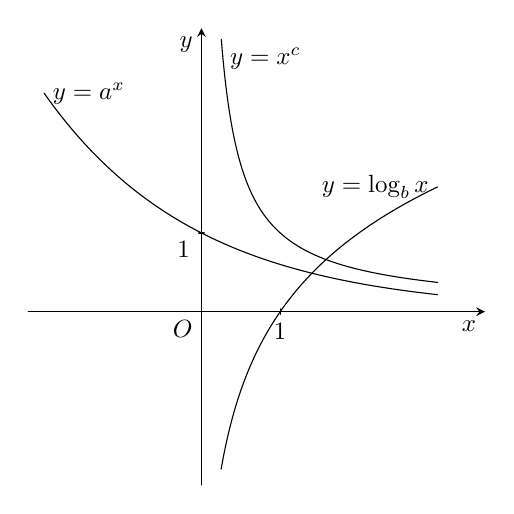
\begin{tikzpicture}[line join=round,line cap=round,>=stealth]
				\tikzset{every node/.style={scale=0.9}} 
				\draw[->] (-2.2,0)--(3.6,0) node[below  left] {$x$};
				\draw[->]  (0,-2.2)--(0,3.6) node[below left] {$y$};
				\draw (0,0) node [below left] {$O$}; 
				\foreach \x/\nx  in {1/1}
				\draw[thin] (\x,1pt)--(\x,-1pt) node  [below] {$\nx$};
				\foreach  \y/\ny in {1/1}
				\draw[thin] (1pt,\y)--(-1pt,\y) node  [below left] {$\ny$};
				\begin{scope}
					 \clip (-2.2,-2.2) rectangle (3.5,3.5);
					\draw[samples=200,domain=3:-2,smooth,variable=\x] plot  (\x,{0.6^(\x)}) node[right]{$y=a^x$};
					\draw[samples=200,domain=3:0.25,smooth,variable=\x] plot (\x,{(\x)^(-0.9)}) node[below  right]{$y=x^c$};
					\draw[samples=200,domain=0.25:3,smooth,variable=\x] plot (\x,{ln ((\x))/ln (2)})  node[left] {$y=\log_bx$};
				\end{scope}
			\end{tikzpicture}
	\end{center}
	Khẳng định nào sau  đây đúng?
	 \choice
		 {$0<c<1<a<b$}
		{\True  $c<0<a<1<b$}
		{$c<0<a<b<1$} 
		{$0<c<a<b<1$} 
	 \loigiai{
		Ta thấy đồ thị $y=x^c$ đi xuống nên  $c<0$, đồ thị $y=a^x$ đi xuống nên $0<a<1$, đồ thị $y=\log_bx$ đi lên nên $b>1$.
	 }
\end{ex}

% nguồn: Ok_Toan11_TracNghiem_Lan2
\begin{ex}%[1D6H3-3]%[ma:b13f1ba4]
	\immini{Cho đồ thị  hàm số $y=a^x$; $y=b^x$; $y=\log_c x$ như hình vẽ. Tìm mối liên hệ của $a, b, c$.
	\choice 
		{\True  $c < b < a$}
		{$b < a <  c$}
		{$a  < b < c$}
		{$c < a < b$}}{\begin{tikzpicture}[line join = round,line cap = round,>=stealth,font=\footnotesize,scale =1]
		\draw[->] (-1.5,0) --  (4,0) node[below] {$x$};
		\draw[->] (0,-1.5) -- (0,4.5) node[left]  {$y$};
		\node  at (0,0) {$O$};
		\fill (0,0)  circle (1pt);
		 \node[above left] at (0,1) {$1$};
		 \fill (0,1) circle (1pt);
		\node[below] at (1,0) {$1$}; 
		\fill (1,0) circle  (1pt);
		 \draw[smooth] plot[domain=-1.5:2.1,samples=100] (\x,{2^\x});
		\node at (1.5,4.5) {$y=a^x$}; 
		 \draw[smooth] plot[domain=-1.5:3,samples=100] (\x,{1.5^\x});
		\node at (3,2.2)  {$y=b^x$};
		\draw[smooth] plot[domain=0.02:4,samples=100] (\x,{ln (\x)/ln (0.4)}); 
		\node  at (3,-1.9) {$y=\log_c x$};
	\end{tikzpicture}
		 }
	\loigiai{Nhìn đồ thị ta thấy  hàm số $y = a^x$ là hàm số đồng biến nên $a > 1$; $y = b^x$ là hàm số đồng biến nên $b > 1$; $y = \log_c x$ là hàm số nghịch biến nên $0 < c < 1$ do vậy ta có $\heva{& 0 < c < a \\& 0 < c < b .}$\\
	Khi thay $x = 1$ vào hai hàm số  $y = a^x$; $y = b^x$ ta thu được $a > b$ vậy $c < b < a$.}
\end{ex}

% nguồn: Ok_Toan11_TracNghiem_Lan2
\begin{ex}%[1D6H3-3]%[ma:d7e3c34b]
	\immini{Trong hình vẽ bên có đồ thị của các hàm số $y=a^x$, $y=b^x$, $y=\log_c x$. Mệnh đề  nào sau đây đúng?
	 \choice
		{$a < b < c$} 
		{$a <  b=c$}
		{$b <  c < a$}
		{\True $a < c < b$}}{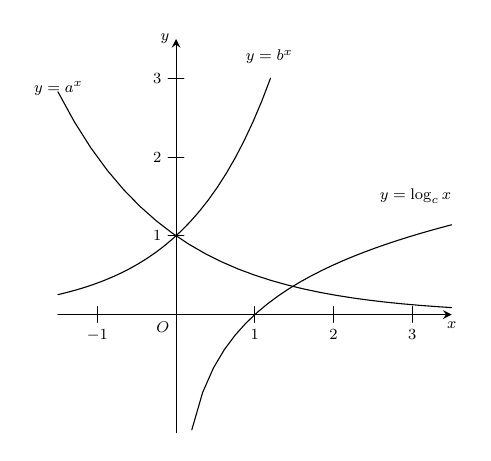
\begin{tikzpicture}[line join = round,line cap = round,>=stealth,font=\footnotesize,scale =1]
		 \draw[->] (-1.5,0) -- (3.5,0) node[below] {$x$};
		\draw[->] (0,-1.5) -- (0,3.5) node[left]  {$y$};
		\node at (0,0) [below left]{$O$}; 
		\foreach \x in {-1,1,2,3} 
		\draw  (\x,0.1) -- (\x,-0.1) node[below] {$\x$};
		\foreach \y in {1,2,3} 
		\draw (0.1,\y)  -- (-0.1,\y) node[left] {$\y$};
		 \draw[domain=-1.5:3.5] plot (\x,{(0.5)^\x});
		\node[above left] at (-1.1,2.7)  {$y = a^x$};
		 \draw[domain=-1.5:1.2] plot (\x,{(2.5)^\x});
		\node[above right] at (0.8,3.1) {$y = b^x$}; 
		\draw[domain=0.2:3.5] plot (\x,{ln (\x)/ln  (3)});
		\node[right]  at (2.5,1.5) {$y = \log_c x$};
	\end{tikzpicture}
		} 
	\loigiai{- Hàm số  $y=a^x$ nghịch biến trên $\mathbb{R}$ nên $0 < a < 1$.\\
		- Các hàm số $y=b^x$, $y=\log_c x$ đồng biến biến trên tập xác định của nó  nên $b$, $c > 1$.\\ Suy ra $0 < a < b, c < 1$.\\
		 - Xét đồ thị hàm số $y=\log_c x$, ta có $\log_c 2 > 1 \Leftrightarrow c < 2$.\\
	- Xét đồ thị hàm số $y=b^x$, ta có $b^1 >  2 \Leftrightarrow b > 2$. Do đó $0 < a < c < b$.}
\end{ex}

% nguồn: Ok_Toan11_TracNghiem_Lan2
\begin{ex}%[1D6H3-3]%[ma:335e47af]
	 Hàm số nào sau đây đồng biến trên $\mathbb{R}$?
	 \choice
		 {$y=\left(\dfrac{2}{5} \right)^x$}
		 {$y=\left(\dfrac{1}{3} \right)^x$}
		{\True $y=2005^x$} 
		{$y=2\,022$} 
	\loigiai{Ta có $y = 2\,005^x$ có $2\,005 > 1$ nên hàm số đồng biến  trên $\mathbb{R}$.}
\end{ex}

% nguồn: Ok_Toan11_TracNghiem_Lan2
\begin{ex}%[1D6H3-3]%[ma:1ea4c080]
	Tìm $a$ để đồ thị hàm số $y=\log_ax$, $(0<a\ne 1)$ có đồ thị  là hình bên.
	\begin{center}
		\begin{tikzpicture}[line join=round,line cap=round,>=stealth]
				\tikzset{every  node/.style={scale=0.9}}
				 \draw[->] (-1.1,0)--(4.1,0) node[below left] {$x$};
				\draw[->] (0,-1.1)--(0,4.1)  node[below left] {$y$};
				\draw (0,0) node [below left]  {$O$};
				 \foreach \x/\nx in {1/1,2/2}
				 \draw[thin] (\x,1pt)--(\x,-1pt) node [below] {$\nx$};
				\foreach  \y/\ny in {2/2}
				\draw[thin] (1pt,\y)--(-1pt,\y) node [left]  {$\ny$};
				 \draw[dashed,thin](2,0)--(2,2)--(0,2);
				\begin{scope}
					\clip (-1,-1) rectangle (4,4.5); 
					\draw[samples=200,domain=0.25:4,smooth,variable=\x]  plot (\x,{ln ((\x))/ln (sqrt (2))}) node[left]{$y=\log_ax$};
				\end{scope}
			\end{tikzpicture}
	\end{center}
	 \choice
		{\True $a=\sqrt{2}$} 
		{$a=\dfrac{1}{\sqrt{2}}$} 
		 {$a=\dfrac{1}{2}$}
		{$a=2$} 
	\loigiai{ 
		Do đồ thị hàm  số đi qua điểm $(2;2)$ nên $2=\log_a2\Leftrightarrow a=\sqrt 2$.
	 }
\end{ex}

% nguồn: Ok_Toan11_TracNghiem_Lan2
\begin{ex}%[1D6H3-3]%[ma:64b478a2]
	Cho $a$, $b$, $c$ là ba  số dương khác $1$. Đồ thị các hàm số $y=\log_ax$, $y=\log_bx$, $y=\log_cx$ như hình vẽ bên. Mệnh đề nào dưới đây là mệnh đề đúng?
	\begin{center}
		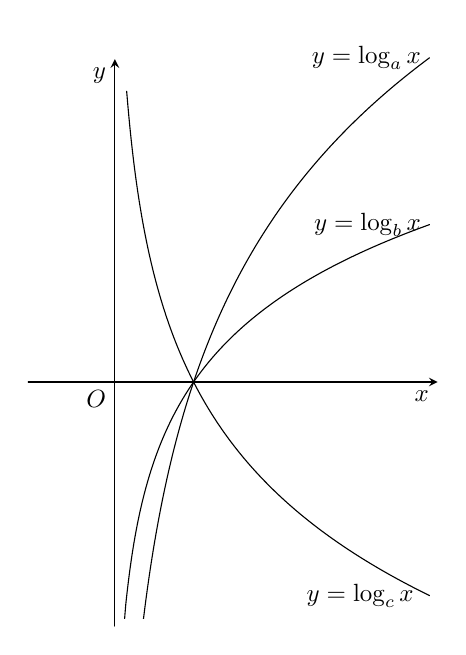
\begin{tikzpicture}[line join=round,line cap=round,>=stealth]
				\tikzset{every node/.style={scale=0.9}} 
				\draw[->] (-1.1,0)--(4.1,0) node[below  left] {$x$};
				\draw[->] (0,-3.1)--(0,4.1)  node[below left] {$y$};
				\draw  (0,0) node [below left] {$O$};
				\begin{scope}
					\clip (-1,-3) rectangle  (4,4.5);
					\draw[samples=200,domain=0.25:4,smooth,variable=\x]  plot (\x,{ln ((\x))/ln (1.4)}) node[left]{$y=\log_ax$};
					\draw[samples=200,domain=0.1:4,smooth,variable=\x] plot (\x,{ln ((\x))/ln (2)})  node[left]{$y=\log_bx$};
					\draw[samples=200,domain=0.15:4,smooth,variable=\x] plot (\x,{ln ((\x))/ln  (0.6)}) node[left=0.1cm]{$y=\log_cx$};
				\end{scope}
			\end{tikzpicture}
	\end{center}
	\choice 
		 {$a<b<c$}
		 {$b<c<a$}
		 {\True $c<a<b$}
		{$c<b<a$} 
	 \loigiai{
		 Dựa vào đồ thị, ta có $0<c<1$; $a>1$; $b>1$ và $\forall x>1$; $\log_ax>\log_bx$ nên $1<a<b$.\\
		Vậy $c<a<b$. 
	 }
\end{ex}

% nguồn: Ok_Toan11_TracNghiem_Lan2
\begin{ex}%[1D6H3-3]%[ma:f34e8540]
	Cho đồ thị hàm số $y=a^x$; $y=b^x$; $y=\log_cx$ như hình vẽ. Tìm mối liên  hệ của $a$, $b$, $c$.
	\begin{center}
		\begin{tikzpicture}[line join=round,line cap=round,>=stealth]
				\tikzset{every node/.style={scale=0.9}} 
				 \draw[->] (-1.1,0)--(4.1,0) node[below left] {$x$};
				 \draw[->] (0,-1.1)--(0,4.1) node[below left] {$y$};
				\draw  (0,0) node [below left] {$O$};
				\foreach \x/\nx in {1/1} 
				\draw[thin] (\x,1pt)--(\x,-1pt) node [below] {$\nx$}; 
				\foreach \y/\ny  in {1/1}
				\draw[thin]  (1pt,\y)--(-1pt,\y) node [above left] {$\ny$};
				\begin{scope}
					\clip (-1,-1.5) rectangle  (5,4.1);
					 \draw[samples=200,domain=-1:1.5,smooth,variable=\x] plot (\x,{2.5^(\x)}) node[right]{$y=a^x$};
					\draw[samples=200,domain=-1:3.3,smooth,variable=\x] plot (\x,{1.5^(\x)})  node[right]{$y=b^x$};
					\draw[samples=200,domain=0.089:2.8,smooth,variable=\x] plot (\x,{ln ((\x))/ln (0.4)})  node[above right=-0.1cm]{$y=c^x$};
				\end{scope}
			\end{tikzpicture}
	\end{center}
	\choice 
		 {\True $c<b<a$}
		{$b<a<c$} 
		 {$a<b<c$}
		 {$c<a<b$}
	 \loigiai{
		Nhìn đồ thị ta thấy hàm số  $y=a^x$ là hàm số đồng biến nên $a>1$; $y=b^x$ là hàm số đồng biến nên $b>1$; $y=\log_cx$ là hàm số nghịch biến nên $0<c<1$ do vậy ta có $\heva{&0<c<a\\&0<c<b.}$\\
		Khi thay $x=1$ vào hai hàm số $y=a^x$;  $y=b^x$ ta thu được $a>b$ vậy $c<b<a$.
	} 
\end{ex}

% nguồn: Ok_Toan11_TracNghiem_Lan2
\begin{ex}%[1D6H3-3]%[ma:a31547ca]
	 \immini{Cho đồ thị hàm số $y=f(x)$ như hình vẽ bên. Hàm số $y=f(x)$ có thể là hàm số nào dưới đây?
	 \choice
		{$y=\mathrm{e}^{-x}$} 
		{\True $y=\log  x$}
		{$y=-\ln x$} 
		{$y=e^x$}}{\begin{tikzpicture}[line join = round,line cap = round,>=stealth,font=\footnotesize,scale =1]
		\def\a{10} 
		\def\f  (#1){ln (#1)/ln (\a)}
		 \def\xmin{-1}
		 \def\xmax{4}
		 \def\ymin{-2}
		\def\ymax{2} 
		\def\n{0.01} 
		 \draw[->] (\xmin,0)--(\xmax,0) node[below] {\footnotesize $x$};
		 \draw[->] (0,\ymin)--(0,\ymax) node[right] {\footnotesize $y$};
		\draw  (0,0) node [below left] {\footnotesize $O$};
		\draw[thick,smooth,samples=200]  plot[domain=
		\n:\xmax]  (\x,{\f (\x)});
		\path (1,0) node[below]{$1$}; 
		\fill  (1,0) circle (1pt);
	\end{tikzpicture}
		} 
	\loigiai{Nhận xét  hàm số $y=f(x)$ có miền giá trị là $\mathbb{R}$ nên ta loại phương án $y=\mathrm{e}^{-x}$ và $y=\mathrm{e}^x$.\\
	Mặt khác quan sát đồ thị hàm số $y=f(x) \Rightarrow  f'(x) >0$ nên $y=\log x$.}
\end{ex}

% nguồn: Ok_Toan11_TracNghiem_Lan2
\begin{ex}%[1D6H3-3]%[ma:8350c8b5]
	Trong các hàm số dưới đây, hàm số nào  nghịch biến trên $\mathbb{R}$?
	 \choice
		 {\True $y=\left(\sqrt{5}-2\right)^x$}
		{$y=\sqrt{\pi^x}$} 
		{$y=2021^x$} 
		{$y=\mathrm{e}^x$} 
	\loigiai{Ta có $0 < \sqrt{5}-2 < 1$ nên hàm số $y=\left(\sqrt{5}-2\right)^x$ nghịch  biến trên $\mathbb{R}$.}
\end{ex}

% nguồn: Ok_Toan11_TracNghiem_Lan2
\begin{ex}%[1D6H3-3]%[ma:294ac1b8]
	\immini{Hình bên là đồ  thị của hàm số nào trong các hàm số sau đây?
	 \choice
		{\True $y=(0{,}4)^x$} 
		{$y=(\sqrt{2})^x$} 
		{$y=\log_2  x$}
		{$y=\log_{0{,}4} x$}}{\begin{tikzpicture}[line join = round,line cap = round,>=stealth,font=\footnotesize,scale =1]
		 \def\a{0.4}
		\def\f  (#1){(\a)^(#1)}
		\def\xmin{-3} 
		\def\xmax{3} 
		 \def\ymin{-1}
		\def\ymax{4} 
		\draw[->] (\xmin,0)--(\xmax,0) node[below] {\footnotesize $x$}; 
		\draw[->] (0,\ymin)--(0,\ymax)  node[right] {\footnotesize $y$};
		\draw  (0,0) node [below left] {\footnotesize $O$};
		\draw[thick,smooth,samples=200]  plot[domain=-1.5:\xmax] (\x,{\f (\x)});
		\path 
			(0,1) node[above right]{$1$}; 
		 \fill
			(0,1) circle  (1pt);
	\end{tikzpicture}
		} 
	 \loigiai{Hình bên là đồ thị của hàm mũ có cơ số $a$ thỏa $0 < a < 1$.}
\end{ex}

% nguồn: Ok_Toan11_TracNghiem_Lan2
\begin{ex}%[1D6H3-3]%[ma:828b8746]
	 Hàm số nào sau đây đồng biến trên $\mathbb{R}$?
	 \choice
		 {$y=\left(2-\sqrt{2}\right)^x$}
		 {$y=\left(\sqrt{3}-1\right)^x$}
		{\True $y=\left(\dfrac{\pi}{3}\right)^x$} 
		{$y=\left(\dfrac{\mathrm{e}}{4}\right)^x$} 
	\loigiai{Xét hàm số $y=\left(\dfrac{\pi}{3}\right)^x$ với $a=\dfrac{\pi}{3} > 1$ nên  hàm số $y=\left(\dfrac{\pi}{3}\right)^x$ đồng biến trên $\mathbb{R}$.}
\end{ex}

% nguồn: Ok_TracNghiemLop11_Lan1
\begin{ex}%[1D6H3-3]%[ma:3b298901]
	 \immini{
	Đường cong ở  hình bên là đồ thị của hàm số nào
	\choice 
		{$y=2^x$} 
		 {$y=\log_2 x$}
		 {$y=\left(\dfrac{1}{2}\right)^x$}
		{\True $y=\log_{\frac{1}{2}}  x$}
		 }{
		\begin{tikzpicture}[>=stealth,scale=0.7,line join=round,line cap=round]
				\def\xmax{3}  \def\ymin{-1} \def\ymax{2}
				 \draw[->] (-0.5,0)--(\xmax,0) node [below]{$x$};
				 \draw[->] (0,\ymin)--(0,\ymax) node [left]{$y$};
				\node at  (0,0) [below left]{$O$};
				\clip (-0.9,\ymin)  rectangle (\xmax-0.1,\ymax-0.1);
				\draw[smooth,samples=300,domain=0.3:2] plot (\x,{ln(\x)/ln(0.5)}); 
			\end{tikzpicture}
		} 
	\loigiai{Quan sát hình dáng đồ thị ta thấy đồ thị nằm bên phải trục $Oy$, đồ thị  đi xuống từ trái sang phải .
	} 
\end{ex}

% nguồn: Ok_TracNghiemLop11_Lan1
\begin{ex}%[1D6H3-3]%[ma:4a9a928d]
	Trong hình vẽ bên có đồ thị các hàm số  $y=a^x$, $y=b^x$, $y=\log_cx$. Hãy chọn mệnh đề đúng trong các mệnh đề sau đây?
	\begin{center}
		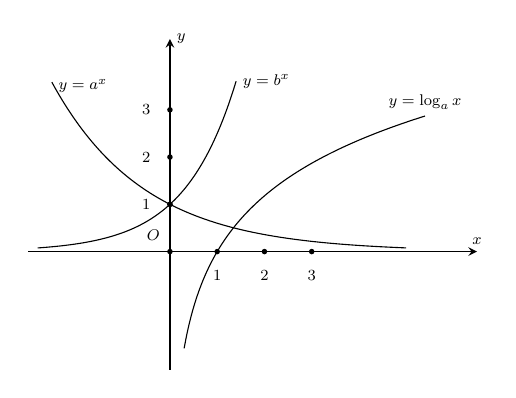
\begin{tikzpicture}[scale=1,>=stealth,font=\footnotesize,line join=round,line cap=roundm,x=0.6cm,y=0.6cm]
				\def \xmin{-3}; 
				\def  \xmax{6.5};
				\def \ymin{-2.5}; 
				\def \ymax{4.5}; 
				\draw[->] (\xmin,0) --  (\xmax,0) node[above] {$x$};
				\draw[->] (0.,\ymin) -- (0.,\ymax)  node[right] {$y$};
				\draw[smooth,samples=100,domain=-2.5:5] plot (\x,{(0.6^(\x))}); 
				\draw[smooth,samples=100,domain=-2.8:1.4] plot (\x,{(2.5^(\x))})  node[right]{$y=b^x$};
				\draw[smooth,samples=100,domain=0.3:5.4] plot (\x,{(ln(\x))/(ln(1.8))})  node[above]{$y=\log_ax$};
				\draw  (-2.5,3.5) node[right]{$y=a^x$};
				 \foreach \x/\y/\l/\g in {0/0/O/135,0/1/1/180,1/0/1/-90,0/1//0,0/2/2/180,0/3/3/180,2/0/2/-90,3/0/3/-90}{\fill[black] (\x,\y) circle (1pt)+(\g:0.5) node{$\l$};}
			\end{tikzpicture}
	\end{center}
	\choice 
		{\True $a < c  < b$}
		{$c  < a < b$}
		{$a < b=c$} 
		{$b <  c < a$}
	\loigiai{ 
		Hàm số $y=a^x$ nghịch biến  trên $\mathbb{R}$ nên ta có $0 < a < 1$.\\
		Các hàm số $y=b^x$, $y=\log_cx$ đồng  biến biến trên tập xác định của nó nên ta có $\heva{&b > 1\\&c > 1.}$\\
		Xét đồ thị hàm số $y=\log_cx$, ta có $\log_c2 > 1\Leftrightarrow c  < 2$.\\
		Xét đồ thị hàm số $y=b^x$, ta có $b^1> 2\Leftrightarrow b > 2$.\\ 
		Do đó $0 <  a < c < b$.
	} 
\end{ex}

% nguồn: Ok_TracNghiemLop11_Lan1
\begin{ex}%[1D6H3-3]%[ma:0a59667f]
	\immini{Hàm số  nào sau đây có đồ thị như hình bên?
	 \choice
		 {$y=\log_3x$}
		 {$y=\log_2x+1$}
		{\True  $y=\log_2(x+1)$}
		{$y=\log_3(x+1)$} 
		}{\begin{tikzpicture}[scale=1,font=\footnotesize,line join=round,line cap=round,>=stealth,x=0.6cm,y=0.6cm,declare function = {f (\x) =ln((\x)+1)/ln(2);}]
		\def  \xmin{-1.5};
		 \def \xmax{3.7};
		\def \ymin{-1.5}; 
		 \def \ymax{2.7};
		\draw[->] (\xmin,0.) -- (\xmax,0.) node[anchor=north]  {$x$};
		 \draw[->] (0.,\ymin) -- (0.,\ymax) node[anchor=west] {$y$};
		\clip (\xmin+0.1,\ymin+0.1) rectangle (\xmax-0.1,\ymax-0.1); 
		\draw[smooth,samples=100,domain=-0.9:\xmax]  plot (\x,{f (\x)});
		\draw[dashed]  (1,0) node[below]{$1$} |- (0,1) node[left]{$1$};
		\foreach \x/\y/\l/\g in {0/0/O/135,1/1//0,1/0//0,0/1//0}{\fill[black] (\x,\y) circle  (1pt)+(\g:0.5) node{$\l$};}
	\end{tikzpicture}
		} 
	\loigiai{ 
		Đồ thị trong hình vẽ  đi qua điểm $(0;0)$ và $(1;1)$.\\
		Trong $4$ phương án  chỉ có hàm số $y=\log_2 (x+1)$ có đồ thị phù hợp.
	} 
\end{ex}

% nguồn: Ok_TracNghiemLop11_Lan1
\begin{ex}%[1D6H3-3]%[ma:6e8b99ca]
	Cho các hàm số $y=\log_ax$ và $y=\log_bx$ có đồ thị như hình vẽ  bên.
	\begin{center}
		\begin{tikzpicture}[scale=1,>=stealth,font=\footnotesize,line join=round,line cap=roundm,x=0.6cm,y=0.6cm]
				 \def \xmin{-1.5};
				\def  \xmax{8.5};
				 \def \ymin{-2.5};
				 \def \ymax{3.5};
				\draw[->] (\xmin,0) -- (\xmax,0) node[above] {$x$}; 
				\draw[->] (0.,\ymin) -- (0.,\ymax)  node[right] {$y$};
				\draw[smooth,samples=100,domain=0.2:6.4]  plot (\x,{(ln(\x))/(ln(2))}) node[right]{$y=\log_bx$};
				\draw[smooth,samples=100,domain=0.2:6.4] plot (\x,{(ln(\x))/(ln(3))}) node[right]{$y=\log_ax$}; 
				\draw[dashed] (6,0)--(6,2.58); 
				 \foreach \x/\y/\l/\g in {0/0/O/135,1/0//0,6/2.58/C/120,6/1.63/B/120,6/0/A/120}{\fill[black] (\x,\y) circle (1pt)+(\g:0.5) node{$\l$};}
			\end{tikzpicture}
	\end{center}
	Đường thẳng $x=6$ cắt trục hoành, đồ thị hàm số $y=\log_ax$ và $y=\log_bx$ lần lượt tại $A$, $B$ và  $C$. Nếu $AC=AB{\log_2}3$ thì
	\choice 
		 {$b^3=a^2$}
		{$b^2=a^3$} 
		{$\log_3b=\log_2a$} 
		 {\True $\log_2b=\log_3a$}
	\loigiai{ 
		Từ các đồ thị hàm số đã  cho trên hình ta có $A(6;0)$, $B\left(6;\log_a6\right)$, $C\left(6;\log_b6\right)$.\\
		 $AC=y_C-y_A=\log_b6$, $AB=y_B-y_A=\log_a6$.\\
		Suy  ra
		\allowdisplaybreaks 
		\begin{eqnarray*}
			&&AC=AB\log_2 3\\ 
			&\Leftrightarrow& \log_b 6=\log_a6\cdot\log_23\\ 
			 &\Leftrightarrow& \dfrac{1}{\log_6b}=\dfrac{1}{\log_6a}\cdot\dfrac{\log_63}{\log_62}\\
			&\Leftrightarrow&  \dfrac{\log_62}{\log_6b}=\dfrac{\log_63}{\log_6a}\\
			&\Leftrightarrow& \log_2 b=\log_3a. 
		\end{eqnarray*}
	} 
\end{ex}

% nguồn: Ok_TracNghiemLop11_Lan1
\begin{ex}%[1D6H3-3]%[ma:2a93576b]
	\immini{Cho ba số thực dương $a$, $b$, $c$ khác $1$. Đồ thị các hàm số $y=a^x$,  $y=b^x$, $y=c^x$ được cho trong hình vẽ bên. Mệnh đề nào dưới đây đúng?
	\begin{center}
		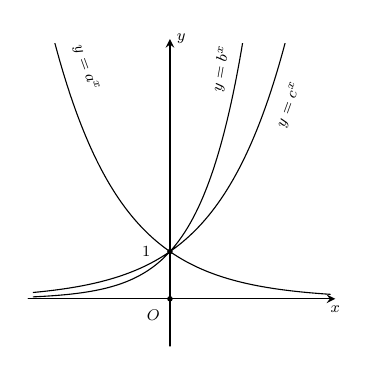
\begin{tikzpicture}[scale=1,font=\footnotesize,line join=round,line cap=round,>=stealth,x=0.6cm,y=0.6cm,declare function={f (\x)=2^(\x); g (\x)=3^(\x); h (\x)=0.5^(\x);}]
				\def \xmin{-3.0}; 
				\def \xmax{3.5}; 
				\def \ymin{-1.0}; 
				 \def \ymax{5.5};
				\draw[->] (\xmin,0.) -- (\xmax,0.)  node[anchor=north] {$x$};
				 \draw[->] (0.,\ymin) -- (0.,\ymax) node[anchor=west] {$y$};
				\clip  (\xmin+0.1,\ymin+0.1) rectangle (\xmax-0.1,\ymax-0.1);
				\draw[smooth,samples=100,domain=\xmin:\xmax] plot (\x,{f (\x)}) plot (\x,{g (\x)})  plot (\x,{h (\x)});
				 \draw (-2,\ymax) node[right,rotate=-70]{$y=a^x$}
					(1.2,\ymax)  node[left,rotate=80]{$y=b^x$}
					(2.3,\ymax-2)  node[right,rotate=70]{$y=c^x$};
				\foreach \x/\y/\l/\g in {0/0/O/225,0/1/1/180}{\fill[black] (\x,\y)  circle (1pt)+(\g:0.5) node{$\l$};}
			\end{tikzpicture}
	\end{center}
	\choice 
		{$a < b < c$} 
		 {\True $a < c < b$}
		{$b < c <  a$}
		{$c  < a < b$}}{x}
	 \loigiai{
		Từ đồ thị suy ra  $0 < a < 1$;\\
		$b > 1$, $c > 1$ và $b^x>c^x$ khi $x > 0$ nên $b  > c$.\\
		Vậy $a  < c < b$.
	} 
\end{ex}

% nguồn: Ok_TracNghiemLop11_Lan1
\begin{ex}%[1D6H3-3]%[ma:45e7c50e]
	\immini 
	 {
	Đường  cong trong hình bên là đồ thị của hàm số nào sau đây?
	 \choice
		{$y=\log  _2(2 x)$}
		 {$y=\log _{\tfrac{1}{2}}x$}
		{$y=\log _{\sqrt{2}}x$} 
		{\True $y=\log _2  x$}
		 }
		 {
		\begin{tikzpicture}[>=stealth,scale=0.7]
				\def\xmax{3} \def\xmin{-1}  \def\ymax{2} \def\ymin{-3.5}
				\draw[->] (\xmin,0) -- (\xmax,0) node[below]{\footnotesize $x$}; 
				\draw[->] (0,\ymin) --  (0,\ymax) node[left] {\footnotesize $y$};
				\draw (0,0) node[below left]{\footnotesize $O$}; \fill (0,0)  circle (1pt);
				\foreach  \x in{}
				\draw[shift={(\x,0)}]  (0,-2pt)--(0,2pt) node[below]{\footnotesize $\x$};
				 \foreach \y in{1}
				\draw[shift={(0,\y)}] (-2pt,0)--(2pt,0) node[left]{\footnotesize $\y$}; 
				\foreach \y in{-1} 
				\draw[shift={(0,\y)}] (-2pt,0)--(2pt,0) node[left]{\footnotesize  $\y$};
				 \draw[smooth,domain=0.1:3]plot (\x,{ln(\x)/ln(2)}) node[above] {};
				\foreach \x/\y in{0.5/-1}{\fill (\x,\y) circle (1pt); \draw[dashed](\x,0)--(\x,\y)--(0,\y);} 
				\draw (0.5,0) node[above]{\footnotesize  $\dfrac{1}{2}$};
			\end{tikzpicture}
		} 
	\loigiai{ 
		Đồ thị hàm số $y=\log  _2 x$.
	} 
\end{ex}

% nguồn: Ok_TracNghiemLop11_Lan1
\begin{ex}%[1D6H3-3]%[ma:2129bb28]
	Mệnh đề nào trong các  mệnh đề dưới đây \textbf{sai}?
	 \choice
		{Hàm số  $y=\left(\dfrac{2018}{\pi}\right)^x$ đồng biến trên $\mathbb{R}$}
		 {Hàm số $y=\log x$ đồng biến trên $\left(0;+\infty\right)$}
		{\True Hàm số $y=\ln \left(- x\right)$ nghịch biến trên khoảng $\left(-  \infty; 0\right)$}
		{Hàm số $y=2^x$  đồng biến trên $\mathbb{R}$}
	\loigiai{ 
		Hàm số $y=\ln(-x)$ có tập xác  định $\mathscr{D}=\left(- \infty; 0\right)$.\\
		Cơ số $a=\mathrm{e}>1$ do đó hàm số đồng  biến trên $\left(- \infty; 0\right)$.\\
	 }
\end{ex}

% nguồn: Ok_TracNghiemLop11_Lan1
\begin{ex}%[1D6H3-3]%[ma:6d2bb287]
	\immini[thm]{Hàm số  nào sau đây có đồ thị như hình bên?
	 \choice
		{$y=\log_3  x$}
		 {$y=\log_2 x+1$}
		{\True$y=\log_2 \left(x+1\right)$} 
		{$y=\log_3  \left(x+1\right)$}}
		{TIKZBLOCK100 
		} 
	 \loigiai{
		Nhìn hình ta thấy đồ thị đi qua điểm $M(1;1)$ và chỉ có hàm số  $y=\log_{2}(x+1)$ có đồ thị thỏa mãn.
	} 
\end{ex}

% nguồn: Ok_TracNghiemLop11_Lan1
\begin{ex}%[1D6H3-3]%[ma:97660b9c]
	Giá  trị của tham số $m$ để hàm số $y=\log_{(m+1)^2} x$ nghịch biến trên tập xác định của nó là
	\choice 
		 {$m \in(-\infty;0) \setminus\{-2;-1\}$}
		 {$m \in(-\infty;0) \setminus\{-1\}$}
		{$m \in(-2;0)$} 
		{\True $m \in(-2;0) \setminus\{-1\}$} 
	\loigiai{ 
		 Tập xác định $\mathscr{D}=(-1;+\infty)$.\\
		Hàm số nghịch biến trên $\mathscr{D}$ khi và chỉ khi\\ 
		$0<(m+1)^2<1 \Leftrightarrow \heva{&-1<m+1<1\\&m+1 \ne 0} \Leftrightarrow  \heva{&-2<m<0 \\& m\ne-1.}$\\
		Vậy $m \in(-2;0) \setminus\{-1\}$ thì hàm số  nghịch biến trên khoảng $(-1;+\infty)$.
	 }
\end{ex}

% nguồn: Ok_TracNghiemLop11_Lan1
\begin{ex}%[1D6H3-3]%[ma:3dacb43d]
	Cho hàm số $y=\log_{\tfrac{1}{\mathrm{e}}} x$.  Khẳng định nào sau đây đúng?
	 \choice
		{Hàm số đã cho đồng  biến trên $\mathbb{R}$}
		{Hàm số  đã cho nghịch biến trên $\mathbb{R}$}
		{Hàm số đã cho đồng biến  trên $(0;+\infty)$}
		{\True  Hàm số đã cho nghịch biến trên $(0;+\infty)$}
	\loigiai{ 
		Hàm số $y=\log_{\tfrac{1}{\mathrm{e}}} x$ có $\dfrac{1}{\mathrm{e}}<1$ nên hàm số nghịch biến trên  $(0;+\infty)$.
	} 
\end{ex}

% nguồn: Ok_TracNghiemLop11_Lan1
\begin{ex}%[1D6H3-3]%[ma:44fbf5b1]
	Gieo một đồng xu cân đối và đồng chất liên tiếp ba lần. Gọi $A$  là biến cố ``Có ít nhất hai mặt sấp xuất hiện liên tiếp'' và $B$ là biến cố ``Kết quả ba lần gieo là như nhau''. Xác định biến cố $A \cup B$.
	 \choice
		{$A\cup B = \{SSS, SSN, NSS,SNS, NNN\}$} 
		{$A\cup B =  \{SSS, NNN\}$}
		 {\True $A\cup B = \{SSS, SSN, NSS, NNN\}$}
		 {$A\cup B = \Omega$}
	\loigiai{ 
		Ta có $A = \{SSS, SSN, NSS\}$, $B = \{SSS, NNN\}$.\\ 
		Vậy $A \cup B = \{SSS, SSN,  NSS, NNN\}$.
	} 
\end{ex}

% nguồn: Ok_TracNghiemLop11_Lan1
\begin{ex}%[1D6H3-3]%[ma:63081d7b]
	Trong các mệnh  đề sau, mệnh đề nào \textbf{sai}?
	\choice 
		{Tập giá trị của hàm  số $y=\ln(x^2+1)$ là $[0;+\infty)$}
		{Hàm số $y=\ln \left(x+\sqrt{x^2+1}\right)$ có tập xác định là  $\mathbb{R}$}
		{Hàm số $y=\ln x$ đồng biến trên  tập xác định}
		{\True Hàm số $y=\ln \left(x+\sqrt{x^2+1}\right)$ không phải là hàm chẵn, cũng không phải là hàm  lẻ}
	\loigiai{ 
		Đặt $y=f(x)=\ln \left(x+\sqrt{x^2+1}\right)$. Với mọi $x \in \mathbb{R}$, ta có $-x\in \mathbb{R}$ và 
		 $$f(-x)=\ln \left(\sqrt{x^2+1}-x\right)=\ln \dfrac{1}{\sqrt{x^2+1}+x}=-\ln\left(\sqrt{x^2+1}+x\right)=-f(x).$$
		Vậy hàm  số $y=f(x)=\ln \left(x+\sqrt{x^2+1}\right)$ là hàm số lẻ.
	 }
\end{ex}

% nguồn: Ok_TracNghiemLop11_Lan1
\begin{ex}%[1D6H3-3]%[ma:64089d54]
	Cho hàm số $y=\log_{\sqrt{5}}x$.  Mệnh đề nào dưới đây là mệnh đề \textbf{sai}?
	 \choice
		{Hàm  số đã cho đồng biến trên tập xác định}
		{\True Hàm số đã cho có tập xác định $D=\mathbb{R} \setminus  \left\{0\right\}$}
		{Đồ thị hàm số đã cho có một tiệm cận  đứng là trục tung}
		{Đồ thị hàm số đã cho không có tiệm  cận ngang}
	 \loigiai{
	 Ta có tập xác định của hàm số $y=\log_{\sqrt{5}}x$ là $\mathscr{D}=\left(0;+\infty\right)$.}
\end{ex}

% nguồn: Ok_TracNghiemLop11_Lan1
\begin{ex}%[1D6H3-3]%[ma:836bd6c7]
	Trong các mệnh đề sau, mệnh  đề nào đúng?
	 \choice
		{Đồ thị của hàm số $y=2^x$ và $y=\log_2 x$ đối  xứng với nhau qua đường thẳng $y=-x$}
		{\True Đồ thị  của hai hàm số $y=\mathrm{e}^x$ và $y=\ln x$ đối xứng với nhau qua đường thẳng $y=x$}
		{Đồ thị  của hai hàm số $y=2^x$ và hàm số $y=\dfrac{1}{2^x}$ đối xứng với nhau qua trục hoành}
		{Đồ thị của hai hàm số $y=\log_2 x$  và $y=\log_2 \dfrac{1}{x}$ đối xứng với nhau qua trục tung}
	\loigiai{ 
	Đồ thị hàm số $y=a^x$ và đồ thị hàm số $y=\log_a x$ đối xứng với nhau qua đường phân giác góc  phần tư thứ nhất ($y=x$).}
\end{ex}

% nguồn: Ok_TracNghiemLop11_Lan1
\begin{ex}%[1D6H3-3]%[ma:1ca1c862]
	Mệnh đề nào trong các mệnh đề dưới đây  \textbf{sai}?
	\choice 
		{Hàm số $ y={{\left(\dfrac{2018}{\pi } \right)}^{{x^2}+1}}$ đồng  biến trên $\mathbb{R}$}
		{Hàm số $ y=\log x$ đồng biến  trên $( 0;+\infty)$}
		{\True Hàm  số $ y=\ln( -x)$ nghịch biến trên khoảng $( -\infty;0)$}
		{Hàm số $ y={2^x}$ đồng biến trên  $\mathbb{R}$}
	 \loigiai{
	Hàm số $ y={{\left(\dfrac{2018}{\pi }  \right)}^{{x^2}+1}}$ đồng biến trên $( 0;+\infty)$}
\end{ex}

% nguồn: Ok_TracNghiemLop11_Lan1
\begin{ex}%[1D6H3-3]%[ma:781491bc]
	\immini{Đồ thị hình bên là đồ thị  của hàm số nào sau đây?
	 \choice
		{$y=2^x$} 
		 {$y=\left(\dfrac{1}{2}\right)^x$}
		{$y=\left(\dfrac{1}{3}\right)^x$} 
		 {\True $y=3^x$}}
		{\begin{tikzpicture}[>=stealth,scale=0.7,line join=round,line cap=round]
		\def\xp{2} \def\yt{4} \def\yd{-1.2} 
		\draw[->]  (-2,0)--(\xp,0) node [below]{$x$};
		\draw[->]  (0,\yd)--(0,\yt) node [left]{$y$};
		\node at  (0,0) [below left]{$O$};
		\foreach  \p/\r in {1/180}
		 \fill (0,\p) circle (1pt) node[shift={(\r:3mm)}]{$\p$};
		 \draw[dashed] (1,0) node [below]{$1$}--(1,3)--(0,3) node [left]{$3$};
		\begin{scope}
			\clip (-2,-1.2) rectangle  (2.5,4);
			\draw[samples=200,domain=-3:3,smooth,variable=\x] plot (\x,{(3)^(\x)}); 
		\end{scope}
	\end{tikzpicture}
		 }
	 \loigiai{
		 Đồ thị hàm số đi qua điểm $(1;3)$ nên hàm số thỏa mãn là $y=3^x$.
	 }
\end{ex}

% nguồn: Ok_TracNghiemLop11_Lan1
\begin{ex}%[1D6H3-3]%[ma:eb664fa8]
	 \immini
	 {
	Cho hai hàm số $y=a^x$ và $y=\log_b x$ có đồ thị như hình  vẽ. Mệnh đề nào sau đây là đúng.
	 \choice
		{\True $a>1; 0<b<1$} 
		{$0<a<1; 0<b<1$} 
		{$0<a<1;  b>1$}
		 {$a>1; b>1$}
		} 
		{ 
		\begin{tikzpicture}[>=stealth,scale=0.7,line join=round,line cap=round]
				\draw[->] (-2,0)--(4,0) node  [below]{$x$};
				\draw[->]  (0,-2)--(0,3) node [left]{$y$};
				\node at (0,0) [below right]{$O$}; 
				\clip (-3,-3)  rectangle (4,4);
				\fill[black](0,1) circle (1pt)  node[above left] {$1$}
					(1,0) circle (1pt) node [below] {$1$}; 
				\draw[smooth,samples=150,domain=-2:1.5] plot (\x,{2^(\x)}); 
				\draw[smooth,samples=150,domain=0.3:3] plot (\x,{-ln(\x)/ln(2)}); 
				\node at (2,2){$y=a^x$}; 
				\node  at (1.7,-0.6)[right]{$y=\log_{b}x$};
			\end{tikzpicture}
		 }
	 \loigiai{
		Quan sát  đồ thị ta thấy :\\
		Hàm số $y=a^x$  đồng biến nên $a>1$.\\
		Hàm  số $y=\log_b x$ nghịch biến nên $0<b<1$.
	} 
\end{ex}

% nguồn: Ok_TracNghiemLop11_Lan1
\begin{ex}%[1D6H3-3]%[ma:b5f8504c]
	Hàm  số nào sau đây có đồ thị như hình bên?
	\begin{center}
		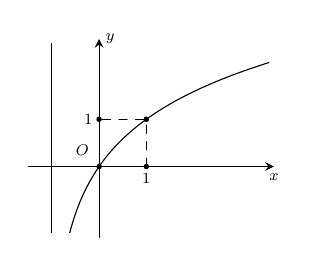
\begin{tikzpicture}[scale=1,font=\footnotesize,line join=round,line cap=round,>=stealth,x=0.6cm,y=0.6cm,declare function = {f (\x) =ln((\x)+1)/ln(2);}]
				\def \xmin{-1.5}; 
				 \def \xmax{3.7};
				\def \ymin{-1.5}; 
				 \def \ymax{2.7};
				\draw[->]  (\xmin,0.) -- (\xmax,0.) node[anchor=north] {$x$};
				\draw[->] (0.,\ymin) -- (0.,\ymax)  node[anchor=west] {$y$};
				 \clip (\xmin+0.1,\ymin+0.1) rectangle (\xmax-0.1,\ymax-0.1);
				\draw[smooth,samples=100,domain=-0.9:\xmax]  plot (\x,{f (\x)});
				\draw  (-1,-1.4)--(-1,3.6);
				\draw[dashed]  (1,0) node[below]{$1$} |- (0,1) node[left]{$1$};
				\foreach \x/\y/\l/\g in {0/0/O/135,1/1//0,1/0//0,0/1//0}{\fill[black] (\x,\y)  circle (1pt)+(\g:0.5) node{$\l$};}
			\end{tikzpicture}
	\end{center}
	\choice 
		{$y=\log_3x$} 
		{$y=\log_2x+1$} 
		{\True $y=\log_2(x+1)$} 
		 {$y=\log_3(x+1)$}
	\loigiai{ 
		Đồ thị hàm số đi qua điểm $(0;0)$ nên loại phương án $y=\log_3x$ và $y=\log_2x+1$.\\ 
		Đồ thị hàm số đi qua  điểm $(1;1)$ nên loại phương án $y=\log_3(x+1)$.\\
		Vậy đáp án $y=\log_2\left(x+1\right)$  thỏa mãn.
	 }
\end{ex}

% nguồn: Ok_TracNghiemLop11_Lan1
\begin{ex}%[1D6H3-3]%[ma:550cae3d]
	Tìm tất cả các giá trị của  $a$ để hàm số $ y = ( 2 - a)^x $ nghịch biến trên $ \mathbb{R} $.
	\choice 
		{$ 2 < a <  3 $}
		{\True $ 1  < a < 2 $}
		{$ a > 2  $}
		{$ 0 < a < 1 $} 
	 \loigiai{
		Hàm số $ y = (2 - a)^x $ nghịch biến trên $  \mathbb{R} \Leftrightarrow 0 < 2 - a < 1 \Leftrightarrow 1 < a < 2 $.
	} 
\end{ex}

% nguồn: Ok_TracNghiemLop11_Lan1
\begin{ex}%[1D6H3-3]%[ma:170cedf8]
	 Mệnh đề nào trong các mệnh đề dưới đây \textbf{sai}?
	 \choice
		{\True Hàm  số $y=\left(\dfrac{2025}{\pi}\right)^{x^2+1}$ đồng biến trên $\mathbb{R}$}
		{Hàm số $y=\log x$ đồng biến trên $(0;+\infty)$} 
		{Hàm số $y=\ln \left(-x\right)$ nghịch biến trên  khoảng $(-\infty;0)$}
		{Hàm  số $y=2^x$ đồng biến trên $\mathbb{R}$}
	\loigiai{ 
		Hàm số $y=\left(\dfrac{2025}{\pi}\right)^{x^2+1}$ có tập xác định $\mathscr{D}=\mathbb{R}$.\\ 
		Ta có $y'=2x\cdot\left(\dfrac{2025}{\pi}\right)^{x^2+1}\cdot  \ln\left(\dfrac{2025}{\pi}\right)$.\\
		Do đó hàm số này không thể đồng biến trên  $\mathbb{R}$.
	 }
\end{ex}

% nguồn: Ok_TracNghiemLop11_Lan1
\begin{ex}%[1D6H3-3]%[ma:892d26d3]
	\immini{ 
	Tìm $a$ để hàm số $y=\log_a x$ $(0<a \ne  1)$ có đồ thị là hình bên.
	\choice 
		 {\True $a=\sqrt{2}$}
		 {$a=\dfrac{1}{\sqrt{2}}$}
		 {$a=\dfrac{1}{2}$}
		{$a=2$} 
		 }{
		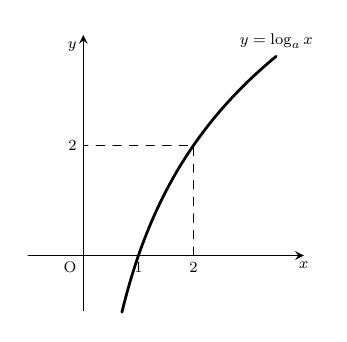
\begin{tikzpicture}[scale=0.7,font=\footnotesize,line join=round,line cap=round,>=stealth]
				\draw[->]  (-1,0)--(0,0) node[below left]{O}--(4,0) node[below]{$x$};
				\draw[->] (0,-1)--(0,4) node[below left]{$y$}; 
				\draw[smooth,black,line width=1,samples=80] plot[domain=0.7:3.5] (\x,{2*log2 (\x)})  node[above]{$y=\log_ax$};
				\draw[dashed] (1,0) node[below]{$1$} 
					 (2,0) node[below]{$2$}
					 (0,2) node[left]{$2$};
				 \draw[dashed] (2,0)--(2,2)--(0,2);
			\end{tikzpicture}
		} 
	\loigiai{Đồ thị hàm số đi qua điểm $(2;2)$ nên $2=\log_a 2 \Leftrightarrow a^2=2  \Leftrightarrow a=\sqrt{2}$.
	} 
\end{ex}

% nguồn: Ok_TracNghiemLop11_Lan1
\begin{ex}%[1D6H3-3]%[ma:00b74eab]
	\immini{ 
	Cho hàm số $y=\log_ax\left(a>0, a\neq 1\right)$ có đồ thị như hình vẽ. Giá trị của $a$  bằng
	\choice 
		 {$a=2$}
		{$a=\sqrt{2}$} 
		 {$a=\dfrac{1}{\sqrt{2}}$}
		{\True  $a=\dfrac{1}{2}$}
		}{ 
		\begin{tikzpicture}[scale=0.7,font=\footnotesize,line join=round,line cap=round,>=stealth]
				\def\xmax{5}  \def\ymin{-3} \def\ymax{3}
				 \draw[->] (-0.9,0)--(\xmax,0) node [below]{$x$};
				\draw[->] (0,\ymin)--(0,\ymax) node [left]{$y$}; 
				\node at (0,0)  [above left]{$O$};
				\clip  (-0.9,\ymin) rectangle (\xmax-0.1,\ymax-0.1);
				\draw[smooth,samples=300,domain=0.03:\xmax] plot  (\x,{ln(\x)/ln(0.5)});
				\draw[dashed]  (2,0) node[above]{$2$}--(2,-1)--(0,-1) node[left]{$-1$};
				\fill (1,0) circle (1.0pt)  node[below]{$1$}
					(2,0) circle  (1.0pt)
					(0,-1) circle  (1.0pt);
			\end{tikzpicture}
		} 
	 \loigiai{
		Đồ thị hàm số $y=\log_ax$ đi qua điểm $(2;-1)$ nên  $\log_a2=-1$.\\
	 Khi đó $a^{-1}=2\Leftrightarrow\dfrac{1}{a}=2\Leftrightarrow a=\dfrac{1}{2}$.}
\end{ex}

% nguồn: Ok_Toan11_TracNghiem_Lan2
\begin{ex}%[1D6V3-3]%[ma:6c39dc52]
	Biết hàm số $f(x)=\dfrac{a}{b^2\cdot 3^x}$ có đồ thị đối xứng với đồ thị hàm số $y=3^x$ qua  đường thẳng $x=-1$. Biết $a$, $b$ là các số nguyên. Chọn khẳng định đúng trong các khẳng định sau:
	\begin{center}
		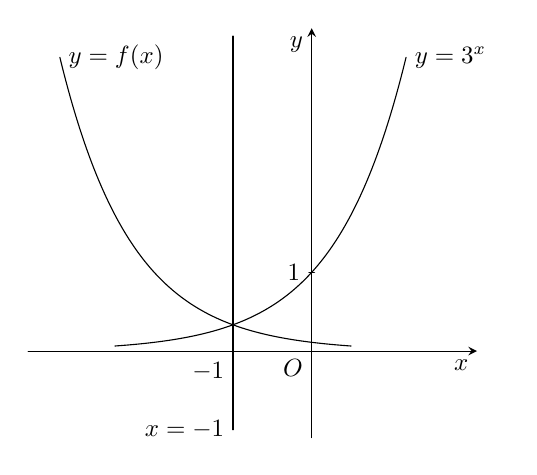
\begin{tikzpicture}[line join=round,line cap=round,>=stealth]
				\tikzset{every  node/.style={scale=0.9}}
				\draw[->] (-3.6,0)--(2.1,0)  node[below left] {$x$};
				\draw[->] (0,-1.1)--(0,4.1) node[below  left] {$y$};
				\draw (0,0)  node [below left] {$O$};
				\foreach \x/\nx in {-1/-1} 
				\draw[thin] (\x,1pt)--(\x,-1pt) node [below left] {$\nx$}; 
				\foreach \y/\ny in {1/1} 
				 \draw[thin] (1pt,\y)--(-1pt,\y) node [left] {$\ny$};
				\begin{scope}
					\clip (-3.5,-1) rectangle  (2.5,4);
					\draw[samples=200,domain=-2.5:1.2,smooth,variable=\x]  plot (\x,{3^(\x)}) node[right]{$y=3^x$};
					 \draw[samples=200,domain=0.5:-3.2,smooth,variable=\x] plot (\x,{1/(3^((\x)+2))}) node[right]{$y=f (x)$};
				\end{scope}
				 \draw (-1,4)--(-1,-1) node[left]{$x=-1$};
			\end{tikzpicture}
	\end{center}
	 \choice
		{\True  $b^2=9a$}
		{$b^2=4a$} 
		{$b^2=6a$} 
		 {$b^2=a$}
	 \loigiai{
		\begin{center}
			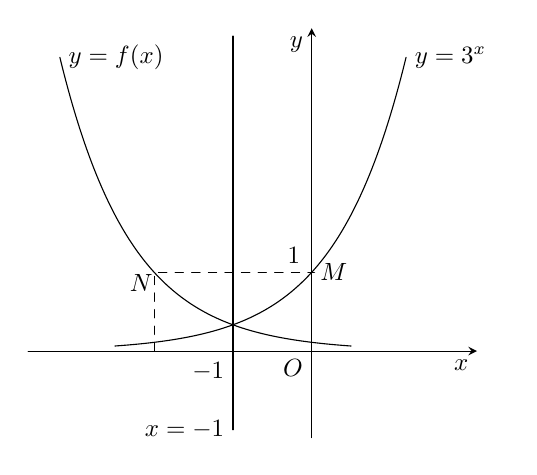
\begin{tikzpicture}[line join=round,line cap=round,>=stealth]
					\tikzset{every node/.style={scale=0.9}} 
					\draw[->] (-3.6,0)--(2.1,0) node[below  left] {$x$};
					\draw[->]  (0,-1.1)--(0,4.1) node[below left] {$y$};
					\draw (0,0) node [below left]  {$O$};
					 \foreach \x/\nx in {-1/-1}
					\draw[thin]  (\x,1pt)--(\x,-1pt) node [below left] {$\nx$};
					\foreach \y/\ny  in {1/1}
					\draw[thin] (1pt,\y)--(-1pt,\y) node [above  left] {$\ny$};
					\begin{scope}
						\clip (-3.5,-1) rectangle (2.5,4); 
						\draw[samples=200,domain=-2.5:1.2,smooth,variable=\x] plot  (\x,{3^(\x)}) node[right]{$y=3^x$};
						\draw[samples=200,domain=0.5:-3.2,smooth,variable=\x] plot  (\x,{1/(3^((\x)+2))}) node[right]{$y=f (x)$};
					\end{scope}
					\draw  (-1,4)--(-1,-1) node[left]{$x=-1$};
					\draw[dashed](-2,0)--(-2,1)--(0,1); 
					\node[right]  at (0,1) {$M$};
					 \node[below left=-0.1cm] at (-2,1) {$N$};
				\end{tikzpicture}
		\end{center}
		Trên đồ thị hàm số $y=3^x$ lấy $M(x_0;y_0)$ và gọi $N\Big(x,f(x)\Big)$ là điểm thuộc đồ thị hàm số $f(x)$ và đối xứng với $M$ qua đường thẳng  $x=-1$.\\
		 Khi đó $\heva{&\dfrac{x+x_0}{2}=-1\\&f(x)=y_0}\Leftrightarrow \heva{&x_0=-x-2\\&y_0=f(x).}$\\
		 Thay vào hàm số $y=3^x$ ta được $f(x)=3^{-x-2}=\dfrac{1}{3^23^x}$.\\
		Vậy $a=1$;  $b=3\Rightarrow b^2=9a$.
	} 
\end{ex}

% nguồn: Ok_Toan11_TracNghiem_Lan2
\begin{ex}%[1D6V3-3]%[ma:77249fd0]
	Cho $a$, $b$ là các số thực dương khác $1$, đường thẳng $d$ song song trục hoành cắt trục tung, đồ thị hàm số $y=a^x$, đồ thị hàm số $y=b^x$ lần lượt tại $H$, $M$, $N$ (như hình  bên). Biết $HM=3MN$. Mệnh đề nào sau đây đúng?
	\begin{center}
		\begin{tikzpicture}[line join=round,line cap=round,>=stealth]
				\tikzset{every  node/.style={scale=0.9}}
				\draw[->] (-1.1,0)--(4.1,0)  node[below left] {$x$};
				\draw[->] (0,-1.1)--(0,4.1)  node[below left] {$y$};
				\draw (0,0) node  [below left] {$O$};
				\foreach \y/\ny in  {1/1}
				\draw[thin]  (1pt,\y)--(-1pt,\y) node [above left] {$\ny$};
				\begin{scope}
					\clip (-1,-1.5) rectangle (5,4.1); 
					\draw[samples=200,domain=-1:1.5,smooth,variable=\x] plot (\x,{2.5^(\x)})  node[right]{$y=a^x$};
					\draw[samples=200,domain=-1:3.3,smooth,variable=\x] plot  (\x,{1.5^(\x)}) node[right]{$y=b^x$};
				\end{scope}
				 \coordinate (O) at (0,0);
				 \coordinate (H) at (0,3);
				 \coordinate (h) at (4,3);
				\path[name path=ax,samples=200,domain=-1:1.5,smooth,variable=\x] plot  (\x,{2.5^(\x)});
				\path[name path=bx,samples=200,domain=-1:3.3,smooth,variable=\x]  plot (\x,{1.5^(\x)});
				\path [name path=Hh]  (H)--(h);
				 \path [name intersections={of=ax and Hh,by={M}}];
				\path [name intersections={of=bx and Hh,by={N}}]; 
				\coordinate (Mx) at  (M|-O);
				\coordinate (Nx) at  (N|-O);
				\draw[dashed] (H)--(N) 
					 (M)--(Mx)
					(N)--(Nx); 
				 \foreach \i/\g in {H/180,M/135,N/135}{\draw[fill=white](\i)
					($(\i)+(\g:3mm)$)  node[scale=1]{$\i$};}
			\end{tikzpicture}
	\end{center}
	\choice 
		{$4a=3b$} 
		{\True $b^4=a^3$} 
		{$b^3=a^4$} 
		{$3a=4b$} 
	\loigiai{ 
		Đường thẳng $d$ cắt đồ thị hàm số  $y=a^x$ tại điểm $M\left(x_M;y_M\right) \Rightarrow y_M=a^{x_M}$.\\
		Đường thẳng  $d$ cắt đồ thị hàm số $y=b^x$ tại điểm $N\left(x_N;y_N\right) \Rightarrow y_N=b^{x_N}$.\\
		Mà $y_M=y_N$  $\Rightarrow a^{x_M}=b^{x_N}$.\\
		Ta có $HM=3MN$ hay $HM=\dfrac{3}{4}HN$.\\ 
		Khi đó $x_M=\dfrac{3}{4}{x_N}\Rightarrow a^{\tfrac{3}{4} x_N}=b^{x_N}\Leftrightarrow a^{\tfrac{3}{4}}=b \Leftrightarrow  a^3=b^4$.
	 }
\end{ex}

% nguồn: Ok_Toan11_TracNghiem_Lan2
\begin{ex}%[1D6V3-3]%[ma:cc26020c]
	Đồ thị hàm số $y=f(x)$ đối xứng  với đồ thị hàm số $y=a^x$ với $a>0$, $a\ne 1$ qua điểm $I(1;1)$. Giá trị của biểu thức $f\left(2+\log_a\dfrac{1}{2\,023}\right)$ bằng
	 \choice
		 {$2\,022$}
		 {$2\,024$}
		{$-2\,023$} 
		{\True $-2\,021$} 
	 \loigiai{
		 Gọi $(C)$ là đồ thị hàm số $y=a^x$; $(C_1)$ là đồ thị hàm số $y=f(x)$.\\
		Khi đó $M\left(2+\log_a\dfrac{1}{2\,023};y_M\right)\in (C_1)$.\\ 
		Suy ra  $y_M=f\left(2+\log_a\dfrac{1}{2\,023}\right)$.\\
		Gọi $N$ đối xứng với $M$ qua $I(1;1)$.\\ 
		Suy  ra $N\left(-\log_a\dfrac{1}{2\,023};2-y_M\right)$.\\
		 Do đồ thị $(C_1)$ đối xứng $(C)$ qua $I(1;1)$ nên $N\left(-\log_a\dfrac{1}{2\,023};2-y_M\right)\in(C)$.\\
		 Suy ra
		\allowdisplaybreaks 
		\begin{eqnarray*}
			2-y_M=a^{-\log_a\dfrac{1}{2\,023}}&\Leftrightarrow&2-y_M=a^{\log_a2\,023}\\ 
			 &\Leftrightarrow&2-y_M=2\,023\\
			 &\Leftrightarrow&y_M=-2\,021.
		\end{eqnarray*}
		Vậy $f\left(2+\log_a\dfrac{1}{2\,023}\right)=-2\,021$. 
	 }
\end{ex}

% nguồn: Ok_Toan11_TracNghiem_Lan2
\begin{ex}%[1D6V3-3]%[ma:6237e64a]
	Đồ thị hàm số $y=f(x)$ đối xứng với  đồ thị của hàm số $y=2\,022^x$ qua điểm $I(1;1)$. Giá trị của biểu thức $f\left(2+\log_{2\,022}\dfrac{1}{2\,023}\right)$ bằng
	\choice 
		{\True  $-2\,021$}
		{$-2\,023$} 
		 {$-2\,020$}
		 {$2\,020$}
	\loigiai{ 
		\begin{center}
			\begin{tikzpicture}[line join=round,line cap=round,>=stealth,scale=0.8]
					\tikzset{every node/.style={scale=0.9}} 
					\begin{scope}
						 \clip (-3,-3) rectangle (5,5);
						\draw[samples=200,domain=-3:0.2,smooth,variable=\x] plot (\x,{2022^(\x)}) node[right]{$y=2\,022^x$}; 
						\draw[samples=200,domain=1.8:5,smooth,variable=\x] plot (\x,{2-2022^(2-(\x))}) node[above left]{$y=f (x)$}; 
					\end{scope}
					 \draw (1,1) circle (1.0pt) node[below]{$I (1,1)$};
					\draw (2,1) circle (1.0pt)  node[right]{$M$};
					\draw  (0,1) circle (1.0pt) node[left]{$N$};
					\draw  (0,1)--(2,1);
				\end{tikzpicture}
		\end{center}
		Gọi $N\in(C)\colon y=f(x)\Rightarrow N\left(x;f(x)\right)$, $M$  là điểm đối xứng với $N$ qua $I$.\\
		Suy ra $M\in(S)\colon y=2\,022^x$ và $I(1;1)$ là trung điểm $MN$.\\ 
		Suy ra $M\left(2-x;2-f(x)\right)$.\\ 
		Mà $M\in(S)\Rightarrow 2-f(x)=2\,022^{2-x}\Rightarrow  f(x)=2-2\,022^{2-x}$.\\
		Khi đó ta có 
		\allowdisplaybreaks 
		\begin{eqnarray*}
			 f\left(2+\log_{2\,022}\dfrac{1}{2\,023}\right)&=&2-2\,022^{2-\left(2+\log_{2\,022}\dfrac{1}{2\,023}\right)}\\
			 &=&2-2\,022^{\log_{2\,022}2\,023}\\
			&=&2-2\,023=-2\,021. 
		\end{eqnarray*}
	} 
\end{ex}

% nguồn: Ok_TracNghiemLop11_Lan1
\begin{ex}%[1D6V3-3]%[ma:c65a8dc1]
	\immini{Cho đồ thị hàm số $y=a^x$ và $y=\log_bx$ như  hình vẽ bên. Khẳng định nào sau đây đúng?
	\choice 
		{$0<a<\dfrac{1}{2}<b$} 
		{\True $0<a<1<b$} 
		{$0<b<1<a$} 
		{$0<a<1$, $0<b<\dfrac{1}{2}$}}{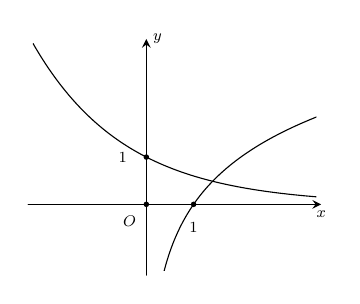
\begin{tikzpicture}[scale=1,font=\footnotesize,line join=round,line cap=round,>=stealth,x=0.6cm,y=0.6cm,declare function = {f (\x)=ln(\x)/ln(2); g (\x)=0.6^(\x);}]
		\def  \xmin{-2.5};
		\def  \xmax{3.7};
		 \def \ymin{-1.5};
		 \def \ymax{3.5};
		\draw[->] (\xmin,0.) -- (\xmax,0.) node[anchor=north] {$x$}; 
		\draw[->] (0.,\ymin) --  (0.,\ymax) node[anchor=west] {$y$};
		\clip (\xmin+0.1,\ymin+0.1) rectangle (\xmax-0.1,\ymax-0.1); 
		 \draw[smooth,samples=100,domain=0.1:\xmax] plot (\x,{f (\x)});
		\draw[smooth,samples=100,domain=\xmin:\xmax] plot (\x,{g (\x)}); 
		\foreach \x/\y/\l/\g in {0/0/O/225,0/1/1/180,1/0/1/-90}{\fill[black] (\x,\y) circle (1pt)+(\g:0.5)  node{$\l$};}
	\end{tikzpicture}
		 }
	\loigiai{ 
		Đồ thị hàm số $y=a^x$ đi qua $\left(0;1\right)$ nên từ hình vẽ suy ra hàm số $y=a^x$ là hàm  nghịch biến. Do đó $0<a<1$.\\
		Đồ thị hàm số $y=\log_bx$ đi qua $\left(1;0\right)$ nên từ hình vẽ suy ra hàm số  $y=\log_b x$ là hàm đồng biến. Do đó $b>1$.\\
		 Vậy $0<a<1<b$.
	 }
\end{ex}

% nguồn: Ok_TracNghiemLop11_Lan1
\begin{ex}%[1D6V3-3]%[ma:165cd4b7]
	 Biết đồ thị của hàm số $y=f\left(x\right)$ đối xứng với đồ thị hàm số $y=\log_ax \, \left(0<a\ne 1\right)$ qua điểm $I\left(2;2\right)$. Giá trị của $f\left(4-a^{2018}\right)$ là
	\choice 
		 {$-2020$}
		{$2014$} 
		 {\True $-2014$}
		 {$2020$}
	 \loigiai{
	Gọi $M\left(x;\log_ax\right)$ là điểm thuộc đồ thị  hàm số $y=\log_ax$ thì điểm đối xứng với $M$ qua $I$ là ${M}'\left(4-x;4-\log_ax\right)$ thuộc đồ thị hàm số $y=f(x)$.\\
	Do đó $f\left(4-x\right)=4-\log_ax$. 
	Suy ra: $f\left(4-a^{2018}\right)=4-\log_aa^{2018}=-2014$ 
	 }
\end{ex}

% nguồn: Ok_TracNghiemLop11_Lan1
\begin{ex}%[1D6V3-3]%[ma:08b22a58]
	 \immini
	{ 
	 Cho hai hàm số $y=\log_a x$ và $y=\log_b x$ có đồ thị như hình vẽ. Mệnh đề nào sau đây là đúng?
	 \choice
		 { $a>b>1$}
		{$1>a>b$} 
		{\True$b>a>1$} 
		{$a>1>b$} 
		}{ 
		\begin{tikzpicture}[>=stealth,scale=0.8,line join=round,line cap=round]
				 \draw[->] (-1,0)--(6,0) node [below]{$x$};
				\draw[->] (0,-1)--(0,3)  node [left]{$y$};
				 \node at (0,0) [below left]{$O$};
				 \clip (-1,-1) rectangle (5,4);
				 \fill[black] (1,0) circle (1pt) node [below] {$1$};
				\draw[smooth,samples=150,domain=0.1:5] plot (\x,{ln(\x)/ln(3)}); 
				\draw[smooth,samples=150,domain=0.1:5]  plot (\x,{ln(\x)/ln(2)});
				 \node at (2.5,0.6)[right]{$y=\log_b x$};
				\node at  (1,1.9)[right]{$y=\log_a x$};
			\end{tikzpicture}
		} 
	 \loigiai{
	\immini{ 
		Quan sát đồ thị ta thấy cả  hai đồ thị đều đi lên từ trái sang phải nên $a>1$ và $b>1$.\\
		Kẻ đường thẳng $y=1$ lần  lượt cắt hai đồ thị $y=\log_a x$ và $y=\log_b x$ tại hai điểm $A(a;1); B(b;1)$. \\Nhìn vào đồ thị ta thấy $a< b$.
		 }{
		\begin{tikzpicture}[>=stealth,scale=0.8,line join=round,line cap=round]
				\draw[->] (-1,0)--(5,0)  node [below]{$x$};
				\draw[->] (0,-1)--(0,3) node [left]{$y$}; 
				\node at (0,0) [below  left]{$O$};
				\clip (-1,-1) rectangle  (5,4);
				\draw  (-1,1)--(5,1);
				\fill[black] (1,0) circle  (1pt) node [below] {$1$};
				\fill [black] (2,1) circle (1pt)  node [above] {$A$};
				\fill [black] (3,1) circle (1pt) node [above]  {$B$};
				\draw  [dashed] (2,1)--(2,0) node [below] {$a$};
				\draw [dashed] (3,1)--(3,0) node  [below] {$b$};
				 \node at (0,1) [below left]{$1$};
				\draw[smooth,samples=150,domain=0.1:5]  plot (\x,{ln(\x)/ln(3)});
				\draw[smooth,samples=150,domain=0.1:5] plot (\x,{ln(\x)/ln(2)}); 
				\node at  (2.5,0.6)[right]{$y=\log_bx$};
				\node at (1,1.9)[right]{$y=\log_ax$}; 
			\end{tikzpicture}
		 }
	} 
\end{ex}

% nguồn: Ok_TracNghiemLop11_Lan1
\begin{ex}%[1D6V3-3]%[ma:70a3ed3e]
	\immini{ Cho $a,\,b,\,c$ là  các số thực dương và khác $1$. Hình vẽ dưới đây là đồ thị của hàm số $y=\log_ax,\,y=\log_bx,\,y=\log_cx$. Khẳng định nào sau đây là đúng?
	 \choice
		{$c<a<b$} 
		 {\True $b<c<a$}
		{$b<a<c$} 
		{$a<b<c$}} 
		{\begin{tikzpicture}[scale=0.7,font=\footnotesize,line join=round,line cap=round,>=stealth]
		\draw[->] (-1.1,0)--(6.1,0)  node[below left] {$x$};
		\draw[->]  (0,-3)--(0,3) node[below left] {$y$};
		\draw (0,0)  node [below left] {$O$};
		\begin{scope}
			 \clip (-1,-4) rectangle (5,4);
			\draw[samples=200,domain=0.17:4,smooth,variable=\x]  plot (\x,{ln((\x))/ln(3)});
			\draw[samples=200,domain=0.17:4,smooth,variable=\x]  plot (\x,{ln((\x))/ln(2)});
			\draw[samples=200,domain=0.17:4,smooth,variable=\x]  plot (\x,{ln((\x))/ln(0.5)});
		\end{scope}
		\draw (3.9,-2) node[right]{$y={\log_{b}}x$}; 
		\draw  (3.9,2) node[right]{$y={\log_{c}}x$};
		\draw  (3.9,1) node[right]{$y={\log_{a}}x$};
		\draw (1,0)  node[below]{$1$};
	\end{tikzpicture}
		 }
	\loigiai{\immini{ 
		Ta vẽ thêm đường thẳng $y=1$ vào đồ  thị đã cho.\\
		Nhận thấy rằng đường thẳng $y=1$ cắt 3 đồ thị $y=\log_ax,\,y=\log_bx,\,y=\log_cx$ lần lượt với $3$ giao  điểm có hoành độ $x=a,\,x=b,\,x=c$.\\
		Dựa vào hình vẽ ta  thấy $b<c<a$. }{
		\begin{tikzpicture}[scale=0.9,font=\footnotesize,line join=round,line cap=round,>=stealth]
				\draw[->] (-1.1,0)--(5,0)  node[below left] {$x$};
				\draw[->] (0,-3)--(0,3.2)  node[below left] {$y$};
				\draw (0,0) node  [below left] {$O$};
				\draw[dashed](3,0)--(3,1)--(0,1); 
				\draw[dashed](2,0)--(2,1)--(0,1); 
				 \draw[dashed](0.5,0)--(0.5,1)--(0,1);
				\begin{scope}
					\clip  (-1,-4) rectangle (5,4);
					\draw[samples=200,domain=0.17:4,smooth,variable=\x] plot (\x,{ln((\x))/ln(3)}); 
					\draw[samples=200,domain=0.17:4,smooth,variable=\x] plot  (\x,{ln((\x))/ln(2)});
					 \draw[samples=200,domain=0.17:4,smooth,variable=\x] plot (\x,{ln((\x))/ln(0.5)});
					\draw  (1.95,-2) node[right]{$y={\log_{b}}x$};
					\draw (2.2,2.3)  node[right]{$y={\log_{c}}x$};
					 \draw (3.1,0.95) node[right]{$y={\log_{a}}x$};
					\draw  (0,1) node[left]{$1$};
					\draw (1,0)  node[below]{$1$};
					\draw (2,0)  node[below]{$c$};
					\draw  (3,0) node[below]{$a$};
					 \draw (0.5,0) node[below]{$b$};
				\end{scope}
			\end{tikzpicture}
		 }
	 }
\end{ex}

% nguồn: Ok_TracNghiemLop11_Lan1
\begin{ex}%[1D6V3-3]%[ma:90ccd2b1]
	\immini 
	 {
	Trong hình vẽ bên các đồ thi hàm số $y=\log_ax$, $y=\log_bx$, $y=\log_cx$ với $(0<a, b, c\ne 1)$ cắt các đường thẳng $x=4$, $x=8$ tạo thành hình vuông $MNPQ$ có cạnh bằng $4$. Biết rằng $abc=2^{\tfrac{x}{y}}$ với $x$, $y\in\mathbb{R}^+$ và  $\dfrac{x}{y}$ tối giản, giá trị của $y-x$ bằng
	 \choice
		{$34$} 
		{\True  $5$}
		 {$19$}
		{$43$} 
		 }
		{ 
		\begin{tikzpicture}[line join=round,line cap=round,>=stealth,scale=0.5]
				\tikzset{every node/.style={scale=0.9}} 
				\draw[->] (-1.1,0)--(10.1,0) node[below left] {$x$}; 
				\draw[->]  (0,-1.1)--(0,14.1) node[below left] {$y$};
				\draw  (0,0) node [below left] {$O$};
				 \foreach \x/\nx in {4/4,8/8}
				\draw[thin]  (\x,1pt)--(\x,-1pt) node [below] {$\nx$};
				\begin{scope}
					\clip (-1,-1) rectangle  (10,14);
					 \draw[samples=200,domain=0.5:9,smooth,variable=\x] plot (\x,{ln((\x))/ln(2^(0.25))}) node[above,sloped]{$\log_bx$};
					\draw[samples=200,domain=0.5:9,smooth,variable=\x] plot (\x,{ln((\x))/ln(2^(0.375))}) node[sloped,above]{$\log_ax$}; 
					 \draw[samples=200,domain=0.5:4.5,smooth,variable=\x] plot (\x,{ln((\x))/ln(2^(0.166667))}) node[above,sloped]{$\log_cx$};
				\end{scope}
				\draw  (-1,8)--(0,8) node[above left]{$m$}--(4,8) node[below right]{$M$}--(8,8) node[below right]{$N$}--(10,8)
					(-1,12)--(0,12) node[above left]{$m+4$}--(4,12) node[below right]{$Q$}--(8,12) node[below  right]{$P$}--(10,12);
				 \draw[dashed]
					 (4,0)--(4,12)
					 (8,0)--(8,12);
			\end{tikzpicture}
		 }
	 \loigiai{
		Hình vuông $MNPQ$ có tọa độ các đỉnh là $M\left(4;\log_b4\right)$, $N\left(8;\log_a8\right)$, $P\left(8;\log_b8\right)$ và  $Q\left(4;\log_c4\right)$.\\
		Ta có $\heva{&\log_c4=\log_b8\\&\log_c4-\log_b4=4}\Rightarrow \log_b8-\log_b4=4\Leftrightarrow \log_b2=4\Leftrightarrow b^4=2\Leftrightarrow b=2^{\tfrac{1}{4}}$.\\ 
		Do $\log_b4=\log_a8$ nên $\log_{2^{\tfrac{1}{4}}}2^2=\log_a8\Leftrightarrow \log_a8=8\Leftrightarrow  a^8=8\Leftrightarrow a=\sqrt[8]{8}=2^{\tfrac{3}{8}}$.\\
		Mà $\log_c4=\log_b8$ nên $\log_c4=\log_{2^{\tfrac{1}{4}}}2^3\Leftrightarrow \log_c4=12\Leftrightarrow c^{12}=4\Leftrightarrow  c=\sqrt[12]{4}=2^{\tfrac{1}{6}}$.\\
		Khi đó  $abc=2^{\tfrac{3}{8}}\cdot 2^{\tfrac{1}{4}}\cdot 2^{\tfrac{1}{6}}=2^{\tfrac{19}{24}}$.\\
		Vậy $x=19$ và $y=24$  nên $y-x=24-19=5$.
	 }
\end{ex}

% nguồn: Ok_TracNghiemLop11_Lan1
\begin{ex}%[1D6V3-3]%[ma:2558c99b]
	\immini 
	 {
	Cho ba hàm số $y=a^x,y=b^x, y=c^x$, với $a,b,c$ là hai số thực dương khác $1$ lần  lượt có đồ thị như hình bên. Khẳng định nào sau đây đúng?
	\choice 
		{$a<b<c$} 
		{\True  $a<c<b$}
		 {$b<c<a$}
		 {$c<a<b$}
		}{ 
		\begin{tikzpicture}[scale=1,font=\footnotesize,line join=round,line cap=round,>=stealth]
				\def\xmin{-4}\def\xmax{5}\def\ymin{-1}\def\ymax{4} 
				 \draw[->] (\xmin-0.2,0)--(\xmax+0.2,0) node[below] {\footnotesize $x$};
				\draw[->]  (0,\ymin-0.2)--(0,\ymax+0.2) node[right] {\footnotesize $y$};
				\draw (0,0) node [below left]  {\footnotesize $O$};
				\foreach \x in {}\draw (\x,0.1)--(\x,-0.1) node [below] {\footnotesize  $\x$};
				\foreach \y in {1}\draw (0.1,\y)--(-0.1,\y) node [left] {\footnotesize  $\y$};
				\clip  (\xmin,\ymin) rectangle (\xmax,\ymax);
				 \draw[smooth,samples=200,domain=\xmin:\xmax] plot (\x,{3^\x});
				 \draw (1.2,3.8) node [right]{$y=b^x$};
				 \draw[smooth,samples=200,domain=\xmin:\xmax] plot (\x,{.5^\x});
				 \draw (-1.9,3.8) node [right]{$y=a^x$};
				 \draw[smooth,samples=200,domain=\xmin:\xmax] plot (\x,{1.7^\x});
				\draw (2,3) node  [right]{$y=c^x$};
			\end{tikzpicture}
		} 
	\loigiai{\immini{ Kẻ đường thẳng $x=1$ cắt các đồ thị hàm số  tại các điểm lần lượt có tung độ là $a,c,b$ như hình trên.
	Từ  đồ thị ta có
	\[ 
	 0<a<1<c<b.
	 \]
	 }
	{ 
	\begin{tikzpicture}[scale=1,font=\footnotesize,line join=round,line cap=round,>=stealth]
			 \def\xmin{-4}\def\xmax{5}\def\ymin{-1}\def\ymax{4}
			\draw[->] (\xmin-0.2,0)--(\xmax+0.2,0) node[below]  {\footnotesize $x$};
			\draw[->] (0,\ymin-0.2)--(0,\ymax+0.2) node[right] {\footnotesize $y$}; 
			\draw (0,0)  node [below left] {\footnotesize $O$};
			\foreach \x in {}\draw (\x,0.1)--(\x,-0.1) node [below] {\footnotesize $\x$}; 
			\foreach \y in {1}\draw (0.1,\y)--(-0.1,\y)  node [left] {\footnotesize $\y$};
			\clip (\xmin,\ymin) rectangle  (\xmax,\ymax);
			\draw[smooth,samples=200,domain=\xmin:\xmax]  plot (\x,{3^\x});
			 \draw (1.2,3.8) node [right]{$y=b^x$};
			\draw[smooth,samples=200,domain=\xmin:\xmax] plot  (\x,{.5^\x});
			\draw (-1.9,3.8) node [right]{$y=a^x$}; 
			 \draw[smooth,samples=200,domain=\xmin:\xmax] plot (\x,{1.7^\x});
			\draw (2,3) node  [right]{$y=c^x$};
			\draw[dashed] (1,-1.3)  node[below]{$1$}--(1,4.1)
				(1,3)--(0,3)  node[left]{$b$}
				(1,.5)--(0,.5)  node[left]{$a$}
				(1,1.7)--(0,1.7) node[left]{$c$}; 
		\end{tikzpicture}
	 }
	 }
\end{ex}

% nguồn: Ok_TracNghiemLop11_Lan1
\begin{ex}%[1D6V3-3]%[ma:8123265b]
	\immini{ 
	Cho các hàm số $y=\log_ax$; $y=\log_bx$; $y=\log_cx$ có đồ thị như hình vẽ. Khẳng định nào sau đây  đúng?
	\choice 
		{\True  $a>c>b$}
		 {$a>b>c$}
		{$c>a>b$} 
		{$b>c>a$} 
		 }{
		\begin{tikzpicture}[scale=0.7,font=\footnotesize,line join=round,line cap=round,>=stealth]
				\def\xmax{5} \def\ymin{-3} \def\ymax{3} 
				\draw[->] (-0.9,0)--(\xmax,0) node [below]{$x$}; 
				\draw[->] (0,\ymin)--(0,\ymax)  node [left]{$y$};
				\node at (0,0)  [above left]{$O$};
				 \node at (5,-2.2) [right]{$y=\log_ax$};
				 \node at (5,1.5) [right]{$y=\log_bx$};
				\node at  (5,2.5) [right]{$y=\log_cx$};
				\clip (-0.9,\ymin) rectangle  (\xmax-0.1,\ymax-0.1);
				\draw[smooth,samples=300,domain=0.03:\xmax]  plot (\x,{ln(\x)/ln(0.5)})
					plot (\x,{ln(\x)/ln(2)}) plot  (\x,{ln(\x)/ln(3)});
				 \fill (1,0) circle (1.0pt) node[below]{$1$}
					(2,0) circle  (1.0pt)
					(0,-1)  circle (1.0pt);
			\end{tikzpicture}
		} 
	 \loigiai{
		Dựa vào đồ thị ta có hàm số $y=\log_bx$ là một hàm số nghịch biến trên tập xác định của nó nên $0<b<1$; hàm số  $y=\log_ax$; $y=\log_cx$ là các hàm số đồng biến trên tập xác định của nó nên $a>1$ và $c>1$.
		\begin{center}
			\begin{tikzpicture}[scale=0.7,font=\footnotesize,line join=round,line cap=round,>=stealth]
					 \def\xmax{5} \def\ymin{-3} \def\ymax{3}
					\draw[->]  (-0.9,0)--(\xmax,0) node [below]{$x$};
					\draw[->] (0,\ymin)--(0,\ymax) node  [left]{$y$};
					 \node at (0,0) [below left]{$O$};
					\node  at (5,-2.2) [right]{$y=\log_ax$};
					\node at (5,1.5)  [right]{$y=\log_bx$};
					\node  at (5,2.5) [right]{$y=\log_cx$};
					\draw (-1,1)--(5,1) node[right]{$y=1$}; 
					 \clip (-0.9,\ymin) rectangle (\xmax-0.1,\ymax-0.1);
					\draw[smooth,samples=300,domain=0.03:\xmax]  plot (\x,{ln(\x)/ln(0.5)})
						plot (\x,{ln(\x)/ln(2)}) plot  (\x,{ln(\x)/ln(3)});
					\fill (1,0) circle (1.0pt) node[below]{$1$} 
						 (2,0) circle (1.0pt)
						(0,-1) circle  (1.0pt);
				\end{tikzpicture}
		\end{center}
		Kẻ đường thẳng  $y=1$ cắt đồ thị các hàm số $y=\log_cx$; $y=\log_ax$ lần lượt tại các điểm $A(c; 1)$ và $B(a; 1)$.\\
		Dựa vào đồ thị  ta thấy $x_A<x_B\Leftrightarrow c<a$.\\
	 Vậy $a>c>b$.}
\end{ex}

% nguồn: Ok_TracNghiemLop11_Lan1
\begin{ex}%[1D6V3-3]%[ma:72e32243]
	\immini{Cho ba số thực  dương $a$, $b$, $c$ khác $1$. Đồ thị các hàm số $y=a^x$, $y=b^x$, $y=c^x$ được cho trong hình vẽ bên. Mệnh đề nào dưới đây đúng?
	 \choice
		{$b<c<a$} 
		 {$c<a<b$}
		 {$a<b<c$}
		{\True $a<c<b$}}{\begin{tikzpicture}[scale=1,font=\footnotesize,line join=round,line cap=round,>=stealth,x=0.6cm,y=0.6cm,declare function={f (\x)=2^(\x); g (\x)=3^(\x); h (\x)=0.5^(\x);}]
		\def \xmin{-3.0}; 
		\def \xmax{3.5}; 
		\def \ymin{-1.0}; 
		\def  \ymax{5.5};
		 \draw[->] (\xmin,0.) -- (\xmax,0.) node[anchor=north] {$x$};
		\draw[->] (0.,\ymin) -- (0.,\ymax) node[anchor=west]  {$y$};
		\clip  (\xmin+0.1,\ymin+0.1) rectangle (\xmax-0.1,\ymax-0.1);
		\draw[smooth,samples=100,domain=\xmin:\xmax]  plot (\x,{f (\x)}) plot (\x,{g (\x)}) plot (\x,{h (\x)});
		\draw (-2,\ymax) node[right,rotate=-70]{$y=a^x$} 
			 (1.2,\ymax) node[left,rotate=80]{$y=b^x$}
			(2.3,\ymax-2) node[right,rotate=70]{$y=c^x$}; 
		\foreach  \x/\y/\l/\g in {0/0/O/225,0/1/1/180}{\fill[black] (\x,\y) circle (1pt)+(\g:0.5) node{$\l$};}
	\end{tikzpicture}
		 }
	\loigiai{ 
	\immini{Đường thẳng $x=1$ cắt đồ thị các  hàm số $y=a^x,y=b^x,y=c^x$ tại các điểm có tung độ lần lượt là $y=a$, $y=b$, $y=c$ như hình vẽ bên.\\
		Từ đồ thị kết luận $a<c<b$.}{\begin{tikzpicture}[scale=1,font=\footnotesize,line join=round,line cap=round,>=stealth,x=0.6cm,y=0.6cm,declare function={f (\x)=2^(\x); g (\x)=3^(\x); h (\x)=0.5^(\x);}]
		\def \xmin{-3.0}; 
		\def \xmax{3.5}; 
		\def  \ymin{-1.0};
		 \def \ymax{5.5};
		 \draw[->] (\xmin,0.) -- (\xmax,0.) node[anchor=north] {$x$};
		\draw[->] (0.,\ymin) -- (0.,\ymax) node[anchor=west]  {$y$};
		\clip (\xmin+0.1,\ymin+0.1) rectangle  (\xmax-0.1,\ymax-0.1);
		\draw[smooth,samples=100,domain=\xmin:\xmax]  plot (\x,{f (\x)}) plot (\x,{g (\x)}) plot (\x,{h (\x)});
		 \draw (-2,\ymax) node[right,rotate=-70]{$y=a^x$}
			 (1.2,\ymax) node[left,rotate=80]{$y=b^x$}
			(2.3,\ymax-2)  node[right,rotate=70]{$y=c^x$};
		\draw[dashed](1,0) node[below]{$1$}|-(0,3)  node[left]{$b$}
			 (1,2)--(0,2) node[left]{$c$}
			(1,0.5)--(0,0.5)  node[left]{$a$};
		\foreach \x/\y/\l/\g in {0/0/O/225,0/1/1/180,1/0.5//0,1/2//0,1/3//0,1/0//0,0/0.5//0,0/2//0,0/3//0}{\fill[black] (\x,\y) circle  (1pt)+(\g:0.5) node{$\l$};}
	\end{tikzpicture}
		} 
	 }
\end{ex}

% nguồn: Ok_TracNghiemLop11_Lan1
\begin{ex}%[1D6V3-3]%[ma:e26eb24f]
	\immini{Cho đồ thị hàm số $y=a^x$ và $y=\log_bx$ như hình vẽ bên. Trong các  khẳng định sau, đâu là khẳng định đúng?
	 \choice
		{$0<a<1,0<b<1$} 
		 {$a>1,b>1$}
		{\True  $0<b<1<a$}
		{$0<a<1<b$}}{\begin{tikzpicture}[scale=1,font=\footnotesize,line join=round,line cap=round,>=stealth,x=0.6cm,y=0.6cm,declare function = {f (\x)=ln(\x)/ln(0.5); g (\x)=1.8^(\x);}]
		 \def \xmin{-2.5};
		\def \xmax{3.7}; 
		\def \ymin{-1.5}; 
		 \def \ymax{3.5};
		\draw[->] (\xmin,0.) -- (\xmax,0.)  node[anchor=north] {$x$};
		\draw[->]  (0.,\ymin) -- (0.,\ymax) node[anchor=west] {$y$};
		\clip (\xmin+0.1,\ymin+0.1)  rectangle (\xmax-0.1,\ymax-0.1);
		\draw[smooth,samples=100,domain=0.1:\xmax] plot (\x,{f (\x)}); 
		\draw[smooth,samples=100,domain=\xmin:\xmax]  plot (\x,{g (\x)});
		 \foreach \x/\y/\l/\g in {0/0/O/225,0/1/1/180,1/0/1/-90}{\fill[black] (\x,\y) circle (1pt)+(\g:0.5) node{$\l$};}
	\end{tikzpicture}
		 }
	\loigiai{ 
		Đồ thị hàm số $y=a^x$ đi qua $\left(0;1\right)$ nên  từ hình vẽ suy ra hàm số $y=a^x$ là hàm đồng biến. Do đó $a>1$.\\
		Đồ  thị hàm số $y=\log_bx$ đi qua $\left(1;0\right)$ nên từ hình vẽ suy ra hàm số $y=\log_b x$ là hàm nghịch biến. Do đó $0<b<1$.\\
		Vậy $0<b<1<a$. 
	 }
\end{ex}

% nguồn: Ok_TracNghiemLop11_Lan1
\begin{ex}%[1D6K3-3]%[ma:06017f90]
	Cho hai hàm số $y=2^x$, $y=\log_2x$ có đồ thị như hình  vẽ. Đường thẳng $\Delta $ cắt trục $Oy$, đồ thị hàm số $y=2^x$, đồ thị hàm số $y=\log_2x$ và trục $Ox$ lần lượt tại $A$, $B$, $C$, $D$ thỏa mãn $AB=BC=CD$. Hỏi có bao nhiêu đường thẳng $\Delta $ như thế?
	\begin{center}
		\begin{tikzpicture}[scale=1,>=stealth,font=\footnotesize,line join=round,line cap=roundm,x=0.6cm,y=0.6cm]
				\def  \xmin{-3};
				\def  \xmax{6.5};
				\def  \ymin{-2.5};
				\def  \ymax{4.5};
				\draw[->]  (\xmin,0) -- (\xmax,0) node[above] {$x$};
				 \draw[->] (0.,\ymin) -- (0.,\ymax) node[right] {$y$};
				 \draw[smooth,samples=100,domain=-1:2] plot (\x,{(2^(\x))}) node[right]{$y=b^x$};
				 \draw[smooth,samples=100,domain=0.3:5.4] plot (\x,{(ln(\x))/(ln(2))}) node[above]{$y=\log_ax$};
				 \draw (-1,4)--(4,-1);
				\foreach \x/\y/\l/\g in {0/0/O/135,0/1//0,0/1/1/180,1/0/1/-90,0/3/C/180,3/0/D/-90,2/1/C/90,1/2/B/90}{\fill[black] (\x,\y) circle (1pt)+(\g:0.5) node{$\l$};} 
			\end{tikzpicture}
	\end{center}
	 \choice
		 {\True Vô số đường thẳng $\Delta $}
		 {$2$}
		{$3$} 
		{Không có  đường thẳng nào}
	\loigiai{ 
		Giả sử $A\left(0;3y_0\right)$ và $D\left(3x_0;0\right)$  $\left(x_0,y_0> 0\right)$.\\
		Vì $AB=BC=CD$ nên ta  có $B\left(x_0;2y_0\right)$; $C\left(2x_0;y_0\right)$.\\
		Dễ thấy $B$ và $C$ đối xứng với  nhau qua đường thẳng $y=x$.\\
		Suy ra  $y=x$ chính là đường trung trực của đoạn thẳng $AD$.\\
		Lại do đường thẳng $y=x$ đi qua $O$ nên tam giác $OAD$ là tam giác cân tại $O$.\\ 
		Suy ra  $x_0=y_0$.\\
		 Đặt $x_0=c$. Khi đó $A\left(0;3c\right)$, $D\left(3c;0\right)$.\\
		Đường  thẳng $\Delta $ đi qua $A$ và $D$ có phương trình $y=-x+3c$.\\
		Ta thấy ứng với mỗi giá trị dương của $c$ ta nhận được $4$ điểm $A$,  $B$, $C$, $D$ thỏa mãn yêu cầu bài toán.\\
		Vậy có  vô số đường thẳng $\Delta $.
	} 
\end{ex}


%%%%%%%%%%%%%%%% ĐÚNG/SAI %%%%%%%%%%%%%%%%

% nguồn: Ok_dungsai_lop11_Lan1
\begin{ex}%[1D6N3-3]%[ma:eba81fbd]
 Xét tính đúng sai của các mệnh đề  sau
 \choiceTF 
  {Hàm số $y=a^x$ với $a>1$ nghịch biến trên khoảng $\left(-\infty;+\infty  \right)$}
  {\True Hàm số $y=a^x$ với $0<a<0{,}5$ nghịch  biến trên khoảng $(-\infty;+\infty)$}
   {\True Hàm số $y=\log_{a}x$ với $a>1$ đồng biến trên khoảng $(0;+\infty)$}
  {Hàm số $y=\log_{a}x$ với $0<a<1$ nghịch biến trên khoảng  $(-\infty;+\infty)$}
  \loigiai{
 Xét  hàm số $y=a^x$.
 \begin{itemize}
  \item Khi $0<a<1$ thì hàm số $y=a^x$ nghịch biến trên  $\mathbb{R}$.
  \item Khi $a>1$ thì hàm số  $y=a^x$ đồng biến trên $\mathbb{R}$.
 \end{itemize}
 Xét hàm  số $y=\log_{a}x$.
 \begin{itemize}
  \item Khi  $0<a<1$ thì hàm số $y=\log_{a}x$ nghịch biến trên $(0;+\infty)$.
  \item  Khi $a>1$ thì hàm số $y=\log_{a}x$ đồng biến trên $(0;+\infty)$.
 \end{itemize}
  }
\end{ex}

% nguồn: Ok_dungsai_lop11_Lan1
\begin{ex}%[1D6N3-3]%[ma:85cf8737]
 Cho hàm số $f(x)=a^x$ và $g(x)=\log_{a}x$  với $0<a<1$.
 \choiceTF 
  {$f(x)$ đồng biến và  $g(x)$ nghịch biến trên tập xác định}
  {\True $f(x)$ và $g(x)$ nghịch biến trên tập xác  định}
  {$f(x)$  và $g(x)$ đồng biến trên tập xác định}
  {$f(x)$ nghịch biến và $g(x)$ đồng biến trên tập xác định} 
  \loigiai{
 Vì $0<a<1$ nên hàm số $f(x)=a^x$ nghịch biến trên $\mathbb{R}$ và $g(x)=\log_{a}x$ nghịch biến trên $(0;+\infty)$. 
  }
\end{ex}

% nguồn: Ok_dungsai_lop11_Lan1
\begin{ex}%[1D6N3-3]%[ma:2f64eb7d]
 Xét tính đúng sai của các mệnh  đề sau
 \choiceTF 
  {\True Hàm số $y=\log x$  đồng biến trên $(0;+\infty)$}
  {Hàm số $y=\pi^{x}$  nghịch biến trên $\mathbb{R}$}
  {Hàm số $y=\log_{\pi -3}x$  đồng biến trên $(0;+\infty)$}
  {\True Hàm số $y=\mathrm{e}^x$ đồng biến  trên $\mathbb{R}$}
 \loigiai{ 
 \begin{itemchoice}
  \itemch Vì $y=\log x$ có cơ số $10>1$ nên $y=\log x$ đồng biến trên  $(0;+\infty)$.
  \itemch Vì $\pi >1$ nên  hàm số $y=\pi^x$ đồng biến trên $\mathbb{R}$.
  \itemch Vì $\pi  -3\in (0;1)$ nên hàm số $y=\log_{\pi -3}x$ nghịch biến trên $(0;+\infty)$.
   \itemch Vì $\mathrm{e}>1$ nên hàm số $y=\mathrm{e}^x$ đồng biến trên $\mathbb{R}$.
 \end{itemchoice}
 } 
\end{ex}

% nguồn: Ok_dungsai_lop11_Lan1
\begin{ex}%[1D6H3-3]%[ma:f41c59e5]
 Xét sự biến thiên của các  hàm số.
 \choiceTF 
  {\True Hàm số $y = \left(\dfrac{\sqrt{2} + \sqrt{3}}{2}\right)^x$ đồng  biến trên $\mathbb{R}$}
  {\True Hàm số $y=\log_2 x$ đồng biến trên  $(0;+\infty)$}
  {Hàm  số $\left(\dfrac{\pi}{\mathrm{e}}\right)^x$ nghịch biến trên $\mathbb{R}$}
  {Hàm số $y  = \dfrac{1}{\log x}$ đồng biến trên $\mathbb{R}$}
  \loigiai{
  \begin{itemchoice}
   \itemch \textbf{Đúng}.  Vì $\dfrac{\sqrt{2} + \sqrt{3}}{2} > 1$.
   \itemch  \textbf{Đúng}. Vì $2>1$.
   \itemch \textbf{Sai}. Vì  $\dfrac{\pi}{\mathrm{e}} < 1$.
   \itemch \textbf{Sai}. Vì $\log \dfrac{1}{x} = \log_{0{,}1} x$ và $0< 0{,}1 < 1$  nên hàm số $y=\log \dfrac{1}{x}$ nghịch biến trên $(0;+\infty)$.
  \end{itemchoice}
 } 
\end{ex}

% nguồn: Ok_dungsai_lop11_Lan1
\begin{ex}%[1D6H3-3]%[ma:dfd25352]
 Cho hàm số $y=\log_3\left(5x-3\right)$. Các mệnh đề  sau đúng hay sai?
 \choiceTF 
  {Tập  xác định của hàm số là $\mathscr{D}=(0;+\infty)$}
  {\True Hàm số đồng biến  trên $\left(\dfrac35;+\infty\right)$}
  {Đồ thị hàm số đi qua điểm $M(2;7)$} 
  {\True Tổng giá trị lớn nhất và giá trị nhỏ nhất  của hàm số $f(x)$ trên $\left[\dfrac45;\dfrac{12}5\right]$ là $2$}
  \loigiai{
  \begin{itemchoice}
   \itemch  Sai.\\
   Hàm số  xác định $\Leftrightarrow 5x-3>0\Leftrightarrow x>\dfrac35$, do đó hàm số có TXĐ: $\mathscr{D}=\left(\dfrac35;+\infty\right)$
   \itemch  Đúng.\\
   Với  $\forall x_1, x_2 \in\left(\dfrac{3}{5};+\infty\right); x_1<x_2 \Rightarrow 5 x_1-3<5 x_2-3 \Rightarrow \log _3\left(5 x_1-3\right)<\log _3\left(5 x_2-3\right)$.\\
   Vậy hàm số đồng  biến trên $\left(\dfrac{3}{5};+\infty\right)$.
   \itemch  Sai.\\
   Với $x=2$ thì $y=\log _3  7$.\\
   Vậy đồ  thị hàm số qua điểm $\left(2; \log _3 7\right)$ và không đi qua điểm $M$.
   \itemch  Đúng.\\
   Do hàm số  đồng biến trên $\left(\dfrac{3}{5};+\infty\right)$.\\
   Suy ra $\displaystyle \max_{\left[\dfrac45;\dfrac{12}5\right]} f(x)=f\left(\dfrac{12}5\right)=\log_3\left(5\cdot\dfrac{12}5-3\right)=2$  và $\displaystyle \min_{\left[\dfrac45;\dfrac{4}5\right]} f(x)=f\left(\dfrac{4}5\right)=\log_3\left(5\cdot\dfrac{4}5-3\right)=0$\\
   Vậy  $\displaystyle \max_{\left[\dfrac45;\dfrac{12}5\right]} f(x)+\displaystyle \min_{\left[\dfrac45;\dfrac{4}5\right]} f(x)=2$.\\
  \end{itemchoice}
  }
\end{ex}

% nguồn: Ok_dungsai_lop11_Lan1
\begin{ex}%[1D6H3-3]%[ma:e45bee7e]
 Cho  các hàm số $y=\log_{\frac{1}{2}} x$; $y=2^x$; $y=\log_{\sqrt{3}} x$; $y=\log_{0,5}x$ và $y=(0,5)^x$. Các mệnh đề sau đúng hay sai?
 \choiceTF 
  {\True  Hàm số $y=2^x$ có tập giá trị là $(0;+\infty)$}
  {\True Hàm số $y=\log_{\sqrt{3}} x$  có tập giá trị là $\mathbb{R}$}
  {Có hai hàm  số có tập giá trị là $\mathbb{R}$}
  {\True Có hai hàm số  có tập giá trị là $(0;+\infty)$}
 \loigiai{ 
  \begin{itemchoice}
   \itemch Hàm số $y=2^x$ có tập giá  trị là $(0;+\infty)$.\\
   \textbf{Chọn Đúng.} 
   \itemch Hàm số $y=\log_{\sqrt{3}} x$ có tập  giá trị là $\mathbb{R}$.\\
   \textbf{Chọn Đúng.} 
   \itemch Có hai hàm số có  tập giá trị là $\mathbb{R}$.\\
   Có ba hàm số có tập giá trị là $\mathbb{R}$  là $y=\log_{\frac{1}{2}} x$; $y=\log_{\sqrt{3}} x$; $y=\log_{0,5} x$.\\
   \textbf{Chọn Sai.} 
   \itemch Có hai hàm số  có tập giá trị là $(0;+\infty)$.\\
    Có hai hàm số có tập giá trị là $(0;+\infty)$ là $y=2^x$; $y=(0,5)^x$.\\
   \textbf{Chọn  Đúng.}
  \end{itemchoice}
 } 
\end{ex}

% nguồn: Ok_dungsai_lop11_Lan1
\begin{ex}%[1D6H3-3]%[ma:29649660]
  Cho hàm số $ y=2^x $. Khi đó
  \choiceTF
  {\True Hàm số có tập  xác định $ D=\mathbb{R} $}
  {Hàm số nghịch biến trên khoảng  $ (-\infty;+\infty) $}
  {\True Đồ  thị hàm số đi qua điểm $ A(2;4) $}
  {\True Đồ thị hàm số $ y=2^x $ đối xứng với đồ thị $y=\left(\dfrac{1}{2}\right)^x$ qua trục  tung}
 \loigiai{ 
  \begin{itemchoice}
   \itemch Hàm số có tập xác định $D=\mathbb{R}$.\\ 
   Hàm số $y=2^x$ xác định trên $\mathbb{R}$ do đó hàm  số có tập xác định $D=\mathbb{R}$.\\
   \textbf{Chọn  Đúng.}
   \itemch Hàm số nghịch biến trên khoảng $(-\infty;+\infty)$.\\ 
   Hàm số $y=2^x$ có cơ số $2>1$, do đó hàm  số đồng biến trên khoảng $(-\infty;+\infty)$.\\
   \textbf{Chọn  Sai.}
   \itemch Đồ thị hàm số đi qua điểm $A(2;4)$.\\ 
   Thay  $A(2;4)$ vào $y=2^x$ ta được $2^2=4=y_A$, do đó đồ thị hàm số đi qua điểm $A(2;4)$.\\
   \textbf{Chọn Đúng.} 
   \itemch Đồ  thị hàm số $y=2^x$ đối xứng với đồ thị $y=\left(\frac{1}{2}\right)^x$ qua trục tung.
    Đồ thị hàm số $y=a^x$ đối xứng với đồ thị $y=\left(\dfrac{1}{a}\right)^x$ qua trục tung với $a>0$.\\
   \textbf{Chọn Đúng.} 
  \end{itemchoice}
  }
\end{ex}

% nguồn: Ok_dungsai_lop11_Lan1
\begin{ex}%[1D6H3-3]%[ma:6add4d3a]
 Cho hàm số  $y=3^x$ có đồ thị $(C)$.
 \choiceTF 
  {\True Tập xác định của  hàm số là $\mathscr{D} = \mathbb{R}$}
   {Hàm số nghịch biến trên $(0;2)$}
  {$A(2;6)$ thuộc $(C)$} 
  {\True  $(C)$ nằm hoàn toàn trên trục hoành}
  \loigiai{
  \begin{itemchoice}
    \itemch \textbf{Đúng}.
   \itemch \textbf{Sai}. Do $3>1$ nên hàm số luôn đồng biến trên  $\mathbb{R}$.
   \itemch \textbf{Sai}. Vì $x=2$ thì  $y=9$ nên $A(2;6)\notin (C)$.
   \itemch \textbf{Đúng}. 
  \end{itemchoice}
  }
\end{ex}

% nguồn: Ok_dungsai_lop11_Lan1
\begin{ex}%[1D6H3-3]%[ma:1b070c86]
 Cho các hàm  số $y=\log_{\frac{2024}{2023}} x$ và $y=\left(\dfrac{2023}{2024}\right)^x$. Xét tính đúng sai của các mệnh đề sau:
 \choiceTF 
  {Hàm số $y=\log_{\frac{20 24}{2023}} x$ nghịch  biến trên $(0;+\infty)$}
  {\True Hàm số $y=\log_{\frac{2024}{2023}} x$ có tập giá  trị là $\mathbb{R}$}
  {\True Hàm  số $y=\left(\dfrac{2023}{2024}\right)^x$ liên tục trên $(0;+\infty)$}
   {Hàm số $y=\left(\dfrac{2023}{2024}\right)^x$ cắt trục hoành tại điểm $(1;0)$}
 \loigiai{ 
  \begin{enumerate}
   \item Vì $\dfrac{2024}{2023}<1$  nên hàm số đồng biến trên $(0;+\infty)$.
   \item Vì hàm số $y=\log_{\frac{2024}{2023}} x$ là hàm số logarit nên có tập giá trị là  $\mathbb{R}$.
   \item Hàm số  $y=\left(\dfrac{2023}{2024}\right)^x$ liên tục trên $\mathscr{D}=\mathbb{R}$ nên liên tục trên $(0;+\infty)$.
   \item  Hàm số $y=\left(\dfrac{2023}{2024}\right)^x$ là hàm số mũ nên đồ thị hàm số không cắt trục hoành.
  \end{enumerate}
 } 
\end{ex}

% nguồn: Ok_dungsai_lop11_Lan1
\begin{ex}%[1D6H3-3]%[ma:aadf1c9c]
 Cho các hàm số $y=\log_{\frac{1}{3}} x$; $y=\pi^x$;  $y=\ln x$; $y=\log_{0,2} x$ và $y=\left(\dfrac{1}{\sqrt{2}} \right)^x$. Các mệnh đề sau đúng hay sai?
 \choiceTF 
  {\True  Hàm số $y=\left(\dfrac{1}{\sqrt{2}} \right) ^x$ nghịch biến trên $\mathbb{R}$}
  {Hàm số  $y=\log_{\pi} x$ nghịch biến trên khoảng $(0;+\infty)$}
  {\True Có ba hàm số nghịch biến  trên tập xác định}
  {Có hai hàm số đồng biến  trên $(0;+\infty)$}
 \loigiai{ 
  \begin{itemchoice}
   \itemch Hàm số  $y=\left(\dfrac{1}{\sqrt{2}} \right)^x$ nghịch biến trên $\mathbb{R}$.\\
   Hàm số $y=\left(\dfrac{1}{\sqrt{2}} \right)^x$ có $\dfrac{1}{\sqrt{2}} < 1$ nên  nghịch biến trên tập xác định $\mathbb{R}$.\\
    \textbf{Chọn Đúng.}
   \itemch Hàm số $y=\log_{\pi} x$ nghịch biến  trên khoảng $(0;+\infty)$.\\
   Hàm số $y=\log_{\pi}  x$ có $\pi > 1$ nên đồng biến trên tập xác định $(0;+\infty)$.\\
    \textbf{Chọn Sai.}
   \itemch Có ba hàm số  nghịch biến trên tập xác định.\\
   Có ba hàm số nghịch biến trên tập xác định là $y=\log_{\frac{1}{3}}x$; $y=\log_{0,2} x$ và  $y=\left(\dfrac{1}{\sqrt{2}} \right)^x$.\\
   \textbf{Chọn Đúng.} 
   \itemch Có hai  hàm số đồng biến trên $(0;+\infty)$.\\
   Có một hàm số đồng biến trên khoảng $(0;+\infty)$ là  $y=\ln x$.\\
   \textbf{Chọn Sai.} 
  \end{itemchoice}
  }
\end{ex}

% nguồn: Ok_dungsai_lop11_Lan1
\begin{ex}%[1D6H3-3]%[ma:f9e7efb7]
 Cho các hàm số $y=\log_{\frac{1}{2}}x$  và $y=2^x$. Các mệnh đề sau đúng hay sai?
 \choiceTF 
  {Có hai  hàm số mũ}
  {\True Đồ thị hàm  số $y=\log_{\frac{1}{2}}x$ đi qua điểm $M(2;-1)$}
  {Đồ  thị hàm số $y=2^x$ đi qua điểm $N(1;-1)$}
  {\True Hai đồ thị hàm số $y=2^x$ và $y=\log_{\frac{1}{2}}x$ cắt nhau  tại $1$ điểm}
  \loigiai{
  \begin{itemchoice}
   \itemch  Có hai hàm số mũ.\\
    Có một hàm số mũ là $y=2^x$.\\
   \textbf{Chọn Sai.} 
   \itemch Đồ thị hàm số $y=\log_{\frac{1}{2}}x$ đi qua  điểm $M(2;-1)$.\\
   Khi $x=2$ thì $y=\log_{\frac{1}{2}}2=-1$ nên đồ thị hàm số $y=\log_{\frac{1}{2}} x$  đi qua điểm $M(2;-1)$.\\
   \textbf{Chọn Đúng.} 
   \itemch Đồ thị hàm  số $y=2^x$ đi qua điểm $N(1;-1)$.\\
   Khi $x=1$  thì $y=2^1=2$ nên đồ thị hàm số $y=2^x$ không đi qua điểm $N(1;-1)$.\\
   \textbf{Chọn  Sai.}
   \itemch Hai đồ thị hàm số $y=2^x$ và $y=\log_{\frac{1}{2}}x$ cắt nhau  tại $1$ điểm.\\
   Căn cứ đồ thị, ta thấy hai đồ thị hàm số $y=2^x$ và $y=\log_{\frac{1}{2}} x$  cắt nhau tại $1$ điểm.\\
   \textbf{Chọn Đúng.} 
  \end{itemchoice}
 } 
\end{ex}

% nguồn: Ok_dungsai_lop11_Lan1
\begin{ex}%[1D6H3-3]%[ma:69efe39f]
 Cho  hàm số $y=\log_4 x$. Khi đó:
  \choiceTF
  {Hàm  số có tập xác định $D=\mathbb{R}$}
  {\True Hàm  số có tập giá trị $T=\mathbb{R}$}
  {Hàm số đồng biến trên khoảng  $(-\infty;+\infty)$}
  {Đồ thị hàm số cắt đường thẳng $y=1$ tại  điểm có hoành độ bằng $3$}
 \loigiai{ 
  \begin{itemchoice}
   \itemch Hàm số  có tập xác định $D=\mathbb{R}$.\\
   Hàm số $y={{\log}_4}x$ xác định trên $(0;+\infty)$ do đó hàm số  có tập xác định $D=(0;+\infty)$.\\
   \textbf{Chọn Sai.} 
    \itemch Hàm số có tập giá trị $T=\mathbb{R}$.\\
   Hàm số $y=\log_4 x$ có tập giá trị  $T=\mathbb{R}$.\\
   \textbf{Chọn  Đúng.}
   \itemch  Hàm số đồng biến trên khoảng $(-\infty;+\infty)$.\\
    Hàm số $y=\log_4 x$ xác định trên $(0;+\infty)$ và có cơ số $4> 1$.\\
   Do  đó hàm số đồng biến trên khoảng $(0;+\infty)$.\\
   \textbf{Chọn  Sai.}
   \itemch Đồ thị hàm số cắt đường thẳng $y=1$ tại điểm có hoành  độ bằng $3$.\\
   Phương trình hoành độ giao điểm: $\log_4 x=1\Leftrightarrow  x=4^1=4$.\\
   \textbf{Chọn Sai.} 
  \end{itemchoice}
 } 
\end{ex}

% nguồn: Ok_dungsai_lop11_Lan1
\begin{ex}%[1D6H3-3]%[ma:51768646]
 Cho hàm số $y=a^x$ với $0 < a\ne 1$. Các  mệnh đề sau đúng hay sai?
  \choiceTF
  {Hàm số $y=a^x$ có tập xác  định $\mathscr{D}=(0;+\infty)$}
  {\True Đồ thị  hàm số $y=a^x$ đi qua điểm $(0;1)$}
  {Hàm số $y=a^x$ đồng biến trên nếu $0 < a  < 1$}
  {\True Hàm số $y=a^x$ có tập giá trị là $(a;+\infty)$ nếu $x > 1$ và  $a > 1$}
  \loigiai{
  \begin{itemchoice}
   \itemch \textbf{Sai}. Vì hàm số $y=a^x$ có tập xác định  $\mathscr{D}=\mathbb{R}$.
   \itemch  \textbf{Đúng}.\\
   Do $x=0\Rightarrow y=1$ , đồ thị hàm số $y=a^x$ là  hàm số đi qua điểm $(0;1)$.
   \itemch \textbf{Sai}.\\ 
    Hàm số $y=a^x$ nghịch biến trên nếu $0 < a < 1$.
   \itemch \textbf{Đúng}.\\ 
   Nếu $x > 1$ và $a > 1$ thì $a^x>a^1=a$ do đó hàm số $y=a^x$ có  tập giá trị là $(a;+\infty)$.
  \end{itemchoice}
 } 
\end{ex}

% nguồn: Ok_dungsai_lop11_Lan2
\begin{ex}%[1D6H3-3]%[ma:994653ca]
	Cho hàm  số $ y=2^x$
	\choiceTF 
		{\True  Hàm số có tập xác định $ \mathscr{D}=\mathbb{R} $}
		{Hàm số nghịch biến trên khoảng $\left(-\infty;+\infty\right)$} 
		{\True Đồ thị hàm số đi qua điểm $ A\left(2;4\right)$} 
		{\True  Đồ thị hàm số có hình sau}
		\begin{center}
			\begin{tikzpicture}[line join = round,line cap = round,>=stealth,font=\footnotesize,scale =1]
					\draw[->,line width = 1pt]  (-3,0)--(0,0) node[below right]{$O$}--(4.5,0) node[below]{$x$};
					\draw[->,line width =  1pt] (0,-1)--(0,4.5) node[right]{$y$};
					 \foreach \x in {-2,-1,1,2} \draw[thin] (\x,2pt)--(\x,-2pt) node [below] {$\x$};
					\foreach \y in {2,4} \draw[thin] (2pt,\y)--(-2pt,\y) node  [left] {$\y$};
					\path (2.5,4) node  [below right]{$ y=2^x $};
					\clip (-3,-1) rectangle (3,4.5); 
					\draw[samples=300,domain=-3:4.5,smooth] plot (\x,{(2)^(\x)}); 
					\draw[dashed] (1,0)--(1,2)--(0,2) 
						(2,0)--(2,4)--(0,4); 
					\fill[black] (1,2) circle (1pt) 
						(2,4)  circle (1pt);
				\end{tikzpicture}
	\end{center}
	\loigiai{ 
		\begin{itemchoice}
			\itemch 
			Hàm số có tập xác định  $ \mathscr{D}=\mathbb{R} $.
			\itemch 
			Hàm  số đồng biến trên $\mathbb{R}$.
			\itemch 
			Ta thấy với $ x=2 $  thì $ y=2^x=4 $ nên đồ thị hàm số đi qua $ A(2;4) $.
			 \itemch
			Đồ thị chính  là đồ thị của hàm số $ y=2^x $.
		\end{itemchoice}
	 }
\end{ex}

% nguồn: Ok_dungsai_lop11_Lan2
\begin{ex}%[1D6H3-3]%[ma:f5ea13ab]
	Cho hàm số $y = \log_5 x$ có đồ thị $(C)$. Xét  tính đúng sai của các khẳng định sau
	 \choiceTF
		{Tập xác định của hàm  số $y = \log_5 x$ là $\mathrm{D} = \mathbb{R}$}
		{\True Hàm  số đồng biến trên khoảng $(1; +\infty)$}
		{Đồ thị $(C)$  nằm phía trên trục hoành}
		{\True Đồ thị $(C)$ cắt trục hoành tại điểm  có hoành độ bằng $1$}
	 \loigiai{
		\begin{itemchoice}
			\itemch Tập  xác định của hàm số $y = \log_5 x$ là $D = (0;+\infty)$.
			\itemch Hàm số đồng biến trên khoảng $(0;+\infty)$ nên  cũng đồng biến trên khoảng $(1;+\infty)$.
			\itemch Đồ thị $(C)$ nằm  bên phải trục tung.
			\itemch Đồ thị $(C)$ của hàm số lôgarit luôn cắt trục hoành tại điểm  có hoành độ bằng $1$.
		\end{itemchoice}
	} 
\end{ex}

% nguồn: Ok_dungsai_lop11_Lan2
\begin{ex}%[1D6H3-3]%[ma:0d4c00c4]
	Cho các hàm số $y  = \log_{\frac{2024}{2023}} x$ và $y = \left(\dfrac{2023}{2024}\right)^x$. Xét tính đúng sai của các khẳng định sau
	\choiceTF 
		{\True Hàm số $y =  \log_{\frac{2024}{2023}} x$ có tập giá trị là $\mathbb{R}$}
		{Hàm số $y  = \left(\dfrac{2023}{2024}\right)^x$ đồng biến trên $\mathbb{R}$}
		{\True Đồ thị hàm số  $y = \log_{\frac{2024}{2023}} x$ nằm bên phải trục tung}
		{Đồ thị hàm số $y = \left(\dfrac{2023}{2024}\right)^x$ cắt  trục tung}
	\loigiai{ 
		\begin{itemchoice}
			\itemch Hàm số $y = \log_{\frac{2023}{2024}} x$ có tập  giá trị là $\mathbb{R}$.
			\itemch Vì cơ số $\dfrac{2023}{2024} \in (0;1)$ nên hàm số $y  = \left(\frac{2023}{2024}\right)^x$ nghịch biến trên $\mathbb{R}$.
			\itemch Hàm số $y = \log_{\frac{2023}{2024}} x$ có tập xác định là $(0; +\infty)$ nên có đồ thị nằm bên  phải trục tung.
			\itemch Vì $\left(\frac{2023}{2024}\right)^x  > 0, \forall x \in \mathbb{R}$ nên đồ thị hàm số $y = \left(\dfrac{2023}{2024}\right)^x$ không cắt trục tung.
		\end{itemchoice}
	 }
\end{ex}

% nguồn: Ok_dungsai_lop11_Lan2
\begin{ex}%[1D6H3-3]%[ma:72c8e2f2]
	Cho hàm số $  y=\dfrac{1}{3^x}$.
	 \choiceTF
		{\True Hàm  số có tập xác định là $ \mathscr{D}=\mathbb{R} $}
		{Hàm số đồng biến trên $  (-\infty;+\infty)$}
		{Hàm số đi qua điểm $  A\left(-2;-9\right)$}
		{\True Hàm số có bảng biến  thiên như hình sau}
		\begin{center}
			\begin{tikzpicture}[line join = round,line cap = round,>=stealth,font=\footnotesize,scale =.8]
					\draw[->,line width = 1pt] (-3,0)--(0,0) node[below right]{$O$}--(2.5,0) node[below]{$x$}; 
					 \draw[->,line width = 1pt] (0,-1)--(0,9.5) node[right]{$y$};
					\foreach \x in {-2,-1,1,2} \draw[thin] (\x,2pt)--(\x,-2pt)  node [below] {$\x$};
					\foreach \y in  {3,9} \draw[thin] (2pt,\y)--(-2pt,\y) node [right] {$\y$};
					 \path (-2,9) node [below left]{$ y=\dfrac{1}{3^x} $};
					\clip (-3,-1)  rectangle (2.5,9.5);
					 \draw[samples=300,domain=-3:4.5,smooth] plot (\x,{(1/3)^(\x)});
					 \draw[dashed] (-2,0)--(-2,9)--(0,9)
						(-1,0)--(-1,3)--(0,3); 
					\fill[black] (-2,9)  circle (1pt)
						(-1,3)  circle (1pt);
				\end{tikzpicture}
	\end{center}
	\loigiai{ 
		\begin{itemchoice}
			 \itemch
			Hàm số có tập  xác định $ \mathscr{D}=\mathbb{R} $.
			\itemch 
			Hàm  số nghịch biến trên $\mathbb{R}$.
			\itemch 
			Ta thấy với $ x=-2 $ thì $ y=\dfrac{1}{3^{-2}}=9 $  nên đồ thị hàm số đi qua điểm $ (-2;9) $.
			\itemch 
			Đồ thị chính là đồ thị của hàm số  $ y=\left(\dfrac{1}{3}\right)^x $.
		\end{itemchoice}
	 }
\end{ex}

% nguồn: Ok_dungsai_lop11_Lan1
\begin{ex}%[1D6V3-3]%[ma:f8c5a7d7]
 \immini{ 
 Cho các đồ thị hàm số $y=\log_ax,y=\log_bx,y=\log_cx$ ở hình vẽ. Khẳng định  nào sau đây đúng?
  \choiceTF
   {\True $a>1$}
  {\True $0<c<1<a<b$} 
  {$\left(a^3\sqrt{a}\right)^{\log_ab}=\sqrt[3]{b^2}$} 
  {$P=\log\dfrac{a}{b}+\log\dfrac{b}{c}+\log\dfrac{c}{d}-\log\dfrac{a}{d}>0$ với  $d>0$}
   }{
  \begin{tikzpicture}[scale=0.7,font=\footnotesize,line join=round,line cap=round,>=stealth]
    \def\xmax{5}  \def\ymin{-3} \def\ymax{3}
    \draw[->] (-0.9,0)--(\xmax,0) node [below]{$x$}; 
    \draw[->] (0,\ymin)--(0,\ymax) node  [left]{$y$};
    \node at (0,0)  [above left]{$O$};
    \node at (5,-2.2)  [right]{$y=\log_cx$};
    \node  at (5,1.5) [right]{$y=\log_bx$};
    \node at (5,2.5) [right]{$y=\log_ax$}; 
    \clip (-0.9,\ymin) rectangle (\xmax-0.1,\ymax-0.1); 
    \draw[smooth,samples=300,domain=0.03:\xmax]  plot (\x,{ln (\x)/ln (0.5)})
     plot (\x,{ln (\x)/ln (2)}) plot  (\x,{ln (\x)/ln (3)});
    \fill (1,0) circle (1.0pt)  node[below]{$1$};
   \end{tikzpicture}
  } 
  \loigiai{
  \begin{itemchoice}
   \itemch Đúng. Ta thấy hàm số $y=\log_ax$ đồng biến  nên $a>1$.
   \itemch Đúng. Từ đồ  thị ta cũng có hàm số $y=\log_bx$ đồng biến nên $b>1$ và hàm số $y=\log_cx$ nghịch biến nên $0<c<1$.\\
   Mặt khác dựng đường thẳng $y=1$ nó cắt hai đồ thị hàm số $y=\log_ax$ và $y=\log_bx$ tại các điểm có hành độ là $a$ và $b$ tương ứng,  suy ra $a<b$.\\
   Từ đó ta được  $0<c<1<a<b$.
   \itemch  Sai. Ta có $\left(a^3\sqrt{a}\right)^{\log_ab}=\left(a^3\cdot a^{\tfrac{1}{2}}\right)^{\log_ab}=\left(a^{\tfrac{7}{2}}\right)^{\log_ab} =\left(a^{\log_ab}\right)^{\tfrac{7}{2}}=b^{\tfrac{7}{2}}=\sqrt{b^7}$.
   \itemch  Sai. Ta có $P=\log\left(\dfrac{a}{b}\cdot\dfrac{b}{c}\cdot\dfrac{c}{d}\right)-\log\dfrac{a}{d}=\log\left(\dfrac{a}{d}\colon\dfrac{a}{d}\right)=\log 1=0$.
 \end{itemchoice}}
\end{ex}

% nguồn: Ok_dungsai_lop11_Lan1
\begin{ex}%[1D6V3-3]%[ma:22cf2b7f]
  \immini{
 Cho $a$, $b$, $c$ là các  số thực dương và khác $1$. Hình bên là đồ thị của ba hàm số $y=a^{x}$, $y=b^{x}$, $y=c^{x}$ được vẽ trên một hệ trục tọa độ.}
 {\begin{tikzpicture}[scale=0.55,font=\footnotesize,line join=round,line cap=round,>=stealth]
  \draw[->] (-3,0)  -- (4,0) node[below] {\scriptsize $x$};
  \draw[->] (0,-1) -- (0,5) node[left] {\scriptsize $y$}; 
  \draw (0,0) node[below  left]{\scriptsize $O$};
  \draw (3,3)  node[above]{\scriptsize $ y=a^x $};
  \draw (1,3.5) node[above]{\scriptsize $  y=b^x $};
  \draw (-2,4)  node[above]{\scriptsize $ y=c^x $};
  \draw[samples=150,smooth,domain=-2:2.3]  plot (\x,{2^(\x)});
  \draw[samples=150,smooth,domain=-2:1.2] plot  (\x,{3^(\x)});
  \draw[samples=150,smooth,domain=-2:3] plot (\x,{(0.5)^(\x)}); 
 \end{tikzpicture}
  }
 \choiceTF 
  {\True  $c^2 < 1$}
   {$a<1$}
   {$ab < 1$}
  {\True  $a+b-c > 0$}
 \loigiai{ 
  Kẻ đường thẳng $ x=1 $ cắt đồ thị  $ y=a^x $, $ y=b^x $ và $ y=c^x $ lần lượt tại các điểm $ A(1;a) $, $ B(1;b) $ và $ C(1;c) $.
  \begin{center}
   \begin{tikzpicture}[scale=1,font=\footnotesize,line join=round,line cap=round,>=stealth]
      \draw[->] (-3,0) -- (4,0) node[below] {\scriptsize $x$};
     \draw[->] (0,-1) -- (0,5) node[left] {\scriptsize  $y$};
     \draw (0,0) node[below  left]{\scriptsize $O$};
     \draw (2.5,3) node[above]{\scriptsize  $ y=a^x $};
     \draw (1,3.8) node[above right]{\scriptsize $ y=b^x  $};
     \draw (-2,4) node[above]{\scriptsize $  y=c^x $};
     \draw[samples=150,smooth,domain=-2:2.3] plot  (\x,{2^(\x)});
     \draw[samples=150,smooth,domain=-2:1.2] plot (\x,{3^(\x)}); 
     \draw[samples=150,smooth,domain=-2:3] plot (\x,{(0.5)^(\x)}); 
      \draw[fill=black] (1,2) circle (1.25pt) node[right]{$ A $}
      (1,3) circle (1.25pt) node[right]{$ B $} 
      (1,0.5) circle (1.25pt) node[above right]{$ C  $};
     \draw (1,-1)--(1,5); 
     \draw[dashed]  (0,0.5)--(1,0.5)
       (0,2)--(1,2)
      (0,3)--(1,3); 
     \foreach \x/\y in{1/0,0/1/2,0/2,0/3,0/0.5}\draw[fill=black](\x,\y)  circle (1.25pt);
     \foreach \x/\y/\goc/\z  in{1/0/-110/1,0/0.5/-120/c,0/2/-120/a,0/3/-120/b}
      \path (\x,\y) node[shift={(\goc:7pt)}]{\scriptsize$\z$};
    \end{tikzpicture}
  \end{center}
  Dựa vào đồ thị, ta có hàm số $ y=c^x $ nghịch biến trên $ \mathbb{R} $ nên $ 0<c<1 $ và hàm số $  y=a^x $, $ y=b^x $ đồng biến trên $ \mathbb{R} $ nên $ 1<a$, $b$.\\
  Mặt khác $ y_A<y_B $ nên $ a<b $.  Do đó $ 0<c<1<a<b $.
  \begin{itemchoice}
   \itemch \textbf{Đúng}. Vì $0 < c <1$ thì $c^2 < 1$. 
   \itemch \textbf{Sai}. 
    \itemch \textbf{Sai}. Vì $ab>1$
    \itemch\textbf{Đúng}.
  \end{itemchoice}
  }
\end{ex}

% nguồn: Ok_dungsai_lop11_Lan2
\begin{ex}%[1D6V3-3]%[ma:889d99ac]
	Cho $a$, $b$, $c$ là ba số thực dương khác $1$. Đồ thị các hàm số  $y=a^x$, $y=b^x$, $y=c^x$ được cho trong hình vẽ bên.
	\begin{center}
		\begin{tikzpicture}[scale=1,>=stealth,font=\scriptsize,line join=round,line cap=round]
				\draw[->]  (-2.5,0)--(4.5,0) node[below] {$x$};
				\draw[->] (0,-1)--(0,5) node[left] {$y$}; 
				\fill (0,0)  circle (1pt) node[below left]{$O$};
				 \foreach \x in {-2,-1,1,2,3,4}{\fill (\x,0) circle (1pt) node[below]{$\x$};}
				\foreach \y in {1,2,3,4}{\fill (0,\y) circle (1pt) node[left]{$\y$};} 
				\clip (-2.5,-1) rectangle (4.5,5); 
				\draw[domain=-3:5,samples=200,smooth] 
					 plot (\x,{2^(\x)})
					 plot (\x,{0.5^(\x)});
				\draw[domain=-3:2,samples=200,smooth] plot (\x,{4^(\x)}); 
				\node at (-1.5,4.25) {$y=a^x$}; 
				\node at  (.5,4.5) {$y=b^x$};
				 \node at (3,4.5) {$y=c^x$};
			\end{tikzpicture}
	\end{center}
	 \choiceTF
		{\True Trong các hàm số  $y=a^x$, $y=b^x$, $y=c^x$ (đồ thị trên hình vẽ), có đúng hai hàm số đồng biến trên các tập xác định của nó}
		{\True Tập xác định của các hàm số $y=a^x$,  $y=b^x$, $y=c^x$ hàm số là $\mathbb{Z}$}
		 {$a<b<c$}
		{Đường thẳng $y=m$ cắt trục tung, đồ thị hàm số $y=b^x$ và $y=c^x$ lần lượt tại  $H$, $M$, $N$ biết rằng $HM=MN$ và $b=2c$. Khi đó $b\cdot c=4\sqrt{2}$}
	\loigiai{ 
		\begin{itemchoice}
			\itemch Đồ thị $y=b^x$ và $y=c^x$ đi lên (đồng biến). Đồ  thị $y=a^x$ đi xuống (nghịch biến).
			\itemch Hàm số mũ có tập xác định  là $\mathbb{Z}$.
			\itemch Vì $y=b^x$,  $y=c^x$ đồng biến, nên $b>1$, $c>1$.\\
			Vì $y=a^x$  nghịch biến, nên $0<a<1$. Kẻ đường thẳng $x=1$ cắt các đồ thị, ta thấy tung độ của $y=c^x$ nhỏ hơn của $y=b^x$, do đó $c<b$.\\
			 Vậy $a<c<b$.
			 \itemch
			\begin{center}
				\begin{tikzpicture}[scale=1,>=stealth,font=\scriptsize,line join=round,line cap=round]
						 \draw[->] (-2.5,0)--(4.5,0) node[below] {$x$};
						\draw[->] (0,-1)--(0,5) node[left] {$y$}; 
						\fill (0,0) circle  (1pt) node[below left]{$O$};
						\foreach \x in {-2,-1,1,2,3,4}{\fill (\x,0)  circle (1pt) node[below]{$\x$};}
						\foreach \y in {1,2}{\fill (0,\y) circle (1pt) node[left]{$\y$};} 
						\draw (-2.5,2.5)--(4.5,2.5)  node[right]{$y=m$};
						 \fill (0,2.5) circle (1pt) node[above left]{$H$}
						 ({ln (2.5)/ln (4)},2.5) circle (1pt) node[above left]{$M$}
						({ln (2.5)/ln (2)},2.5)  circle (1pt) node[above left]{$N$};
						\clip  (-2.5,-1) rectangle (4.5,5);
						\draw[domain=-3:5,samples=200,smooth] 
						plot  (\x,{2^(\x)})
						plot  (\x,{0.5^(\x)});
						\draw[domain=-3:2,samples=200,smooth] plot (\x,{4^(\x)}); 
						\node  at (-1.5,4.25) {$y=a^x$};
						\node at (.5,4.5)  {$y=b^x$};
						\node at (3,4.5) {$y=c^x$}; 
					\end{tikzpicture}
			\end{center}
			Đường thẳng $y=m$ (với $m>1$) cắt trục tung, đồ thị hàm số $y=b^x$ và $y=c^x$ tại $H(0;m)$, $M(\log_b m;m)$ và $N(\log_c  m;m)$.\\
			 Ta có $HM=\log_b m$ và $MN=\log_c m-\log_b m$.\\
			Theo giả thiết, ta có \[HM=MN\Leftrightarrow2\log_b m=\log_c m\Leftrightarrow 2\log_m c=\log_m b \Leftrightarrow b=c^2.\] 
			Mà  $b=2c \Leftrightarrow c^2=2c \Leftrightarrow c=2$ (vì $c \ne 0$).\\
			Khi  đó $b=2\cdot 2=4$.\\
			Vậy $b\cdot c=4 \cdot 2=8$. 
	\end{itemchoice}}
\end{ex}

% nguồn: Ok_dungsai_lop11_Lan2
\begin{ex}%[1D6V3-3]%[ma:31ddefb4]
	Cho hàm  số $ y=\log_4x$
	 \choiceTF
		{Hàm số  có tập xác định $ \mathscr{D}=\mathbb{R} $}
		{\True Hàm số đồng biến trên  khoảng $\left(0;+\infty\right)$}
		{\True Hàm số đi qua điểm  $ A\left(\dfrac{1}{4};-1\right)$}
		{ Đồ thị hàm số cắt đường thẳng $  y=1$ tại điểm có hoành độ bằng $ 3$}
	 \loigiai{
		\begin{itemchoice}
			 \itemch
			 Hàm số có tập xác định $ \mathscr{D}=(0;+\infty) $.
			 \itemch
			Do $ 4>1 $ nên hàm số đồng biến  trên $(0;+\infty)$.
			\itemch 
			Ta thấy với $ x=\dfrac{1}{4}  $ thì $ y=\log_4\dfrac{1}{4}=-1 $ nên đồ thị hàm số đi qua điểm $ A\left(\dfrac{1}{4};-1\right) $.
			 \itemch
			Ta có với $ y=1 \Leftrightarrow \log_4x=1 \Leftrightarrow x=4  $.\\
			Vậy đồ thị hàm số cắt đường thẳng $ y=1 $  tại điểm có hoành độ bằng $ 4 $.
	\end{itemchoice}}
\end{ex}

% nguồn: Ok_dungsai_lop11_Lan2
\begin{ex}%[1D6V3-3]%[ma:df03b70b]
	Cho hàm số $y = \log_a x$ $(0 < a \neq 1)$ có đồ thị $(C)$.  Xét tính đúng sai của các khẳng định sau:
	 \choiceTF
		{\True Tập xác định của hàm số là $\mathrm{D} = (0; +\infty)$ và tập giá trị của hàm số là  $T = \mathbb{R}$}
		{\True Đồ thị $(C)$ đi qua điểm $(1;  0)$, nằm bên phải trục tung}
		{Hàm số đồng  biến trên $\mathbb{R}$ khi $a > 1$}
		{\True Đồ thị $(C)$ và đồ thị  hàm số $y = 2 - \log_a (4 - x)$ đối xứng nhau qua điểm $I(2; 1)$}
	 \loigiai{
		\begin{itemchoice}
			 \itemch Tập xác định của hàm số là $\mathrm{D} = (0; \infty)$ và tập giá trị của hàm số là $T = \mathbb{R}$ \\
			Hàm số $y = \log_a x$ ($0  < a \ne 1$) xác định khi: $x > 0 \Rightarrow \mathrm{D} = (0; \infty)$. \\
			Hàm số $y = \log_a x$ ($0 < a \ne 1$) nhận mọi giá trị nên tập  giá trị của hàm số là $T = \mathbb{R}$.
			\itemch Đồ thị $(C)$  đi qua điểm $(1;0)$, nằm bên phải trục tung và nhận trục tung làm tiệm cận đứng. \\
			Thay tọa  độ $(1;0)$ vào $y = \log_a x$ ta thấy thỏa mãn suy ra đồ thị $(C)$ đi qua điểm $(1;0)$. \\
			Vì $x > 0$ nên  đồ thị $(C)$ nằm bên phải trục tung.
			\itemch Hàm số đồng biến trên $\mathbb{R}$ khi $a  > 1\Rightarrow$ hàm số đồng biến trên khoảng $(0;+\infty)$ khi $a > 1$.
			 \itemch Đồ thị $(C)$ và đồ thị hàm số $y = 2 - \log_a (4-x)$ đối xứng nhau qua điểm $I(2;1)$. \\
			Lấy $M(x;y) \in (C)$.  Gọi $I(2;1)$ là trung điểm $MN \Rightarrow N(4-x; 2-y)$. \\
			Dễ thấy $N(4-x; 2-y)$ thuộc đồ thị hàm số $y = 2 - \log_a (4-x)$. \\ 
			Vậy đồ thị $(C)$ và đồ thị hàm số $y = 2 -  \log_a (4-x)$ đối xứng nhau qua điểm $I(2;1)$.
		\end{itemchoice}
	} 
\end{ex}

% nguồn: Ok_dungsai_lop11_Lan2
\begin{ex}%[1D6V3-3]%[ma:cc624893]
	Cho đồ thị hàm số $ y=a^x$ dưới đây. 
	\begin{center}
		\begin{tikzpicture}[line join = round,line cap = round,>=stealth,font=\footnotesize,scale =1]
				\draw[->,line width  = 1pt] (-2,0)--(0,0) node[below right]{$O$}--(4.5,0) node[below]{$x$};
				\draw[->,line width = 1pt] (0,-1)--(0,4.5)  node[right]{$y$};
				\foreach \x  in {1} \draw[thin] (\x,2pt)--(\x,-2pt) node [below] {$\x$};
				\foreach \y in {1,3} \draw[thin]  (2pt,\y)--(-2pt,\y) node [left] {$\y$};
				\clip (-2,-1) rectangle  (3,4.5);
				\draw[samples=300,domain=-2.5:1.5,smooth] plot (\x,{(3)^(\x)}); 
				\draw[dashed]  (1,0)--(1,3)--(0,3);
				\fill[black] (1,3) circle (1pt); 
				 \path (2,4) node[below]{$y=a^x$};
			\end{tikzpicture}
	\end{center}
	\choiceTF 
		{Hàm  số đã cho nghịch biến trên khoảng $\left(0;1\right)$}
		{\True Hàm số cho bởi công thức  $ y=3^x$}
		{Đồ  thị hàm số đã cho cắt đường thẳng $ y=\dfrac{1}{3}$ tại điểm có hoành độ không âm}
		{Đồ thị hàm số đã  cho cắt đường thẳng $ y=-x+1$ tại điểm có hoành độ dương}
	\loigiai{ 
		\begin{itemchoice}
			\itemch SAI\\ 
			Dựa vào đồ thị hàm số ta thấy hàm số đã cho  đồng biến trên $ \mathbb{R} $
			 \itemch ĐÚNG\\
			 Đồ thị hàm số $ y=a^x$ đi qua điểm $ (1;3)$ suy ra $ a=3$.
			\itemch SAI\\ 
			Phương trình  hoành độ giao điểm của $ y=3^x$ và đường thẳng $ y=\dfrac{1}{3}$ là $3^x=\dfrac{1}{3}\Leftrightarrow x=-1$.
			\itemch SAI\\ 
			Phương trình hoành độ giao điểm của $ y=3^x$  và đường thẳng $ y=-x+1$ là $3^x=-x+1.\quad (1)$\\
			 Ta có hàm số $ y=3^x$ đồng biến trên $ \mathbb{R} $ và $ 3^x>0 $, $ \forall x \in \mathbb{R} $.\\
			Đường thẳng $ y=-x+1$ có hệ số  $ a=-1 < 0$ nên nghịch biến trên $ \mathbb{R} $.\\
			Ta lại có  $3^0=-0+1$ nên phương trình $ (1)$ có nghiệm duy nhất $ x=0$.
	\end{itemchoice}}
\end{ex}

% nguồn: Ok_dungsai_lop11_Lan2
\begin{ex}%[1D6V3-3]%[ma:744e4721]
	Cho hàm số $ y=\log_{\sqrt 5}\left(x^2-2x-3\right)$ có tập xác định là  $ \mathscr{D}$.
	\choiceTF 
		{Tập  xác định của hàm số là $ \mathbb{R}\setminus \{-1;3\} $}
		{$\log_{\sqrt 5}\left(x^2-2x-3\right)=\log_5\sqrt{x^2-2x-3}$,  $\forall x\in \mathscr{D}$}
		{\True Đồ  thị hàm số đi qua điểm $ M\left(-2;2\right)$}
		{\True Đồ thị hàm số cắt trục hoành tại điểm có hoành độ $ x=1\pm\sqrt 5 $} 
	\loigiai{ 
		\begin{itemchoice}
			\itemch 
			Điều kiện xác định $x^2-2x-3 > 0\Leftrightarrow\hoac{&  x <-1\\&x > 3.}$\\
			Tập  xác định của hàm số là $ \mathscr{D}=\left(-\infty;-1\right)\cup\left(3;+\infty\right)$.
			\itemch 
			 $\log_{\sqrt 5}\left(x^2-2x-3\right)=\log_{5^{\frac{1}{2}}}\left(x^2-2x-3\right)=2\log_5\left(x^2-2x-3\right)=\log_5\left(x^2-2x-3\right)^2$.
			 \itemch
			Cho $ x=-2\Rightarrow y=\log_{\sqrt 5}\left(2^2+2.2-3\right)=\log_{\sqrt  5}5=2$.
			 \itemch
			Cho $y=0\Leftrightarrow{\log_{\sqrt 5}}\left(x^2-2x-3\right)=0\Leftrightarrow{x^2}-2x-3=1\Leftrightarrow{x^2}-2x-4=0\Leftrightarrow x=1\pm\sqrt 5 $. 
	\end{itemchoice}}
\end{ex}

% nguồn: Ok_dungsai_lop11_Lan2
\begin{ex}%[1D6V3-3]%[ma:50c546db]
	Cho hàm  số $y=\log_3 (5x-3)$.
	 \choiceTF
		{Hàm số xác  định trên $\left[\dfrac{3}{5};+\infty \right)$}
		{\True Đường thẳng $y=3$ cắt đồ thị tại  điểm $M$ thì $OM=3\sqrt{5}$}
		{Tập nghiệm bất phương trình $y\le 3$ chứa $5$ số nguyên} 
		{\True Trên đồ thị lấy hai  điểm $A$, $B$ sao cho $A$ là trung điểm của $OB$ thì độ dài $OB$ bằng $\dfrac{2\sqrt{61}}{5}$}
	 \loigiai{
		\begin{itemchoice}
			\itemch 
			Điều kiện $x  > \dfrac{3}{5}$.
			 \itemch
			$3=\log_3 (5x-3)\Leftrightarrow x=6$ nên  $M(6;3)\Rightarrow OM=3\sqrt{5}$.
			\itemch Ta có $y\le 3\Leftrightarrow \log_3 (5x-3)\le 3\Leftrightarrow \dfrac{3}{5} <  x\le 6$.\\
			Do $x\in  \mathbb{Z}$ nên $x\in \{1;2;3;4;5;6\}$.
			\itemch 
			Gọi $A\left(a;\log_3  (5a-3)\right)$ với $a > \dfrac{3}{5}$.\\
			Do $A\left(a;\log_3 (5a-3)\right)$ là trung điểm  của $OB$ nên $B\left(2a; 2\log_3 (5a-3)\right)$.\\
			Mà $B$ thuộc vào đồ thị hàm số $y=\log_3 (5x-3)$  nên
			\begin{eqnarray*}
				2\log_3 (5a-3)=\log_3 (10a-3)&\Leftrightarrow &  \log_3 (5a-3)^2=\log_3 (10a-3)\\
				 &\Leftrightarrow & (5a-3)^2=10a-3\\
				&\Leftrightarrow & 25a^2-40a+12=0\\ 
				 &\Leftrightarrow & \hoac{&a=\dfrac{6}{5}\\&a=\dfrac{2}{5}} \Rightarrow a=\dfrac{6}{5} \Rightarrow B\left(\dfrac{12}{5};2\right)\Rightarrow OB=\dfrac{2\sqrt{61}}{5}.
			\end{eqnarray*}
		\end{itemchoice}
	} 
\end{ex}

% nguồn: Ok_dungsai_lop11_Lan2
\begin{ex}%[1D6V3-3]%[ma:60b98637]
	 Cho đồ thị hàm số $y=f(x)$ dưới đây. Xét tính đúng sai của các khẳng định sau
	\begin{center}
		\begin{tikzpicture}[line join=round,line cap=round,>=stealth,xscale=1.2,yscale=1]
				 \tikzset{every node/.style={scale=0.7}}
				\def\a{-2.5}  \def\c{3.5}
				 \def\b{-1} \def\d{4}
				\def\f{3^(\x)} 
				\begin{scope}
					\clip (\a,\b)  rectangle (\c,\d);
					\draw[samples=200,domain=\a:\c,smooth,variable=\x] plot  (\x,{\f});
				\end{scope}
				\draw[->] (\a,0)--(\c+0.5,0) node[below] {$x$}; 
				\draw[->] (0,\b)--(0,\d+0.5) node[left]  {$y$};
				\draw (0,0) node  [below left] {$O$};
				 \foreach \x/\g in {1/60}
				 \fill[black] (\x,0) circle (1pt) + (\g:2.5mm) node {$\x$};
				\foreach \y/\h in {1/180,3/180} 
				\fill[black]  (0,\y) circle (1pt)+ (\h:2.5mm) node {$\y$};
				\foreach \x/\y  in {1/3}
				\draw[dashed,thin]  (\x,0)--(\x,\y)--(0,\y);
				 \node at (1.8,3.8) {$y=a^x$};
			\end{tikzpicture}
	\end{center}
	\choiceTF 
		{Hàm số đã  cho nghịch biến trên khoảng $(0;1)$}
		 {\True Hàm số cho bởi công thức $y=3^x$}
		{\True Đồ thị hàm số đã cho cắt đường thẳng $y=\dfrac{1}{3}$  tại điểm có hoành độ không âm}
		{Đồ thị hàm số đã cho cắt đường thẳng $y=-x+1$ tại điểm  có hoành độ dương}
	\loigiai{ 
		\begin{itemchoice}
			\itemch Dựa vào đồ thị hàm số ta  thấy hàm số đã cho đồng biến trên $\mathbb{R}$.
			 \itemch Đồ thị hàm số đi qua điểm $(1;3)$ suy ra $a=3$.
			\itemch Phương trình hoành độ giao  điểm của $y=3^x$ và đường thẳng $y=\dfrac{1}{3}$ là
			$$3^x=\dfrac{1}{3}\Leftrightarrow x=-1<0.$$ 
			\itemch Phương trình hoành độ giao điểm của $y=3^x$ và đường thẳng  $y=-x+1$ là $$3^x=-x+1\quad (1)$$
			Ta có hàm số $y=3^x$ đồng biến  trên $\mathbb{R}$ và $3^x>0$,$\forall x\in\mathbb{R}$.\\
			Đường thẳng $y=-x+1$ có hệ  số $a=-1<0$ nên nghịch biến trên $\mathbb{R}$.\\
			Ta lại có $3^0=-0+1$ nên phương trình (1) có nghiệm duy nhất  $x=0$.
		\end{itemchoice}
	 }
\end{ex}


%%%%%%%%%%%%%%%% TRẢ LỜI NGẮN %%%%%%%%%%%%%%%%

% nguồn: Ok_TraLoiNgan_Lop11_Lan1
\begin{ex}%[1D6H3-3]%[ma:883ea5ad]
	 Cho đồ thị của hàm số $y=\log_2(ax+b)$ đi qua điểm $A(1;3)$ và $B(9;6)$. Tính giá trị $a+3b$.
	\shortans{10} 
	 \loigiai{
		Ta có $\heva{&\log_2(a+b) = 3\\ &\log_2(9a+b) = 6} \Leftrightarrow \heva{&a+b=8\\ &9a+b=64} \Leftrightarrow\heva{&a=7\\ &b=1.}$\\ 
		 Vậy $a+3b=10$.
	} 
\end{ex}

% nguồn: Ok_TraLoiNgan_Lop11_Lan1
\begin{ex}%[1D6H3-3]%[ma:c8729853]
	Cho đồ thị  của hàm số $y = 2^{ax+b}$ đi qua điểm $A(0;4)$ và $B(1;8)$. Tính giá trị $ab$.
	\shortans{2} 
	 \loigiai{
		Ta có $\heva{&2^b = 4\\ & 2^{a+b}  = 8} \Leftrightarrow \heva{&b=2\\ &a+b=3} \Leftrightarrow \heva{&a=1\\ &b=2.}$\\
		 Vậy $ab=2$.
	 }
\end{ex}

% nguồn: Ok_TraLoiNgan_Lop11_Lan2
\begin{ex}%[1D6H3-3]%[ma:633395b5]
	Cho số thực dương $a$ khác $1$. Biết rằng bất kỳ đường thẳng nào song song với trục $Ox$ mà cắt  các đường $y=4^x$, $y=a^x$, trục tung lần lượt tại $M$, $N$ và $A$ thì $AN=2AM$. Giá trị của $a$ bằng bao nhiêu?
	\begin{center}
		\begin{tikzpicture}[scale=1,>=stealth,font=\scriptsize,line join=round,line cap=round]
				\draw[->] (-3,0)--(3,0)  node[below] {$x$};
				\draw[->] (0,-1)--(0,3.5) node[left] {$y$}; 
				\fill  (0,0) circle (1pt) node[below left]{$O$};
				\clip (-3,-1) rectangle  (3,3.5);
				\draw[domain=-3:3,samples=200,smooth] plot (\x,{0.5^(\x)}); 
				\draw[domain=-3:3,samples=200,smooth]  plot (\x,{4^(\x)});
				\fill  ({ln (2.5)/ln (.5)},2.5) circle (1pt) node[left]{$N$}
					({ln (2.5)/ln (4)},2.5) circle  (1pt) node[right]{$M$}
					(0,2.5) circle (1pt) node[above left]{$A$}; 
				\draw ({ln (2.5)/ln (.5)},2.5)--({ln (2.5)/ln (4)},2.5); 
			\end{tikzpicture}
	\end{center}
	\shortans{0,5} 
	\loigiai{ 
		Dựa vào đồ thị hàm số ta thấy hàm số $y=a^x$ nghịch biến nên  $0<a<\dfrac{1}{2}$.\\
		Mọi đường thẳng $y=m$  ($m>0$) đều cắt các đường $y=4^x$, $y=a^x$, trục tung lần lượt tại $M(\log_4 m;m)$, $N(\log_a m;m)$ và $A(0;m)$, theo bài ra ta có
		\allowdisplaybreaks 
		\begin{eqnarray*}
			 &&AN=2AM\\
			&\Leftrightarrow& |\log_a m|=2|\log_4  m|\\
			 &\Leftrightarrow& |\log_a m|=|\log_2 m|\\
			&\Leftrightarrow& \hoac{&\log_a m=\log_2 m \\&\log_a m=-\log_2 m}\\ 
			&\Leftrightarrow&  \hoac{&a=2 \\&a=\dfrac{1}{2}.}
		\end{eqnarray*}
		Đối chiếu  với điều kiện, ta được $a=\dfrac{1}{2}=0{,}5$.
	 }
\end{ex}

% nguồn: Ok_TraLoiNgan_Lop11_Lan1
\begin{ex}%[1D6V3-3]%[ma:f0efeacb]
	 \immini
	 {
	Đồ thị trong hình vẽ dưới đây là đồ thị của hàm số $\log_a(bx+c)$ với $a$, $b$, $c$ là  các số nguyên dương ($a\ne 1$). Biết tập xác định của hàm số là $(-1;+\infty)$, tính giá trị $a+b+c$.
	 \shortans{5}
	} 
	{ 
	\begin{tikzpicture}[>=stealth,scale=0.8,line join=round,line cap=round]
			\draw[->] (-2,0)--(3,0)  node [below]{$x$};
			\draw[->]  (0,-2)--(0,3) node [left]{$y$};
			 \node at (0,0) [below right]{$O$};
			 \clip (-2,-2) rectangle (3,3);
			\draw [dashed] (0,1)  node [left]{$1$}--(2,1) --(2,0) node [below]{$2$};
			\draw[smooth,samples=150,domain=-0.9:3] plot (\x,{ln (\x +1)/ln (3)}); 
		\end{tikzpicture}
	} 
	\loigiai{ 
		Ta có 
		\begin{itemize}
			\item Đồ thị của hàm số đi qua  điểm $(0;0)$ nên $\log_a c = 0 \Leftrightarrow c =1$.
			\item Tập xác  định của hàm số là $(-1;+\infty)$ nên bất phương trình $bx+1 > 0$ có tập nghiệm là $S = (-1;+\infty)$, điều này tương đương với
			 \[
			\heva{&b >  0\\ &\dfrac{-1}{b} = -1} \Leftrightarrow b =1.
			 \]
			\item Đồ thị của hàm số đi qua điểm $(2;1)$ nên $\log_a (1\cdot 2 +1) = 1 \Leftrightarrow \log_a 3 =  1 \Leftrightarrow a =3$.
		\end{itemize}
		Vậy $a+b+c = 5$. 
	 }
\end{ex}

% nguồn: Ok_TraLoiNgan_Lop11_Lan1
\begin{ex}%[1D6V3-3]%[ma:6188bbe0]
	\immini{Cho các hàm số $y=\log_a  x$ và $y=\log_b x$ có đồ thị như hình vẽ bên. Đường thẳng $x=5$ cắt trục hoành, đồ thị hàm số $y=\log_a x$ và $y=\log_b x$ lần lượt tại $A$, $B$ và $C$ . Biết rằng $CB=2AB$ và $a = mb^n$ với $m, n$ là các số nguyên dương. Tính $m^2 + n^2$.
	\shortans{10} 
	}{ 
	\begin{tikzpicture}[scale=0.8,font=\footnotesize,line join=round,line cap=round,>=stealth]
			\tikzset{label style/.style={font=\footnotesize}} 
			 \def \xmin{-1}
			\def \xmax{7} 
			\def  \ymin{-2}
			\def  \ymax{4.5}
			 \def \hamso{sin (\x r)}
			\draw[->] (\xmin,0)--(\xmax,0) node[below left] {$x$}; 
			\draw[->] (0,\ymin)--(0,\ymax)  node[below left] {$y$};
			\draw (0,0) node  [below left] {$O$};
			\foreach  \x in {5}
			 \draw[thin] (\x,1pt)--(\x,-1pt) node [below left] {$\x$};
			\begin{scope}
				 \clip (\xmin+0.01,\ymin+0.01) rectangle (\xmax-0.01,\ymax-0.01);
				\draw[samples=350,domain=0.01:\xmax-0.01,smooth,variable=\x] plot (\x,{ln (\x)/ln (2)})  node[above left]{$\log_b x$};
				\draw[samples=350,domain=0.01:\xmax-0.01,smooth,variable=\x] plot (\x,{ln (\x)/ln (8)}) node[above  left]{$\log_a x$};
				\draw[samples=350,domain=0.01:\xmax-0.01,smooth,variable=\x] plot  (\x,{ln (\x)/ln (2)}) node[above left]{$\log_b x$};
				\draw (5,-0.8)--(5,4)  node[above]{$x=5$};
				\draw (5.,0.) circle (1.0pt) node[below right]{$A$}; 
				\draw (5.,{ln (5)/ln (8)})  circle (1.0pt) node[below right]{$B$};
				\draw (5.,{ln (5)/ln (2)}) circle  (1.0pt) node[below right]{$C$};
			\end{scope}
		\end{tikzpicture}
	 }
	\loigiai{Ta  có $A(5; 0)$, $B\left(5;\log_a5\right)$, $C\left(5;\log_b5\right)$. \\
	 Do đó
	\begin{eqnarray*}
		&CB=2AB &\Leftrightarrow\log_b5-\log_a5=2\log_a5\\ 
		&&\Leftrightarrow\log_b5=3\log_a5 \\ 
		 &&\Leftrightarrow \log_5a=3\log_5b\\
		&&\Leftrightarrow a=b^3. 
	\end{eqnarray*}
	Vậy $m=1$, $n=3$ nên $m^2  + n^2 = 10$.
	 }
\end{ex}

% nguồn: Ok_TraLoiNgan_Lop11_Lan2
\begin{ex}%[1D6V3-3]%[ma:004831f3]
	Trong hình vẽ bên các đường cong $(C_1)\colon y=a^x$, $(C_2)\colon y=b^x$, $(C_3)\colon y=c^x$ và đường thẳng  $y=4$, $y=8$ tạo thành hình vuông $MNPQ$ có cạnh bằng $4$.
	\begin{center}
		\begin{tikzpicture}[scale=1,>=stealth,font=\scriptsize,line join=round,line cap=round,xscale=.5,yscale=.5]
				\draw[->] (-1,0)--(15,0)  node[below] {$x$};
				\draw[->] (0,-1)--(0,12) node[left] {$y$}; 
				\fill (0,0) circle (1pt) node[below left]{$O$}; 
				 \foreach \x in {8,12}{\fill (\x,4) circle (2pt)
					(\x,8) circle  (2pt);}
				\foreach \y  in {1,4,8}{\fill (0,\y) circle (2pt) node[above left]{$\y$};}
				\clip (-1,-1) rectangle  (15,12);
				 \draw (-1,4)--(15,4);
				\draw (-1,8)--(15,8); 
				 \draw[domain=-2:15,samples=200,smooth]
					plot  (\x,{2^(3/8*\x)})
					 plot (\x,{2^(1/4*\x)})
					plot  (\x,{2^(1/6*\x)});
				\node at (8,11)  {$y=a^x$};
				\node  at (12.5,11) {$y=b^x$};
				\node at  (14,6) {$y=c^x$};
				 \draw[dashed]
					(8,4) node[above left]{$M$}--(8,0) node[below]{$m$} 
					 (12,4) node[above left]{$Q$}--(12,0) node[below]{$m+4$};
				\draw 
					(8,4)--(8,8) node[above  left]{$N$}
					(12,4)--(12,8) node[above  left]{$P$};
			\end{tikzpicture}
	\end{center}
	Biết rằng $abc=2^{\tfrac{x}{y}}$ với $x$, $y\in \mathbb{Z}^+$ và $\dfrac{x}{y}$ tối giản, giá trị của $x+y$ bằng bao nhiêu? 
	\shortans{43} 
	\loigiai{ 
		Giả sử hoành độ $M$ là $m$, ta suy ra $M(m;4)$,  $N(m;8)$, $P(m+4;8)$, $Q(m+4;4)$.\\
		Từ giả thiết ta có $M$, $P$ thuộc đường cong $y=b^x$ nên  $\heva{&b^m=4 \\&b^{m+4}=8}\Leftrightarrow \heva{&b^m=4 \\&b^4=2}\Leftrightarrow \heva{&m=8 \\&b=2^{\tfrac{1}{4}}.}$\\
		Do $N$, $Q$ lần lượt  thuộc cong $y=a^x$ và $y=c^x$ nên $\heva{&a^8=8 \\&c^{12}=4}\Leftrightarrow \heva{&a=2^{\tfrac{3}{8}} \\&c=2^{\tfrac{1}{6}}.}$\\
		 Khi đó $abc=2^{\tfrac{3}{8}}\cdot 2^{\tfrac{1}{4}}\cdot 2^{\tfrac{1}{6}}=2^{\tfrac{3}{8}+\tfrac{1}{4}+\tfrac{1}{6}}=2^{\tfrac{19}{24}}$.\\
		Suy ra $x=19$ và  $y=24$.\\
		Vậy $x+y=43$. 
	 }
\end{ex}


%%%%%%%%%%%%%%%% TỰ LUẬN %%%%%%%%%%%%%%%%

% nguồn: Ok_TuanLuan_Toan11_Lan1
\begin{bt}%[1D6N3-3]%[ma:efd95e42]
	Xét sự biến thiên  các hàm số sau:
	\begin{listEX}[4]
		\item  $y=\ln x$.
		 \item $y=\log_{1-\sqrt{\frac{2018}{2019}}}x$.
		 \item $y=\log_{\pi}x$.
		\item  $y=\log_{4-\sqrt{3}}x$.
	\end{listEX}
	 \loigiai{
		\begin{itemize}
			\item[a)] TXĐ $\mathscr{D}=\left( 0;+\infty  \right)$.\\
			Ta có  $\mathrm{e}>1\Rightarrow$ hàm số $y=\ln x$ đồng biến trên $\left( 0;+\infty \right)$.
			\item[b)] TXĐ $\mathscr{D}=\left(  0;+\infty \right)$.\\
			Ta có $0<1-\sqrt{\dfrac{2018}{2019}}<1\Rightarrow$  hàm số $y=\log_{1-\sqrt{\frac{2018}{2019}}}x$ nghịch biến trên $\left( 0;+\infty \right)$.
			\item[c)] TXĐ $\mathscr{D}=\left( 0;+\infty  \right)$.\\
			Ta có $\pi >1\Rightarrow$ hàm số $y=\log_{\pi }x$ đồng biến trên $\left( 0;+\infty \right)$. 
			\item[d)]  TXĐ $\mathscr{D}=\left( 0;+\infty \right)$.\\
			Vì  $4-\sqrt{3}>1\Rightarrow$ hàm số $y=\log_{4-\sqrt{3}}x$ đồng biến trên $\left( 0;+\infty \right)$.
		\end{itemize}
	} 
\end{bt}

% nguồn: Ok_TuanLuan_Toan11_Lan2
\begin{ex}%[1D6N3-3]%[ma:039713f3]
	Xét sự biến thiên các  hàm số sau:
	\begin{listEX}[4]
		\item $y=\ln  x$.
		\item $y=\log_{1-\sqrt{\frac{2018}{2019}}}x$. 
		\item $y=\log_{\pi}x$. 
		\item $y=\log_{4-\sqrt{3}}x$. 
	\end{listEX}
	 \loigiai{
		\begin{itemize}
			\item[a)]  TXĐ $\mathscr{D}=\left( 0;+\infty \right)$.\\
			Ta  có $\mathrm{e}>1\Rightarrow$ hàm số $y=\ln x$ đồng biến trên $\left( 0;+\infty \right)$.
			\item[b)] TXĐ $\mathscr{D}=\left( 0;+\infty  \right)$.\\
			Ta có $0<1-\sqrt{\dfrac{2018}{2019}}<1\Rightarrow$ hàm số $y=\log_{1-\sqrt{\frac{2018}{2019}}}x$ nghịch biến trên $\left( 0;+\infty  \right)$.
			\item[c)] TXĐ  $\mathscr{D}=\left( 0;+\infty \right)$.\\
			Ta  có $\pi >1\Rightarrow$ hàm số $y=\log_{\pi }x$ đồng biến trên $\left( 0;+\infty \right)$.
			 \item[d)] TXĐ $\mathscr{D}=\left( 0;+\infty \right)$.\\
			Vì $4-\sqrt{3}>1\Rightarrow$ hàm số  $y=\log_{4-\sqrt{3}}x$ đồng biến trên $\left( 0;+\infty \right)$.
		\end{itemize}
	 }
\end{ex}

% nguồn: Ok_TuanLuan_Toan11_Lan2
\begin{ex}%[1D6H3-3]%[ma:dad63e87]
	Vẽ đồ thị các hàm số sau đây: 
	\begin{enumEX}{4}
		\item $y=3^x$. 
		\item $y=\left(\dfrac{1}{3}\right)^x$. 
		\item $y=\log x$. 
		\item $y=\log _{\tfrac{1}{3}}x$. 
	\end{enumEX}
	\loigiai{ 
		\begin{enumerate}
			\item Lập  bảng giá trị
			\begin{center}
				\begin{tabular}{|c|c|c|c|c|c|}
					 \hline
					$x$ & $-2$ & $-1$ & $0$ &  $1$ & $2$ \\
					\hline 
					$y=3^x$ & $\dfrac{1}{9}$ & $\dfrac{1}{3}$ & $1$ & $3$ &  $9$ \\
					 \hline
				\end{tabular}
			\end{center}
			Đồ thị hàm  số có dạng như hình vẽ sau:
			\begin{center}
				\begin{tikzpicture}[scale=1,font=\footnotesize,line join=round,line cap=round,>=stealth,x=0.6cm,y=0.6cm,declare function = {f (\x) =2^(\x);}]
						\def \xmin{-3.5}; 
						\def  \xmax{3.6};
						\def  \ymin{-1};
						\def \ymax{4.5}; 
						 \draw[->] (\xmin,0.) -- (\xmax,0.) node[anchor=north] {$x$};
						\draw[->] (0.,\ymin) --  (0.,\ymax) node[anchor=west] {$y$};
						\clip  (\xmin+0.1,\ymin+0.1) rectangle (\xmax-0.1,\ymax-0.1);
						\draw[smooth,samples=100,domain=\xmin:\xmax] plot  (\x,{f (\x)});
						\draw[dashed] (1,0) node[below]{$1$} |- (0,2) node[left]{$3$} 
						(2.2,3.5) node[rotate=65]{$y=3^x$}; 
						\foreach \x/\y/\l/\g in  {0/0/O/225,0/1/1/135,0/2//0,1/2//0,1/0//0}{\fill (\x,\y) circle (1pt)+(\g:0.5) node{$\l$};}
					\end{tikzpicture}
			\end{center}
			 \item Lập bảng giá trị
			\begin{center}
				\begin{tabular}{|c|c|c|c|c|c|}
					 \hline
					$x$ & $-2$ & $-1$ & $0$ & $1$ &  $2$ \\
					\hline 
					$y=\left(\dfrac{1}{3}\right)^x$ & $9$ & $3$ & $1$ & $\dfrac{1}{3}$ & $\dfrac{1}{9}$ \\ 
					 \hline
				\end{tabular}
			\end{center}
			Đồ  thị hàm số có dạng như hình vẽ sau:
			\begin{center}
				\begin{tikzpicture}[scale=1,font=\footnotesize,line join=round,line cap=round,>=stealth,x=0.6cm,y=0.6cm,declare function = {f (\x) =0.5^(\x);}]
						\def  \xmin{-3.5};
						\def  \xmax{3.6};
						 \def \ymin{-1};
						\def  \ymax{4.5};
						\draw[->] (\xmin,0.) -- (\xmax,0.) node[anchor=north] {$x$}; 
						\draw[->] (0.,\ymin) -- (0.,\ymax)  node[anchor=east] {$y$};
						\clip (\xmin+0.1,\ymin+0.1) rectangle  (\xmax-0.1,\ymax-0.1);
						 \draw[smooth,samples=100,domain=\xmin:\xmax] plot (\x,{f (\x)});
						\draw[dashed] (1,0) node[below]{$1$} |- (0,0.5)  node[left]{$\tfrac{1}{3}$}
						(-1.25,3.5)  node[rotate=-70]{$y=\left(\tfrac{1}{3}\right)^x$};
						\foreach  \x/\y/\l/\g in {0/0/O/225,0/1/1/45,0/0.5//0,1/0.5//0,1/0//0}{\fill (\x,\y) circle (1pt)+(\g:0.5) node{$\l$};}
					\end{tikzpicture}
			\end{center}
			\item Lập bảng  giá trị
			\begin{center}
				\begin{tabular}{|c|c|c|c|c|c|}
					\hline 
					$x$ & $\dfrac{1}{2}$ & $1$ & $2$ & $4$ & $8$  \\
					\hline 
					$y=\log x$ & $-0,3$ & $0$ & $0,3$ & $0,6$  & $0,9$ \\
					\hline 
				\end{tabular}
			\end{center}
			Đồ thị hàm  số có dạng như hình vẽ sau:
			\begin{center}
				\begin{tikzpicture}[scale=1,font=\footnotesize,line join=round,line cap=round,>=stealth,x=0.6cm,y=0.6cm,declare function = {f (\x)=log2 (\x);}]
						\def  \xmin{-3};
						\def  \xmax{5.6};
						 \def \ymin{-2.5};
						\def  \ymax{3.0};
						\draw[->] (\xmin,0.)  -- (\xmax,0.) node[anchor=north] {$x$};
						 \draw[->] (0.,\ymin) -- (0.,\ymax) node[anchor=west] {$y$};
						 \clip (\xmin+0.1,\ymin+0.1) rectangle (\xmax-0.1,\ymax-0.1);
						\draw[smooth,samples=100,domain=0.1:\xmax]  plot (\x,{f (\x)});
						 \draw[dashed] (2,0) node[below]{$10$} |- (0,1) node[left]{$1$}
						(3.5,2.2)  node[rotate=25]{$y=\log x$};
						 \foreach \x/\y/\l/\g in {0/0/O/225,1/0/1/-90,2/0//0,2/1//0,0/1//0}{\fill (\x,\y) circle (1pt)+(\g:0.5) node{$\l$};}
					\end{tikzpicture}
			\end{center}
			\item Lập bảng giá trị 
			\begin{center}
				\begin{tabular}{|c|c|c|c|c|}
					\hline 
					$x$ & $1$  & $3$ & $9$ & $27$ \\
					\hline 
					 $y=\log _{\tfrac{1}{3}}x$ & $-3$ & $-1$ & $1$ & $3$ \\
					 \hline
				\end{tabular}
			\end{center}
			Đồ thị hàm số có dạng như hình  vẽ sau:
			\begin{center}
				\begin{tikzpicture}[scale=1,font=\footnotesize,line join=round,line cap=round,>=stealth,x=0.6cm,y=0.6cm,declare function = {f (\x)=ln (\x)/ln (0.5);}]
						\def  \xmin{-3};
						 \def \xmax{5.6};
						\def  \ymin{-2.5};
						 \def \ymax{3.0};
						\draw[->] (\xmin,0.) -- (\xmax,0.)  node[anchor=north] {$x$};
						\draw[->] (0.,\ymin) -- (0.,\ymax)  node[anchor=east] {$y$};
						\clip (\xmin+0.1,\ymin+0.1) rectangle  (\xmax-0.1,\ymax-0.1);
						\draw[smooth,samples=100,domain=0.1:\xmax] plot  (\x,{f (\x)});
						\draw[dashed] (0.5,0) node[below]{$\tfrac{1}{3}$}  |- (0,1) node[left]{$1$}
						(3.8,-1.25)  node[rotate=-20]{$y=\log_{\tfrac{1}{3}} x$};
						\foreach \x/\y/\l/\g  in {0/0/O/225,1/0/1/-90,0.5/0//0,0.5/1//0,0/1//0}{\fill (\x,\y) circle (1pt)+(\g:0.5) node{$\l$};}
					\end{tikzpicture}
			\end{center}
		\end{enumerate}
	} 
\end{ex}

% nguồn: Ok_TuanLuan_Toan11_Lan2
\begin{ex}%[1D6H3-3]%[ma:7dec8bb2]
	Cho các hàm số $y=\log_2x$, $y=\log_{\tfrac{1}{2}}x$, $y=\left(\dfrac{1}{2}\right)^x$ và $y=2^x$. Đồ thị hàm số dưới đây là  của hàm số nào đã cho?
	\begin{center}
		\begin{tikzpicture}[scale=1,font=\footnotesize,
					line  join=round,line cap=round,>=stealth]
				\draw[->] (-0.5,0)--(0,0) node[below left]{$O$}--(4,0)  node[below]{$x$};
				\draw[->] (0,-1.5)  --(0,3) node[right]{$y$};
				 \draw[fill] (2,0) node[below]{$2$} circle (1pt);
				\draw[fill]  (1,0) node[below]{$1$} circle (1pt);
				 \draw [smooth,samples=290,domain=0.5:4] plot (\x,{ln (\x)/ln (2)});
				\draw [dashed] (2,0)--(2,1)--(0,1) node[left]{$1$} circle (1pt); 
			\end{tikzpicture}
	\end{center}
	Đây  là dạng đồ thị của hàm số $y=\log_ax$ nên loại $y=\left(\dfrac{1}{2}\right)^x$ và $y=2^x$.\\
	Hàm số  đồng biến loại $y=\log_{\tfrac{1}{2}}x$.\\
	Đồ thị đi qua điểm $(2;1)$ nên đồ thị đã cho là đồ thị của hàm số  $y=\log_2x$.
\end{ex}

% nguồn: Ok_TuanLuan_Toan11_Lan2
\begin{ex}%[1D6H3-3]%[ma:bf57942c]
	\immini[thm]{Cho $a$, $b$, $c$ là ba số thực dương và khác $1$. Đồ thị các hàm số $y=a^x$, $y=\log_bx$, $y=\log_cx$ được cho trong hình bên. Hãy so  sánh các số thực $a$, $b$, $c$.}
	{\begin{tikzpicture}[scale=0.75,font=\footnotesize,line join=round,line cap=round,>=stealth]
		 \draw[->](-1,0)--(5,0) node[above]{$x$};
		\draw[->](0,-2.1)--(0,4.3)  node[right]{$y$};
		\draw[smooth,samples=100,domain=-1:1.32]plot (\x,{3^(\x)})  node[right]{$y=a^x$};
		\draw[smooth,samples=100,domain=0.055:5]plot (\x,{ln (\x)/ln  (4)}) node[right]{$y=\log_cx$};
		\draw[smooth,samples=100,domain=0.235:5]plot (\x,{ln (\x)/ln  (2)}) node[right]{$y=\log_bx$};
		 \fill (0,0) node[below left]{$O$}circle (1pt)
			 (1,0) node[below]{$1$}circle (1pt)
			 (0,1) node[left]{$1$}circle (1pt);
	\end{tikzpicture}
	} 
	\loigiai{ 
	 \immini
		 {
		Xét $y=1$, ta  có $\heva{&1=\log_bx\\&1=\log_cx}\Leftrightarrow\heva{&b=x_b\\&c=x_c}\Leftrightarrow x_c>x_b$.\\
		Xét $x=1$, ta lại có $y=a^1=a\Leftrightarrow a=y_a$.\\ 
		Theo  hình vẽ, $x_c>y_a$ và $y_a>x_b$. Vậy $b<a<c$.
		} 
		{ 
		\begin{tikzpicture}[scale=0.7,font=\footnotesize,line join=round,line cap=round,>=stealth]
				\draw[->](-1,0)--(5,0) node[above]{$x$}; 
				\draw[->](0,-2.1)--(0,4.3)  node[right]{$y$};
				\draw[smooth,samples=100,domain=-1:1.32]plot (\x,{3^(\x)})  node[right]{$y=a^x$};
				\draw[smooth,samples=100,domain=0.055:5]plot (\x,{ln  (\x)/ln (4)}) node[above right]{$y=\log_cx$};
				\draw[smooth,samples=100,domain=0.235:5]plot (\x,{ln (\x)/ln (2)})  node[above right]{$y=\log_bx$};
				\fill (2,1) circle (1pt) 
					(4,1)  circle (1pt)
					 (1,3) circle (1pt)
					(0,0) node[below left]{$O$}circle  (1pt)
					(1,0) node[below  right]{$1$}circle (1pt)
					(0,1) node[above left]{$1$}circle (1pt) 
					(0,3)  node[left]{$y_a$}circle (1pt)
					(2,0) node[below]{$x_b$}circle  (1pt)
					 (4,0) node[below]{$x_c$}circle (1pt);
				\draw (-1,1)--(5,1) 
					(1,-2.1)--(1,4.3); 
				 \draw[dashed](2,0)--(2,1)
					 (0,3)--(1,3)
					 (4,0)--(4,1);
			\end{tikzpicture}
		} 
	 }
\end{ex}

% nguồn: Ok_TuanLuan_Toan11_Lan2
\begin{ex}%[1D6H3-3]%[ma:50e38f8a]
	\immini[thm] 
	{ 
	Cho hàm số $y=\log _ax$ ($a>0, a\ne1$) có đồ thị như hình vẽ.  Tìm giá trị của $a$.
	} 
	{ 
	\begin{tikzpicture}[>=stealth,scale=1,line join=round,line cap=round,font=\footnotesize]
			\def\a{1} \def\b{0} \def\c{-3} \def\d{1} 
			\def\xt{-1}  \def\xp{3} \def\yt{3} \def\yd{-1.5}
			\draw[fill] (1,0) circle (1pt)  node[below]{$1$}
				 (0,-1) circle (1pt) node[left]{$-1$}
				 (0,1) circle (1pt) node[left]{$1$}
				(2,0) circle  (1pt) node[above]{$2$};
			\draw[->] (\xt,0)--(\xp,0) node  [below]{$x$};
			\draw[->]  (0,\yd)--(0,\yt) node [left]{$y$};
			 \node at (0,0) [below right]{$O$};
			\clip (\xt-0.1,\yd+0.1) rectangle  (\xp-0.1,\yt-0.1);
			\draw[smooth,domain=0.1:3] plot (\x,{ln (\x)/(ln (0.5))}); 
			\draw[dashed]  (2,0)|-(0,-1);
		\end{tikzpicture}
	 }
	\loigiai{ 
		Đồ thị hàm số  $y=\log_ax$ đi qua điểm $(2;-1)$ nên $\log_a2=-1$.\\
		Khi đó $a^{-1}=2  \Leftrightarrow \dfrac{1}{a}=2 \Leftrightarrow a=\dfrac{1}{2}$.
	 }
\end{ex}

% nguồn: Ok_TuanLuan_Toan11_Lan2
\begin{ex}%[1D6V3-3]%[ma:c2c25c7d]
	Cho số thực dương $a$ khác $1$. Biết rằng bất kỳ đường thẳng nào vuông góc với trục hoành mà cắt các đồ  thị của hàm số $y=\log _2x$, $y=\log _ax$ và trục hoành lần lượt tại $M$, $N$ và $A$ thì $AM=2AN$ (hình vẽ bên). Tính giá trị của $a$.
	\begin{center}
		\begin{tikzpicture}[>=stealth,line join=round,line cap=round,font=\footnotesize,scale=1]
				\draw  (0,0) node[above left]{$O$};
				 \draw[->] (-1,0)--(5,0) node[right] {$x$};
				\draw[->] (0,-2)--(0,2) node[above] {$y$}; 
				\path (2,0)  coordinate (A)
					(2,1)  coordinate (M)
					(2,-0.5) coordinate (N); 
				\draw [smooth,domain=0.1:5,samples=100]plot (\x,{(ln (\x))/(ln  (0.25))});
				\draw  [smooth,domain=0.3:5,samples=100]plot (\x,{(ln (\x))/(ln (2))});
				\draw (M)--(N); 
				\foreach \d/\g in {A/45,M/150,N/-150} 
				\draw[fill] (\d) circle  (1pt) +(\g:3mm) node{$\d$};
			\end{tikzpicture}
	\end{center}
	\loigiai{ 
		Dựa vào đồ thị  ta thấy $0<a<1$.
		Đường thẳng $x=m$ ($m>0$) cắt đồ thị của hàm số $y=\log_2x$, $y=\log_ax$ và trục hoành lần lượt tại  $M(m;\log_2m)$, $N(m;\log_am)$ và $A(m;0)$.\\
		Theo đề bài  ta có
		\begin{eqnarray*}
			 AM=2AN &\Leftrightarrow &|\log _2m|=2|\log_am|\\
			&\Leftrightarrow &\hoac{&\log_2m=2\log_am\\&\log_2m=-2\log _am}\\  &\Leftrightarrow &\hoac{&a=\sqrt{2}\\&a=\dfrac{1}{4}.}
		\end{eqnarray*}
	Vì  $0<a<1$ nên $a=\dfrac{1}{4}$.}
\end{ex}

% nguồn: Ok_TuanLuan_Toan11_Lan2
\begin{ex}%[1D6V3-3]%[ma:f8d704c6]
	\immini[thm]{ 
	Cho hai hàm số $y=a^x$, $y=b^x$ với $a$, $b$ là các số dương khác $1$  có đồ thị là $(C_1)$, $(C_2)$ như hình vẽ. Vẽ đường thẳng $y=c$, $(c>1)$ cắt trục tung và $(C_1)$, $(C_2)$ lần lượt tại $M$, $N$, $P$. Biết rằng $S_{OMN}=3S_{ONP}$. Tìm mối liên hệ giữa $a$ và $b$.
	 }{
	\begin{tikzpicture}[scale=0.85,font=\footnotesize,line join=round,line cap=round,>=stealth,y=0.7cm]
			 \draw[->] (-2.5,0)--(2.5,0) node[above]{$x$};
			 \draw[->] (0,-1)--(0,5.5) node[left]{$y$};
			\begin{scope}
				\clip (-2.5,-1)  rectangle (2.5,5.5);
				\draw (-2.5,4)--(2.5,4); 
				 \draw[samples=200,domain=-2:2.5,smooth,variable=\x] plot (\x,{6.35^(\x)});
				\draw[samples=200,domain=-2:2.5,smooth,variable=\x]  plot (\x,{3.03^(\x)});
			\end{scope}
			\foreach \x/\y  in{0/0,0/1,0/4,0.75/4,1.25/4}{
				 \fill (\x,\y) circle (1pt);
			} 
			\path 
				node at (0,0)[below left]{$O$} 
				node at (0,1)[left]{$1$} 
				node  at (0.75,4)[above left,scale=0.8]{$N$}
				node at  (1.25,4)[below right,scale=0.8]{$P$}
				node at  (0,4)[above left,scale=0.8]{$M$}
				node at (0.48,5)[scale=0.8]{$(C_{1})$} 
				node at (1.9,5)[scale=0.8]{$(C_{2})$} 
				node at (-2,4)[scale=0.8,above]{$y=c$}; 
		\end{tikzpicture}
	 }
	\loigiai{ 
		Đường thẳng $y=c$ cắt $(C_1)$,  $(C_2)$ lần lượt tại hai điểm $N$ và $P$ có hoành độ $x_{N}=\log_{a} c$ và $x_{P}=\log_{b}c$.\\
		 Vì $S_{OMN}=3S_{ONP}$ nên $S_{OMN}=\dfrac{3}{4}S_{OMP}$
		\begin{eqnarray*}
			\Rightarrow \dfrac{1}{2}OM \cdot MN  = \dfrac{3}{4} \cdot \dfrac{1}{2} OM \cdot MP & \Leftrightarrow & MN =\dfrac{3}{4} MP \\
			 & \Leftrightarrow & x_{N}=\dfrac{3}{4}x_{P}\\
			& \Leftrightarrow & \log_{a}c = \dfrac{3}{4} \log_{b}c \\ &  \Leftrightarrow & \dfrac{\log_{b}c}{\log_{b}a}= \dfrac{3}{4} \log_{b}c
			\\ & \Leftrightarrow  & \log_{b}a = \dfrac{4}{3} \Leftrightarrow a^3=b^4.
		\end{eqnarray*}
	 }
\end{ex}

% nguồn: Ok_TuanLuan_Toan11_Lan2
\begin{ex}%[1D6V3-3]%[ma:3552e43f]
	 \immini[thm]
	{ 
	Cho ba số thực  dương $a$, $b$, $c$ khác $1$. Đồ thị các hàm số $y=\log_a x$, $y=\log_bx$, $y=\log_cx$ được cho trong hình vẽ bên. So sánh các số $a$, $b$, $c$.
	} 
	{ 
	\begin{tikzpicture}[>=stealth,x=1cm,y=1cm,scale=.7,font=\footnotesize]
			\def\a{2} 
			\draw[->] (-2.5,0) --  (4,0) node[below] {\scriptsize $x$};
			\draw[->] (0,-3)  -- (0,4) node[left] {\scriptsize $y$};
			\draw  (0,0) node[below left]{\scriptsize $O$};
			 \clip (-2.5,-3) rectangle (6,4);
			 \fill (0,1) node[shift={(180:3mm)}]{\scriptsize $1$}circle (1pt)
				(1,0) node[shift={(-90:3mm)}]{\scriptsize $1$}circle (1pt); 
			\draw[thin,samples=150,smooth,domain=0.1:2.7] plot (\x,{ln  (\x)/ln (.45)});
			\draw[thin,samples=150,smooth,domain=0.1:2.7] plot (\x,{ln  (\x)/ln (1.7)});
			 \draw[thin,samples=150,smooth,domain=0.1:2.7] plot (\x,{ln (\x)/ln (2.5)});
			\draw (3.5,2) node{\scriptsize  $y=\log_c x$}
				 (3.5,0.7) node{\scriptsize $y=\log_a x$}
				 (3.5,-1.2) node{\scriptsize $\log_b x$};
		\end{tikzpicture}
	} 
	 \loigiai{
	 \immini{
		Dựng đường thẳng $y=1$ cắt các đồ thị hàm số $y=\log_ax$, $y=\log_bx$, $y=\log_cx$ lần lượt  tại các điểm $A(a;1)$, $B(b;1)$, $C(c;1)$.
		Từ  đó suy ra $b<c<a$.
		}{\begin{tikzpicture}[>=stealth,x=1cm,y=1cm,scale=.9]
		\def\a{2} 
		\draw[->] (-2.5,0) -- (4,0) node[below]  {\scriptsize $x$};
		\draw[->] (0,-3) -- (0,4) node[left] {\scriptsize  $y$};
		\draw (0,0) node[below left]{\scriptsize $O$}; 
		\clip  (-2.5,-3) rectangle (6,4);
		\fill  (0,1) node[shift={(180:3mm)}]{\scriptsize $1$}circle (1pt)
			(1,0) node[shift={(-90:3mm)}]{\scriptsize $1$}circle (1pt); 
		\draw[thin,samples=150,smooth,domain=0.1:2.7]  plot (\x,{ln (\x)/ln (.45)});
		\draw[thin,samples=150,smooth,domain=0.1:2.7]  plot (\x,{ln (\x)/ln (1.7)});
		\draw[thin,samples=150,smooth,domain=0.1:2.7] plot (\x,{ln (\x)/ln (2.5)}); 
		\draw (3.5,2) node{\scriptsize $y=\log_c x$} 
			(3.5,0.7) node{\scriptsize  $y=\log_a x$}
			(3.5,-1.2)  node{\scriptsize $\log_b x$};
		\draw[dashed](0,1)--(2.5,1) node[above]{\scriptsize$A$}--(2.5,0) node[below]{\scriptsize$a$} 
			(1.7,1) node[above]{\scriptsize$C$}--(1.7,0)  node[below]{\scriptsize$c$}
			(.45,1)  node[above]{\scriptsize$B$}--(.45,0) node[below]{\scriptsize$b$};
	\end{tikzpicture}
		 }
	} 
\end{ex}

% nguồn: Ok_TuanLuan_Toan11_Lan2
\begin{ex}%[1D6V3-3]%[ma:d888f8d4]
	Biết đồ thị hàm số $y=a^x$ và đồ thị hàm số $y=\log _bx$  cắt nhau tại điểm $A\left(\dfrac{1}{2};2\right)$. Tính giá trị của biểu thức $T=a^2+2b^2$.
	 \loigiai{
		 Điều kiện xác định: $a,b>0$; $a,b\neq 1$\\
		Vì đồ thị hàm số $y=a^x$ và đồ thị hàm số $y=\log _bx$ cắt nhau tại điểm $A\left(\dfrac{1}{2};2\right)$ nên điểm $A\left(\dfrac{1}{2};2\right)$  thuộc đồ thị hàm số $y=a^x$ và đồ thị hàm số $y=\log _bx$
		$$\Rightarrow\heva{&{2=a^{\tfrac {1}{2}}}\\&{2=\operatorname {log}_b\dfrac {1}{2}}}\Leftrightarrow  \heva{&{a=4}\\&{b^2=\dfrac {1}{2}}}\Leftrightarrow \heva{&a=4\\&b=\dfrac{1}{\sqrt{2}}.}$$\\
		 Suy ra $T=a^2+2b^2=4^2+2\left(\dfrac{1}{\sqrt{2}}\right)^2=17$.\\
		Vậy giá trị của biểu thức bằng  $17$.
	} 
\end{ex}
